% Options for packages loaded elsewhere
\PassOptionsToPackage{unicode}{hyperref}
\PassOptionsToPackage{hyphens}{url}
%
\documentclass[
]{book}
\usepackage{amsmath,amssymb}
\usepackage{lmodern}
\usepackage{iftex}
\ifPDFTeX
  \usepackage[T1]{fontenc}
  \usepackage[utf8]{inputenc}
  \usepackage{textcomp} % provide euro and other symbols
\else % if luatex or xetex
  \usepackage{unicode-math}
  \defaultfontfeatures{Scale=MatchLowercase}
  \defaultfontfeatures[\rmfamily]{Ligatures=TeX,Scale=1}
\fi
% Use upquote if available, for straight quotes in verbatim environments
\IfFileExists{upquote.sty}{\usepackage{upquote}}{}
\IfFileExists{microtype.sty}{% use microtype if available
  \usepackage[]{microtype}
  \UseMicrotypeSet[protrusion]{basicmath} % disable protrusion for tt fonts
}{}
\makeatletter
\@ifundefined{KOMAClassName}{% if non-KOMA class
  \IfFileExists{parskip.sty}{%
    \usepackage{parskip}
  }{% else
    \setlength{\parindent}{0pt}
    \setlength{\parskip}{6pt plus 2pt minus 1pt}}
}{% if KOMA class
  \KOMAoptions{parskip=half}}
\makeatother
\usepackage{xcolor}
\IfFileExists{xurl.sty}{\usepackage{xurl}}{} % add URL line breaks if available
\IfFileExists{bookmark.sty}{\usepackage{bookmark}}{\usepackage{hyperref}}
\hypersetup{
  pdftitle={Research Module in Econometrics \& Statistics},
  pdfauthor={Prof.~Dominik Liebl (dliebl@uni-bonn.de) and Christopher Walsh (cwalsh@uni-bonn.de)},
  hidelinks,
  pdfcreator={LaTeX via pandoc}}
\urlstyle{same} % disable monospaced font for URLs
\usepackage{color}
\usepackage{fancyvrb}
\newcommand{\VerbBar}{|}
\newcommand{\VERB}{\Verb[commandchars=\\\{\}]}
\DefineVerbatimEnvironment{Highlighting}{Verbatim}{commandchars=\\\{\}}
% Add ',fontsize=\small' for more characters per line
\usepackage{framed}
\definecolor{shadecolor}{RGB}{248,248,248}
\newenvironment{Shaded}{\begin{snugshade}}{\end{snugshade}}
\newcommand{\AlertTok}[1]{\textcolor[rgb]{0.94,0.16,0.16}{#1}}
\newcommand{\AnnotationTok}[1]{\textcolor[rgb]{0.56,0.35,0.01}{\textbf{\textit{#1}}}}
\newcommand{\AttributeTok}[1]{\textcolor[rgb]{0.77,0.63,0.00}{#1}}
\newcommand{\BaseNTok}[1]{\textcolor[rgb]{0.00,0.00,0.81}{#1}}
\newcommand{\BuiltInTok}[1]{#1}
\newcommand{\CharTok}[1]{\textcolor[rgb]{0.31,0.60,0.02}{#1}}
\newcommand{\CommentTok}[1]{\textcolor[rgb]{0.56,0.35,0.01}{\textit{#1}}}
\newcommand{\CommentVarTok}[1]{\textcolor[rgb]{0.56,0.35,0.01}{\textbf{\textit{#1}}}}
\newcommand{\ConstantTok}[1]{\textcolor[rgb]{0.00,0.00,0.00}{#1}}
\newcommand{\ControlFlowTok}[1]{\textcolor[rgb]{0.13,0.29,0.53}{\textbf{#1}}}
\newcommand{\DataTypeTok}[1]{\textcolor[rgb]{0.13,0.29,0.53}{#1}}
\newcommand{\DecValTok}[1]{\textcolor[rgb]{0.00,0.00,0.81}{#1}}
\newcommand{\DocumentationTok}[1]{\textcolor[rgb]{0.56,0.35,0.01}{\textbf{\textit{#1}}}}
\newcommand{\ErrorTok}[1]{\textcolor[rgb]{0.64,0.00,0.00}{\textbf{#1}}}
\newcommand{\ExtensionTok}[1]{#1}
\newcommand{\FloatTok}[1]{\textcolor[rgb]{0.00,0.00,0.81}{#1}}
\newcommand{\FunctionTok}[1]{\textcolor[rgb]{0.00,0.00,0.00}{#1}}
\newcommand{\ImportTok}[1]{#1}
\newcommand{\InformationTok}[1]{\textcolor[rgb]{0.56,0.35,0.01}{\textbf{\textit{#1}}}}
\newcommand{\KeywordTok}[1]{\textcolor[rgb]{0.13,0.29,0.53}{\textbf{#1}}}
\newcommand{\NormalTok}[1]{#1}
\newcommand{\OperatorTok}[1]{\textcolor[rgb]{0.81,0.36,0.00}{\textbf{#1}}}
\newcommand{\OtherTok}[1]{\textcolor[rgb]{0.56,0.35,0.01}{#1}}
\newcommand{\PreprocessorTok}[1]{\textcolor[rgb]{0.56,0.35,0.01}{\textit{#1}}}
\newcommand{\RegionMarkerTok}[1]{#1}
\newcommand{\SpecialCharTok}[1]{\textcolor[rgb]{0.00,0.00,0.00}{#1}}
\newcommand{\SpecialStringTok}[1]{\textcolor[rgb]{0.31,0.60,0.02}{#1}}
\newcommand{\StringTok}[1]{\textcolor[rgb]{0.31,0.60,0.02}{#1}}
\newcommand{\VariableTok}[1]{\textcolor[rgb]{0.00,0.00,0.00}{#1}}
\newcommand{\VerbatimStringTok}[1]{\textcolor[rgb]{0.31,0.60,0.02}{#1}}
\newcommand{\WarningTok}[1]{\textcolor[rgb]{0.56,0.35,0.01}{\textbf{\textit{#1}}}}
\usepackage{longtable,booktabs,array}
\usepackage{calc} % for calculating minipage widths
% Correct order of tables after \paragraph or \subparagraph
\usepackage{etoolbox}
\makeatletter
\patchcmd\longtable{\par}{\if@noskipsec\mbox{}\fi\par}{}{}
\makeatother
% Allow footnotes in longtable head/foot
\IfFileExists{footnotehyper.sty}{\usepackage{footnotehyper}}{\usepackage{footnote}}
\makesavenoteenv{longtable}
\usepackage{graphicx}
\makeatletter
\def\maxwidth{\ifdim\Gin@nat@width>\linewidth\linewidth\else\Gin@nat@width\fi}
\def\maxheight{\ifdim\Gin@nat@height>\textheight\textheight\else\Gin@nat@height\fi}
\makeatother
% Scale images if necessary, so that they will not overflow the page
% margins by default, and it is still possible to overwrite the defaults
% using explicit options in \includegraphics[width, height, ...]{}
\setkeys{Gin}{width=\maxwidth,height=\maxheight,keepaspectratio}
% Set default figure placement to htbp
\makeatletter
\def\fps@figure{htbp}
\makeatother
\setlength{\emergencystretch}{3em} % prevent overfull lines
\providecommand{\tightlist}{%
  \setlength{\itemsep}{0pt}\setlength{\parskip}{0pt}}
\setcounter{secnumdepth}{5}
\usepackage{booktabs}
\ifLuaTeX
  \usepackage{selnolig}  % disable illegal ligatures
\fi
\usepackage[]{natbib}
\bibliographystyle{apalike}

\title{Research Module in Econometrics \& Statistics}
\author{Prof.~Dominik Liebl (\href{mailto:dliebl@uni-bonn.de}{\nolinkurl{dliebl@uni-bonn.de}}) and Christopher Walsh (\href{mailto:cwalsh@uni-bonn.de}{\nolinkurl{cwalsh@uni-bonn.de}})}
\date{2021-10-05}

\begin{document}
\maketitle

{
\setcounter{tocdepth}{1}
\tableofcontents
}
\hypertarget{preface}{%
\chapter*{Preface}\label{preface}}
\addcontentsline{toc}{chapter}{Preface}

This is the script for the research module in econometrics \& statistics.

Repo that makes this site: \url{https://github.com/lidom/RM_ES_Script}

\textbf{Research Module in Econometrics and Statistics}

\textbf{Description:}

\emph{Lecture-Phase:} The lecture-phase of this research module is intended to introduce the students to fundamental concepts of (applied and mathematical) statistics, as well as, to provide the students with reasoning skills for communicating statistical results. Participation in the lecture-phase is strongly recommended and active participation is desirable.

\emph{Project-Phase:} The students have the opportunity to choose among a set of specific projects. Topics suggested by the students are generally appreciated, but will be assessed with respect to their feasibility. Each project must focus on one specific statistical method/topic (for instance, panel data analysis, clustered standard errors, non-parametric regression, etc.) and should contain the following three parts:

\begin{enumerate}
\def\labelenumi{\arabic{enumi}.}
\tightlist
\item
  A critical description of the statistical method and its theoretical properties
\item
  Monte Carlo simulation studies to assess the finite sample properties of the statistical method
\item
  One or more real-data applications to showcase the practical use of the statistical/econometric method.
\end{enumerate}

Depending on the actual number of participants, it might be that the project work has to be carried out as a group task rather than as an individual task.

\emph{Software:} Due to the mathematical contents, it is strongly recommended to use LaTeX for preparing the presentation slides and the term papers. Moreover, the Monte Carlo simulations and the real-data applications will make it necessary to work with advanced software such as R, Python, or Matlab. Short introductions to LaTeX and R will be given during the lecture-phase, but the students should be willing to work with such software.

\textbf{Grading:} The final grade will be a weighted average of the presentation (40\%) and the research paper (60\%).

\textbf{Registration:} You need to register for this course via \href{https://basis.uni-bonn.de/}{BASIS}.

\textbf{Registration period:} Oct.~12-19. (\textbf{Caution:} No timely registration means you cannot participate in this course)

\hfill\break

\textbf{Time Table:}

\begin{longtable}[]{@{}lll@{}}
\toprule
Date & Time & Topics\(^*\) \\
\midrule
\endhead
12.10. & 14:15 - 15:45 & General Introduction / Introduction to R / Topic Choices {[}Liebl/Walsh{]} \\
13.10. & 14:15 - 15:45 & Introduction to R (Flipped Classroom) / Topic Choices {[}Liebl/Walsh{]} \\
19.10. & 14:15 - 15:45 & Estimation Theory {[}Walsh{]} \\
20.10. & 14:15 - 15:45 & Estimation Theory {[}Walsh{]} \\
26.10. & 14:15 - 15:45 & Regression / Monte-Carlo Simulations (Flipped Classroom) {[}Walsh{]} \\
27.10. & 14:15 - 15:45 & Test Theory {[}Liebl{]} \\
02.11. & 14:15 - 15:45 & Test Theory {[}Liebl{]} \\
03.11. & 14:15 - 15:45 & Monte-Carlo Simulations (Flipped Classroom) {[}Liebl{]} \\
09.11. & 14:15 - 15:45 & How to Write and Present {[}Walsh{]} \\
18.01. & 14:15 - 15:45 & Presentations {[}Liebl/Walsh{]} \\
19.01. & 14:15 - 15:45 & Presentations {[}Liebl/Walsh{]} \\
\bottomrule
\end{longtable}

\(^*\) This is just the approximate general structure. Depending on your pre-knowledge, we may deviate from this.

\begin{itemize}
\item
  \textbf{Virtual Lecture-Room (Zoom):} \href{https://uni-bonn.zoom.us/j/91400665510?pwd=RUl5NW9mMjcyQlk2VkRGbXFrSmJlQT09}{Zoom-Meeting Link}\\
  Meeting-ID: 914 0066 5510\\
  Password: 544848
\item
  \textbf{Supervision meetings:} From Nov.~to Jan.~
\item
  \textbf{Scheduling of appointments:} \href{https://docs.google.com/spreadsheets/d/1clb0ple3GaRlwod5JOKK84A996p1BKNMSs32JrqBZ_A/edit?usp=sharing}{HERE}
\end{itemize}

\hfill\break

\textbf{Presentations:}

\begin{itemize}
\tightlist
\item
  For groups of 1-2: 15-25 minutes
\item
  For groups of 3: 20-25 minutes
\end{itemize}

\hfill\break

\textbf{Term Paper:}

\begin{itemize}
\tightlist
\item
  Every term paper should consist of the following parts:

  \begin{itemize}
  \tightlist
  \item
    Introduction of the general problem and a short overview about the relevant literature.
  \item
    Description of the considered method(s).
  \item
    Assessment of the method(s) by means of Monte-Carlo simulations.
  \item
    Application to real data.
  \end{itemize}
\item
  Page Count:

  \begin{itemize}
  \tightlist
  \item
    For groups of 1-2: 10-15 pages (plus bibliography and appendix)
  \item
    For groups of 3: 15-20 pages (plus bibliography and appendix)
  \item
    Long tables, proofs, additional figures, etc. should be placed in the appendix.
  \item
    Line-spacing: 1.5
  \end{itemize}
\item
  \textbf{Deadline for submission of slides:} Jan.~17, 2022, via e-mail to \href{mailto:dliebl@uni-bonn.de}{\nolinkurl{dliebl@uni-bonn.de}}\\
\item
  \textbf{Deadline for submission of term papers:} Feb.~11, 2022, via e-mail to \href{mailto:dliebl@uni-bonn.de}{\nolinkurl{dliebl@uni-bonn.de}}
\end{itemize}

\hypertarget{topics}{%
\chapter*{Topics}\label{topics}}
\addcontentsline{toc}{chapter}{Topics}

\begin{itemize}
\item
  \textbf{Regression Discontinuity Designs}
  Literature: \citet{IL2008}
\item
  \textbf{Robust Inference}
  Literature: \citet{RobInf2011}
\item
  \textbf{Testing for Systematically Missing Values}
  Literature: \citet{L1988}
\item
  \textbf{Instrumental Variables}
  Literature: \citet{DMcK2004} Ch. 8
\item
  \textbf{Difference-in-Differences Estimations}
  Literature: \citet{DID_2004}, \citet{cerulli2015} Ch. 3.4
\end{itemize}

\begin{itemize}
\item
  \textbf{Multiple Testing}
  Literature: \citet{BHW2010}, \citet{Lehmann2006} Ch. 9
\item
  \textbf{Panel Data Analysis}
  Literature: \citet{H2014}, \citet{G2003}, and \citet{B2008}, \citet{Wooldridge2010}
\item
  \textbf{Nonparametric Regression}
  Literature: \citet{LR2007}, \citet{FG1996}, and \citet{WJ1994}
\item
  \textbf{Functional Data Analysis}
  Literature: \citet{KR_FDA_2017}
\item
  \textbf{Bootstrap and Resampling Methods}
  Literature: \citet{DH_Bootstrap_1997}
\item
  \textbf{Statistical Learning with Sparsity (Lasso and Generalizations)}
  Literature: \citet{HTW2015}
\item
  \textbf{Generalized Methods of Moments}
  Literature: \citet{Hayashi2020}, \citet{Wooldridge2010}
\item
  \textbf{Methods in Causal Inference}
  Literature: \citet{CausalInf_Huber_2019}, \citet{cunningham2020causal}
\end{itemize}

\hypertarget{introduction-to-r}{%
\chapter{Introduction to R}\label{introduction-to-r}}

This tutorial aims to serve as an introduction to the software package R. Other very good and much more exhaustive tutorials and useful reference-cards can be found at the following links:

\begin{itemize}
\tightlist
\item
  \href{http://cran.r-project.org/doc/contrib/refcard.pdf}{Reference card for R commands} (always useful)
\item
  \href{http://www.math.umaine.edu/~hiebeler/comp/matlabR.pdf}{Matlab/R reference card} (for those who are more familiar with Matlab)
\item
  \href{https://cran.r-project.org/doc/manuals/r-release/R-intro.pdf}{The official Introduction to R} (very detailed)
\item
  And many more at \href{https://www.r-project.org/other-docs.html}{www.r-project.org} (see ``Documents'')
\item
  An R-package for learning R: \href{https://swirlstats.com/}{www.swirl.com}
\item
  An excellent book project which covers also advanced issues such as ``writing performant code'' and ``package development'': \href{http://adv-r.had.co.nz/}{adv-r.had.co.nz}\\
\item
  Another excellent book: \href{https://r4ds.had.co.nz/}{R for Data Science}
\end{itemize}

Some other tutorials:

\begin{itemize}
\tightlist
\item
  \href{https://idc9.github.io/stor390/}{Introduction to data science}
\item
  \href{https://stat4701.github.io/edav/2015/04/02/rvest_tutorial/}{Scraping the web using R}
\item
  \href{https://gganimate.com/}{Creating dynamic graphics}
\end{itemize}

Why R?

\begin{itemize}
\tightlist
\item
  R is \textbf{free} of charge from: \href{https://www.r-project.org/}{www.r-project.org}
\item
  The celebrated IDE \textbf{RStudio} for R is also \textbf{free} of charge: \href{http://www.rstudio.com/}{www.rstudio.com}
\item
  R is equipped with one of the most flexible and powerful graphics routines available anywhere.\\
  For instance, check out one of the following repositories:

  \begin{itemize}
  \tightlist
  \item
    \href{http://shinyapps.org/apps/RGraphCompendium/index.php}{Clean Graphs}
  \item
    \href{http://shiny.stat.ubc.ca/r-graph-catalog/}{R graph catalog}
  \item
    \href{http://www.sthda.com/english/rpkgs/ggpubr/}{Publication Ready Plots}
  \end{itemize}
\item
  Today, R is the de-facto standard for statistical science.
\end{itemize}

\hypertarget{short-glossary}{%
\section{Short Glossary}\label{short-glossary}}

Lets start the tutorial with a (very) short glossary:

\begin{itemize}
\tightlist
\item
  \textbf{Console}: The thing with the ``\textbf{\textgreater{}}'' sign at the beginning.
\item
  \textbf{Script file}: An ordinary text file with suffix ``\textbf{.R}''. For instance, \textbf{yourFavoritFileName.R}.
\item
  \textbf{Working directory}: The file-directory you are working in. Useful commands: with \texttt{getwd()} you get the location of your current working directory and \texttt{setwd()} allows you to set a new location for it.
\item
  \textbf{Workspace}: This is a hidden file (stored in the working directory), where all objects you use (e.g., data, matrices, vectors, variables, functions, etc.) are stored. Useful commands: \texttt{ls()} shows all elements in our current workspace and \texttt{rm(list=ls())} deletes all elements in our current workspace.
\end{itemize}

\hypertarget{first-steps}{%
\section{First Steps}\label{first-steps}}

A good idea is to use a script file such as \textbf{yourFavoritFileName.R} in order to store your R commands. You can send single lines or marked regions of your R-code to the console by pressing the keys \textbf{STRG+ENTER}.

To begin with baby steps, do some simple computations:

\begin{Shaded}
\begin{Highlighting}[]
\DecValTok{2}\SpecialCharTok{+}\DecValTok{2} \CommentTok{\# and all the others: *,/,{-},\^{}2,\^{}3,... }
\end{Highlighting}
\end{Shaded}

\begin{verbatim}
## [1] 4
\end{verbatim}

Note: Everything that is written after the \texttt{\#}-sign is ignored by R, which is very useful to comment your code.

The \textbf{assignment operator} will be your most often used tool. Here an example to create a \textbf{scalar} variable:

\begin{Shaded}
\begin{Highlighting}[]
\NormalTok{x }\OtherTok{\textless{}{-}} \DecValTok{4} 
\NormalTok{x}
\end{Highlighting}
\end{Shaded}

\begin{verbatim}
## [1] 4
\end{verbatim}

\begin{Shaded}
\begin{Highlighting}[]
\DecValTok{4} \OtherTok{{-}\textgreater{}}\NormalTok{ x }\CommentTok{\# possible but unusual}
\NormalTok{x}
\end{Highlighting}
\end{Shaded}

\begin{verbatim}
## [1] 4
\end{verbatim}

Note: The R community loves the \texttt{\textless{}-} assignment operator, which is a very unusual syntax. Alternatively, you can use the \texttt{=} operator.

And now a more interesting object - a \textbf{vector}:

\begin{Shaded}
\begin{Highlighting}[]
\NormalTok{y }\OtherTok{\textless{}{-}} \FunctionTok{c}\NormalTok{(}\DecValTok{2}\NormalTok{,}\DecValTok{7}\NormalTok{,}\DecValTok{4}\NormalTok{,}\DecValTok{1}\NormalTok{)}
\NormalTok{y}
\end{Highlighting}
\end{Shaded}

\begin{verbatim}
## [1] 2 7 4 1
\end{verbatim}

The command \texttt{ls()} shows the total content of your current workspace, and the command \texttt{rm(list=ls())} deletes all elements of your current workspace:

\begin{Shaded}
\begin{Highlighting}[]
\FunctionTok{ls}\NormalTok{()}
\end{Highlighting}
\end{Shaded}

\begin{verbatim}
## [1] "x" "y"
\end{verbatim}

\begin{Shaded}
\begin{Highlighting}[]
\FunctionTok{rm}\NormalTok{(}\AttributeTok{list=}\FunctionTok{ls}\NormalTok{())}
\FunctionTok{ls}\NormalTok{()}
\end{Highlighting}
\end{Shaded}

\begin{verbatim}
## character(0)
\end{verbatim}

Note: RStudio's \textbf{Environment} pane also lists all the elements in your current workspace. That is, the command \texttt{ls()} becomes a bit obsolete when working with RStudio.

Let's try how we can compute with vectors and scalars in R.

\begin{Shaded}
\begin{Highlighting}[]
\NormalTok{x }\OtherTok{\textless{}{-}} \DecValTok{4}
\NormalTok{y }\OtherTok{\textless{}{-}} \FunctionTok{c}\NormalTok{(}\DecValTok{2}\NormalTok{,}\DecValTok{7}\NormalTok{,}\DecValTok{4}\NormalTok{,}\DecValTok{1}\NormalTok{)}

\NormalTok{x}\SpecialCharTok{*}\NormalTok{y }\CommentTok{\# each element in the vector, y, is multiplied by the scalar, x.}
\end{Highlighting}
\end{Shaded}

\begin{verbatim}
## [1]  8 28 16  4
\end{verbatim}

\begin{Shaded}
\begin{Highlighting}[]
\NormalTok{y}\SpecialCharTok{*}\NormalTok{y }\CommentTok{\# this is a term by term product of the elements in y}
\end{Highlighting}
\end{Shaded}

\begin{verbatim}
## [1]  4 49 16  1
\end{verbatim}

Performing vector multiplications as you might expect from your last math-course, e.g., an outer product: \(y\,y^\top\):

\begin{Shaded}
\begin{Highlighting}[]
\NormalTok{y }\SpecialCharTok{\%*\%} \FunctionTok{t}\NormalTok{(y)}
\end{Highlighting}
\end{Shaded}

\begin{verbatim}
##      [,1] [,2] [,3] [,4]
## [1,]    4   14    8    2
## [2,]   14   49   28    7
## [3,]    8   28   16    4
## [4,]    2    7    4    1
\end{verbatim}

Or an inner product \(y^\top y\):

\begin{Shaded}
\begin{Highlighting}[]
\FunctionTok{t}\NormalTok{(y) }\SpecialCharTok{\%*\%}\NormalTok{ y}
\end{Highlighting}
\end{Shaded}

\begin{verbatim}
##      [,1]
## [1,]   70
\end{verbatim}

Note: Sometimes, R's treatment of vectors can be annoying. The product \texttt{y\ \%*\%\ y} is treated as the product \texttt{t(y)\ \%*\%\ y}.

The term-by-term execution as in the above example, \texttt{y*y}, is actually a central strength of R. We can conduct many operations \textbf{vector-wisely}:

\begin{Shaded}
\begin{Highlighting}[]
\NormalTok{y}\SpecialCharTok{\^{}}\DecValTok{2}
\end{Highlighting}
\end{Shaded}

\begin{verbatim}
## [1]  4 49 16  1
\end{verbatim}

\begin{Shaded}
\begin{Highlighting}[]
\FunctionTok{log}\NormalTok{(y)}
\end{Highlighting}
\end{Shaded}

\begin{verbatim}
## [1] 0.6931472 1.9459101 1.3862944 0.0000000
\end{verbatim}

\begin{Shaded}
\begin{Highlighting}[]
\FunctionTok{exp}\NormalTok{(y)}
\end{Highlighting}
\end{Shaded}

\begin{verbatim}
## [1]    7.389056 1096.633158   54.598150    2.718282
\end{verbatim}

\begin{Shaded}
\begin{Highlighting}[]
\NormalTok{y}\SpecialCharTok{{-}}\FunctionTok{mean}\NormalTok{(y)}
\end{Highlighting}
\end{Shaded}

\begin{verbatim}
## [1] -1.5  3.5  0.5 -2.5
\end{verbatim}

\begin{Shaded}
\begin{Highlighting}[]
\NormalTok{(y}\SpecialCharTok{{-}}\FunctionTok{mean}\NormalTok{(y))}\SpecialCharTok{/}\FunctionTok{sd}\NormalTok{(y) }\CommentTok{\# standardization }
\end{Highlighting}
\end{Shaded}

\begin{verbatim}
## [1] -0.5669467  1.3228757  0.1889822 -0.9449112
\end{verbatim}

This is a central characteristic of so called matrix based languages like R (or Matlab). Other programming languages often have to use \textbf{loops} instead:

\begin{Shaded}
\begin{Highlighting}[]
\NormalTok{N }\OtherTok{\textless{}{-}} \FunctionTok{length}\NormalTok{(y)}
\DecValTok{1}\SpecialCharTok{:}\NormalTok{N}

\NormalTok{y.sq }\OtherTok{\textless{}{-}} \FunctionTok{numeric}\NormalTok{(N)}
\NormalTok{y.sq}

\ControlFlowTok{for}\NormalTok{(i }\ControlFlowTok{in} \DecValTok{1}\SpecialCharTok{:}\NormalTok{N)\{}
\NormalTok{  y.sq[i] }\OtherTok{\textless{}{-}}\NormalTok{ y[i]}\SpecialCharTok{\^{}}\DecValTok{2}
  \ControlFlowTok{if}\NormalTok{(i }\SpecialCharTok{==}\NormalTok{ N)\{}
    \FunctionTok{print}\NormalTok{(y.sq)}
\NormalTok{  \}}
\NormalTok{\}}
\end{Highlighting}
\end{Shaded}

The \texttt{for()}-loop is the most common loop. But there is also a \texttt{while()}-loop and a \texttt{repeat()}-loop. However, loops in R can be rather slow, therefore, try to avoid them!

Useful commands to produce \textbf{sequences} of numbers:

\begin{Shaded}
\begin{Highlighting}[]
\DecValTok{1}\SpecialCharTok{:}\DecValTok{10}
\SpecialCharTok{{-}}\DecValTok{10}\SpecialCharTok{:}\DecValTok{10}
\NormalTok{?seq }\CommentTok{\# Help for the seq(){-}function}
\FunctionTok{seq}\NormalTok{(}\AttributeTok{from=}\DecValTok{1}\NormalTok{, }\AttributeTok{to=}\DecValTok{100}\NormalTok{, }\AttributeTok{by=}\DecValTok{7}\NormalTok{)}
\end{Highlighting}
\end{Shaded}

Using the sequence command \texttt{1:16}, we can go for our first \textbf{matrix}:

\begin{Shaded}
\begin{Highlighting}[]
\NormalTok{?matrix}
\NormalTok{A }\OtherTok{\textless{}{-}} \FunctionTok{matrix}\NormalTok{(}\AttributeTok{data=}\DecValTok{1}\SpecialCharTok{:}\DecValTok{16}\NormalTok{, }\AttributeTok{nrow=}\DecValTok{4}\NormalTok{, }\AttributeTok{ncol=}\DecValTok{4}\NormalTok{)}
\NormalTok{A}
\end{Highlighting}
\end{Shaded}

\begin{verbatim}
##      [,1] [,2] [,3] [,4]
## [1,]    1    5    9   13
## [2,]    2    6   10   14
## [3,]    3    7   11   15
## [4,]    4    8   12   16
\end{verbatim}

\begin{Shaded}
\begin{Highlighting}[]
\NormalTok{A }\OtherTok{\textless{}{-}} \FunctionTok{matrix}\NormalTok{(}\DecValTok{1}\SpecialCharTok{:}\DecValTok{16}\NormalTok{, }\DecValTok{4}\NormalTok{, }\DecValTok{4}\NormalTok{)}
\end{Highlighting}
\end{Shaded}

Note that a matrix has always two \textbf{dimensions}, but a vector has only one dimension:

\begin{Shaded}
\begin{Highlighting}[]
\FunctionTok{dim}\NormalTok{(A)    }\CommentTok{\# Dimension of matrix A?}
\end{Highlighting}
\end{Shaded}

\begin{verbatim}
## [1] 4 4
\end{verbatim}

\begin{Shaded}
\begin{Highlighting}[]
\FunctionTok{dim}\NormalTok{(y)    }\CommentTok{\# dim() does not operate on vectors.}
\end{Highlighting}
\end{Shaded}

\begin{verbatim}
## NULL
\end{verbatim}

\begin{Shaded}
\begin{Highlighting}[]
\FunctionTok{length}\NormalTok{(y) }\CommentTok{\# Length of vector y?}
\end{Highlighting}
\end{Shaded}

\begin{verbatim}
## [1] 4
\end{verbatim}

Lets play a bit with the matrix \texttt{A} and the vector \texttt{y}. As we have seen in the loop above, the \texttt{{[}{]}}-operator \textbf{selects elements} of vectors and matrices:

\begin{Shaded}
\begin{Highlighting}[]
\NormalTok{A[,}\DecValTok{1}\NormalTok{]}
\NormalTok{A[}\DecValTok{4}\NormalTok{,}\DecValTok{4}\NormalTok{]}
\NormalTok{y[}\FunctionTok{c}\NormalTok{(}\DecValTok{1}\NormalTok{,}\DecValTok{4}\NormalTok{)]}
\end{Highlighting}
\end{Shaded}

This can be done on a more \textbf{logical} basis, too. For example, if you want to know which elements in the first column of matrix \texttt{A} are strictly greater than 2:

\begin{Shaded}
\begin{Highlighting}[]
\NormalTok{A[,}\DecValTok{1}\NormalTok{][A[,}\DecValTok{1}\NormalTok{]}\SpecialCharTok{\textgreater{}}\DecValTok{2}\NormalTok{]}
\end{Highlighting}
\end{Shaded}

\begin{verbatim}
## [1] 3 4
\end{verbatim}

\begin{Shaded}
\begin{Highlighting}[]
\CommentTok{\# Note that this give you a boolean vector:}
\NormalTok{A[,}\DecValTok{1}\NormalTok{]}\SpecialCharTok{\textgreater{}}\DecValTok{2}
\end{Highlighting}
\end{Shaded}

\begin{verbatim}
## [1] FALSE FALSE  TRUE  TRUE
\end{verbatim}

\begin{Shaded}
\begin{Highlighting}[]
\CommentTok{\# And you can use it in a non{-}sense relation, too:}
\NormalTok{y[A[,}\DecValTok{1}\NormalTok{]}\SpecialCharTok{\textgreater{}}\DecValTok{2}\NormalTok{]}
\end{Highlighting}
\end{Shaded}

\begin{verbatim}
## [1] 4 1
\end{verbatim}

Note: Logical operations return so-called \textbf{boolean} objects, i.e., either a \texttt{TRUE} or a \texttt{FALSE}. For instance, if we ask R whether \texttt{1\textgreater{}2} we get the answer \texttt{FALSE}.

\hypertarget{further-data-objects}{%
\section{Further Data Objects}\label{further-data-objects}}

Besides classical data objects such as scalars, vectors, and matrices there are three further data objects in R:\\
\strut \\
1. The \textbf{array}: As a matrix but with more dimensions. Here is an example of a \(2\times 2\times 2\)-dimensional \texttt{array}:

\begin{Shaded}
\begin{Highlighting}[]
\NormalTok{myFirst.Array }\OtherTok{\textless{}{-}} \FunctionTok{array}\NormalTok{(}\FunctionTok{c}\NormalTok{(}\DecValTok{1}\SpecialCharTok{:}\DecValTok{8}\NormalTok{), }\AttributeTok{dim=}\FunctionTok{c}\NormalTok{(}\DecValTok{2}\NormalTok{,}\DecValTok{2}\NormalTok{,}\DecValTok{2}\NormalTok{)) }\CommentTok{\# Take a look at it!}
\end{Highlighting}
\end{Shaded}

\hfill\break
\hfill\break
2. The \textbf{list}: In \texttt{lists} you can organize different kinds of data. E.g., consider the following example:

\begin{Shaded}
\begin{Highlighting}[]
\NormalTok{myFirst.List }\OtherTok{\textless{}{-}} \FunctionTok{list}\NormalTok{(}\StringTok{"Some\_Numbers"} \OtherTok{=} \FunctionTok{c}\NormalTok{(}\DecValTok{66}\NormalTok{, }\DecValTok{76}\NormalTok{, }\DecValTok{55}\NormalTok{, }\DecValTok{12}\NormalTok{, }\DecValTok{4}\NormalTok{, }\DecValTok{66}\NormalTok{, }\DecValTok{8}\NormalTok{, }\DecValTok{99}\NormalTok{), }
                     \StringTok{"Animals"}      \OtherTok{=} \FunctionTok{c}\NormalTok{(}\StringTok{"Rabbit"}\NormalTok{, }\StringTok{"Cat"}\NormalTok{, }\StringTok{"Elefant"}\NormalTok{),}
                     \StringTok{"My\_Series"}    \OtherTok{=} \FunctionTok{c}\NormalTok{(}\DecValTok{30}\SpecialCharTok{:}\DecValTok{1}\NormalTok{)) }
\end{Highlighting}
\end{Shaded}

A very useful function to find specific values and entries within lists is the \texttt{str()}-function:

\begin{Shaded}
\begin{Highlighting}[]
\FunctionTok{str}\NormalTok{(myFirst.List)}
\end{Highlighting}
\end{Shaded}

\begin{verbatim}
## List of 3
##  $ Some_Numbers: num [1:8] 66 76 55 12 4 66 8 99
##  $ Animals     : chr [1:3] "Rabbit" "Cat" "Elefant"
##  $ My_Series   : int [1:30] 30 29 28 27 26 25 24 23 22 21 ...
\end{verbatim}

\hfill\break
\hfill\break
3. The \textbf{data frame}: A \texttt{data.frame} is a \texttt{list}-object but with some more formal restrictions (e.g., equal number of rows for all columns). As indicated by its name, a \texttt{data.frame}-object is designed to store data:

\begin{Shaded}
\begin{Highlighting}[]
\NormalTok{myFirst.Dataframe }\OtherTok{\textless{}{-}} \FunctionTok{data.frame}\NormalTok{(}\StringTok{"Credit\_Default"}   \OtherTok{=} \FunctionTok{c}\NormalTok{( }\DecValTok{0}\NormalTok{, }\DecValTok{0}\NormalTok{, }\DecValTok{1}\NormalTok{, }\DecValTok{0}\NormalTok{, }\DecValTok{1}\NormalTok{, }\DecValTok{1}\NormalTok{), }
                                \StringTok{"Age"}              \OtherTok{=} \FunctionTok{c}\NormalTok{(}\DecValTok{35}\NormalTok{,}\DecValTok{41}\NormalTok{,}\DecValTok{55}\NormalTok{,}\DecValTok{36}\NormalTok{,}\DecValTok{44}\NormalTok{,}\DecValTok{26}\NormalTok{), }
                                \StringTok{"Loan\_in\_1000\_EUR"} \OtherTok{=} \FunctionTok{c}\NormalTok{(}\DecValTok{55}\NormalTok{,}\DecValTok{65}\NormalTok{,}\DecValTok{23}\NormalTok{,}\DecValTok{12}\NormalTok{,}\DecValTok{98}\NormalTok{,}\DecValTok{76}\NormalTok{)) }
\CommentTok{\# Take a look at it!}
\end{Highlighting}
\end{Shaded}

\hfill\break

\hypertarget{simple-regression-analysis-using-r}{%
\section{Simple Regression Analysis using R}\label{simple-regression-analysis-using-r}}

Alright, let's do some statistics with real data. You can download the data \href{https://github.com/lidom/Teaching_Repo}{HERE}. Save it on your computer, at a place where you can find it, and give the path (e.g.~\texttt{"C:\textbackslash{}textbackslash\ path\textbackslash{}textbackslash\ auto.data.csv"}, which references to the data, to the \emph{file}-argument of the function \texttt{read.csv()}:

\begin{Shaded}
\begin{Highlighting}[]
\CommentTok{\# }\AlertTok{ATTENTION}\CommentTok{! YOU HAVE TO CHANGE "\textbackslash{}" TO "/":}
\NormalTok{auto.data }\OtherTok{\textless{}{-}} \FunctionTok{read.csv}\NormalTok{(}\AttributeTok{file=}\StringTok{"C:/your\_path/autodata.txt"}\NormalTok{, }\AttributeTok{header=}\ConstantTok{TRUE}\NormalTok{)}
\FunctionTok{head}\NormalTok{(auto.data)}
\end{Highlighting}
\end{Shaded}

\hfill\break

If you have problems to read the data into R, go on with these commands. (For this you need a working internet connection!):

\begin{Shaded}
\begin{Highlighting}[]
\CommentTok{\# install.packages("readr")}
\FunctionTok{library}\NormalTok{(}\StringTok{"readr"}\NormalTok{)}
\NormalTok{auto.data }\OtherTok{\textless{}{-}} \FunctionTok{suppressMessages}\NormalTok{(}\FunctionTok{read\_csv}\NormalTok{(}\AttributeTok{file =} \StringTok{"https://cdn.rawgit.com/lidom/Teaching\_Repo/bc692b56/autodata.csv"}\NormalTok{,}\AttributeTok{col\_names =} \ConstantTok{TRUE}\NormalTok{))}
\CommentTok{\# head(auto.data)}
\end{Highlighting}
\end{Shaded}

\hfill\break

You can select specific variables of the \texttt{auto.data} using the \texttt{\$}-operator:

\begin{Shaded}
\begin{Highlighting}[]
\NormalTok{gasolin.consumption      }\OtherTok{\textless{}{-}}\NormalTok{ auto.data}\SpecialCharTok{$}\NormalTok{MPG.city}
\NormalTok{car.weight               }\OtherTok{\textless{}{-}}\NormalTok{ auto.data}\SpecialCharTok{$}\NormalTok{Weight}
\DocumentationTok{\#\# Take a look at the first elements of these vectors:}
\FunctionTok{head}\NormalTok{(}\FunctionTok{cbind}\NormalTok{(gasolin.consumption,car.weight))}
\end{Highlighting}
\end{Shaded}

\begin{verbatim}
##      gasolin.consumption car.weight
## [1,]                  25       2705
## [2,]                  18       3560
## [3,]                  20       3375
## [4,]                  19       3405
## [5,]                  22       3640
## [6,]                  22       2880
\end{verbatim}

\hfill\break

This is how you can produce your first plot:

\begin{Shaded}
\begin{Highlighting}[]
\DocumentationTok{\#\# Plot the data:}
\FunctionTok{plot}\NormalTok{(}\AttributeTok{y=}\NormalTok{gasolin.consumption, }\AttributeTok{x=}\NormalTok{car.weight, }
     \AttributeTok{xlab=}\StringTok{"Car{-}Weight (US{-}Pounds)"}\NormalTok{, }
     \AttributeTok{ylab=}\StringTok{"Consumption (Miles/Gallon)"}\NormalTok{, }
     \AttributeTok{main=}\StringTok{"Buy Light{-}Weight Cars!"}\NormalTok{)}
\end{Highlighting}
\end{Shaded}

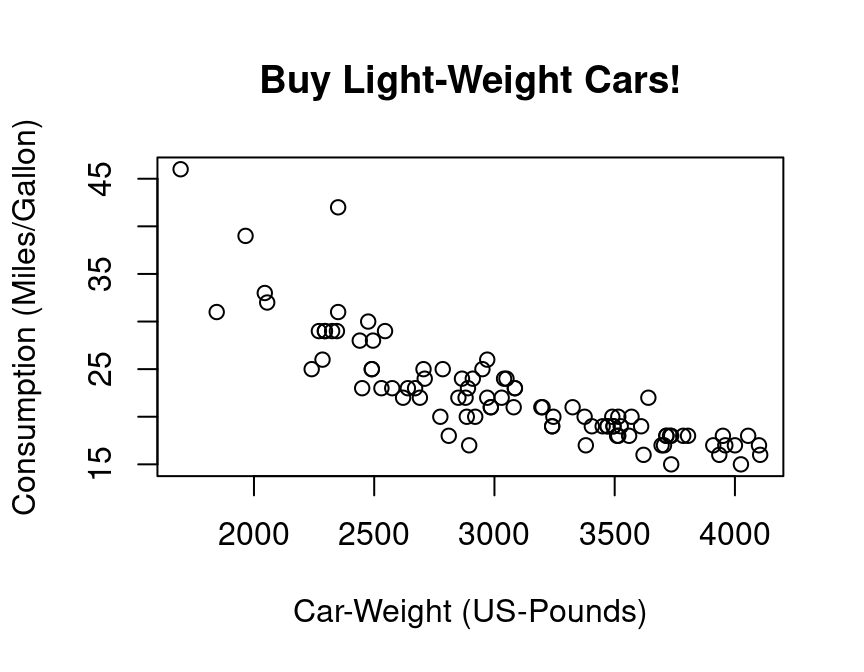
\includegraphics{01-Introduction-to-R_files/figure-latex/fig-margin-1.pdf}

\hfill\break

As a first step, we might assume a simple kind of linear relationship between the variables \texttt{gasolin.consumption} and \texttt{car.weight}. Let us assume that the data was generated by the following simple regression model:
\[
y_i=\alpha+\beta_1 x_i+\varepsilon_i,\quad i=1,\dots,n
\]
where \(y_i\) denotes the gasoline-consumption, \(x_i\) the weight of car \(i\), and \(\varepsilon_i\) is a mean zero constant variance noise term. (This is clearly a non-sense model!)

The command \texttt{lm()} computes the estimates of this linear regression model. The command (in fact it's a \emph{method}) \texttt{summary()} computes further quantities of general interest from the \emph{object} that was returned from the \texttt{lm()} function.

\begin{Shaded}
\begin{Highlighting}[]
\NormalTok{lm.result   }\OtherTok{\textless{}{-}} \FunctionTok{lm}\NormalTok{(gasolin.consumption}\SpecialCharTok{\textasciitilde{}}\NormalTok{car.weight)}
\NormalTok{lm.summary  }\OtherTok{\textless{}{-}} \FunctionTok{summary}\NormalTok{(lm.result)}
\NormalTok{lm.summary}
\end{Highlighting}
\end{Shaded}

\begin{verbatim}
## 
## Call:
## lm(formula = gasolin.consumption ~ car.weight)
## 
## Residuals:
##     Min      1Q  Median      3Q     Max 
## -6.7946 -1.9711  0.0249  1.1855 13.8278 
## 
## Coefficients:
##              Estimate Std. Error t value Pr(>|t|)    
## (Intercept) 47.048353   1.679912   28.01   <2e-16 ***
## car.weight  -0.008032   0.000537  -14.96   <2e-16 ***
## ---
## Signif. codes:  0 '***' 0.001 '**' 0.01 '*' 0.05 '.' 0.1 ' ' 1
## 
## Residual standard error: 3.038 on 91 degrees of freedom
## Multiple R-squared:  0.7109, Adjusted R-squared:  0.7077 
## F-statistic: 223.8 on 1 and 91 DF,  p-value: < 2.2e-16
\end{verbatim}

\hfill\break

Of course, we want to have a possibility to access all the quantities computed so far, e.g., in order to plot the results. This can be done as following:

\begin{Shaded}
\begin{Highlighting}[]
\DocumentationTok{\#\# Accessing the computed quantities}
\FunctionTok{names}\NormalTok{(lm.summary) }\DocumentationTok{\#\# Alternatively: str(lm.summary)}
\end{Highlighting}
\end{Shaded}

\begin{verbatim}
##  [1] "call"          "terms"         "residuals"     "coefficients" 
##  [5] "aliased"       "sigma"         "df"            "r.squared"    
##  [9] "adj.r.squared" "fstatistic"    "cov.unscaled"
\end{verbatim}

\begin{Shaded}
\begin{Highlighting}[]
\NormalTok{alpha }\OtherTok{\textless{}{-}}\NormalTok{ lm.summary}\SpecialCharTok{$}\NormalTok{coefficients[}\DecValTok{1}\NormalTok{]}
\NormalTok{beta  }\OtherTok{\textless{}{-}}\NormalTok{ lm.summary}\SpecialCharTok{$}\NormalTok{coefficients[}\DecValTok{2}\NormalTok{]}

\DocumentationTok{\#\# Plot all:}
\FunctionTok{plot}\NormalTok{(}\AttributeTok{y=}\NormalTok{gasolin.consumption, }\AttributeTok{x=}\NormalTok{car.weight, }
     \AttributeTok{xlab=}\StringTok{"Car{-}Weight (US{-}Pounds)"}\NormalTok{, }
     \AttributeTok{ylab=}\StringTok{"Consumption (Miles/Gallon)"}\NormalTok{, }
     \AttributeTok{main=}\StringTok{"Buy light{-}weight Cars!"}\NormalTok{)}
\FunctionTok{abline}\NormalTok{(}\AttributeTok{a=}\NormalTok{alpha, }
       \AttributeTok{b=}\NormalTok{beta, }\AttributeTok{col=}\StringTok{"red"}\NormalTok{)}
\end{Highlighting}
\end{Shaded}

\begin{center}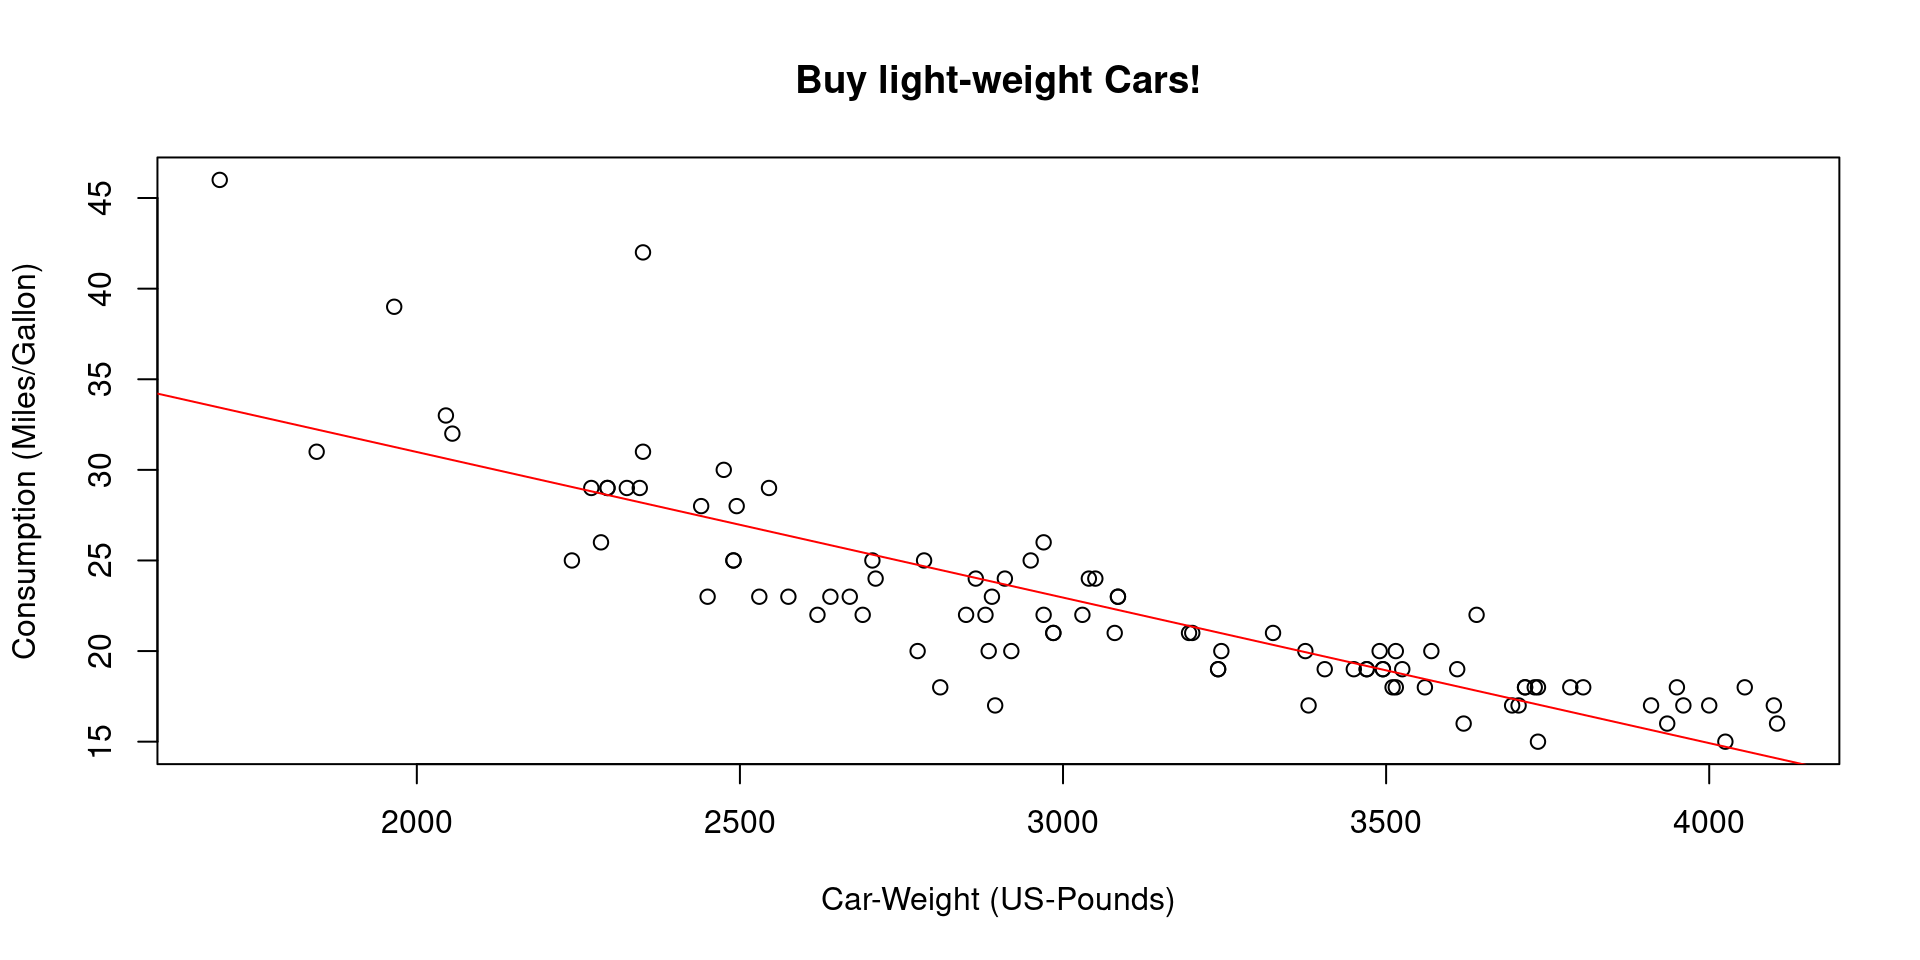
\includegraphics[width=\textwidth]{01-Introduction-to-R_files/figure-latex/unnamed-chunk-23-1} \end{center}

\hfill\break

\hypertarget{programming-in-r}{%
\section{Programming in R}\label{programming-in-r}}

Let's write, i.e., program our own R-function for estimating linear regression models. In order to be able to validate our function, we start with \textbf{simulating data} for which we then \emph{know} all true parameters. Simulating data is like being the ``Data-God'': For instance, we generate realizations of the error term \(\varepsilon_i\), i.e., something which we \emph{never} observe in real data.

\hfill\break

Let us consider the following multiple regression model:

\[y_i=\beta_1 +\beta_2 x_{2i}+\beta_3 x_{3i}+\varepsilon_{i},\quad i=1,\dots,n,\]
where \(\varepsilon_{i}\) is a heteroscedastic error term
\[\varepsilon_{i}\sim N(0,\sigma_i^2),\quad \sigma_i=x_{3i},\]

and where for all \(i=1,\dots,n=50\):

\begin{itemize}
\tightlist
\item
  \(x_{2i}\sim N(10,1.5^2)\)
\item
  \(x_{3i}\) comes from a t-distribution with 5 degrees of freedom and non-centrality parameter 2
\end{itemize}

\begin{Shaded}
\begin{Highlighting}[]
\FunctionTok{set.seed}\NormalTok{(}\DecValTok{109}\NormalTok{) }\CommentTok{\# Sets the "seed" of the random number generators:}
\NormalTok{n   }\OtherTok{\textless{}{-}} \DecValTok{50}     \CommentTok{\# Number of observations}

\DocumentationTok{\#\# Generate two explanatory variables plus an intercept{-}variable:}
\NormalTok{X}\FloatTok{.1} \OtherTok{\textless{}{-}} \FunctionTok{rep}\NormalTok{(}\DecValTok{1}\NormalTok{, n)                 }\CommentTok{\# Intercept}
\NormalTok{X}\FloatTok{.2} \OtherTok{\textless{}{-}} \FunctionTok{rnorm}\NormalTok{(n, }\AttributeTok{mean=}\DecValTok{10}\NormalTok{, }\AttributeTok{sd=}\FloatTok{1.5}\NormalTok{) }\CommentTok{\# Draw realizations form a normal distr.}
\NormalTok{X}\FloatTok{.3} \OtherTok{\textless{}{-}} \FunctionTok{rt}\NormalTok{(n, }\AttributeTok{df=}\DecValTok{5}\NormalTok{, }\AttributeTok{ncp=}\DecValTok{2}\NormalTok{)        }\CommentTok{\# Draw realizations form a t{-}distr.}
\NormalTok{X   }\OtherTok{\textless{}{-}} \FunctionTok{cbind}\NormalTok{(X}\FloatTok{.1}\NormalTok{, X}\FloatTok{.2}\NormalTok{, X}\FloatTok{.3}\NormalTok{)      }\CommentTok{\# Save as a Nx3{-}dimensional data matrix.}
\end{Highlighting}
\end{Shaded}

OK, we have regressors, i.e., data that we also have in real data sets.

Now we define the elements of the \(\beta\)-vector. Be aware of the difference: In real data sets we do not know the true \(\beta\)-vector, but try to estimate it. However, when simulating data, we determine (as ``Data-Gods'') the true \(\beta\)-vector and can compare our estimate \(\hat{\beta}\) with the true \(\beta\):

\begin{Shaded}
\begin{Highlighting}[]
\DocumentationTok{\#\# Define the slope{-}coefficients}
\NormalTok{beta.vec  }\OtherTok{\textless{}{-}} \FunctionTok{c}\NormalTok{(}\DecValTok{1}\NormalTok{,}\SpecialCharTok{{-}}\DecValTok{5}\NormalTok{,}\DecValTok{5}\NormalTok{)}
\end{Highlighting}
\end{Shaded}

\hfill\break
We still need to simulate realizations of the dependent variable \(y_i\). Remember that \(y_i=\beta_1 x_{1i}+\beta_1 x_{2i}+\beta_3 x_{3i}+\varepsilon_{i}\). That is, we only need realizations from the error terms \(\varepsilon_i\) in order to compute the realizations from \(y_i\). This is how you can simulate realizations from the heteroscedastic error terms \(\varepsilon_i\):

\begin{Shaded}
\begin{Highlighting}[]
\DocumentationTok{\#\# Generate realizations from the heteroscadastic error term}
\NormalTok{eps       }\OtherTok{\textless{}{-}}\NormalTok{ (X}\FloatTok{.3}\NormalTok{)}\SpecialCharTok{*}\FunctionTok{rnorm}\NormalTok{(n, }\AttributeTok{mean=}\DecValTok{0}\NormalTok{, }\AttributeTok{sd=}\DecValTok{1}\NormalTok{)}
\end{Highlighting}
\end{Shaded}

Take a look at the heteroscedasticity in the error term:

\begin{Shaded}
\begin{Highlighting}[]
\FunctionTok{plot}\NormalTok{(}\AttributeTok{y=}\NormalTok{eps, }\AttributeTok{x=}\NormalTok{X}\FloatTok{.3}\NormalTok{, }
     \AttributeTok{main=}\StringTok{"Realizations of the }\SpecialCharTok{\textbackslash{}n}\StringTok{Heteroscedastic Error Term"}\NormalTok{)}
\end{Highlighting}
\end{Shaded}

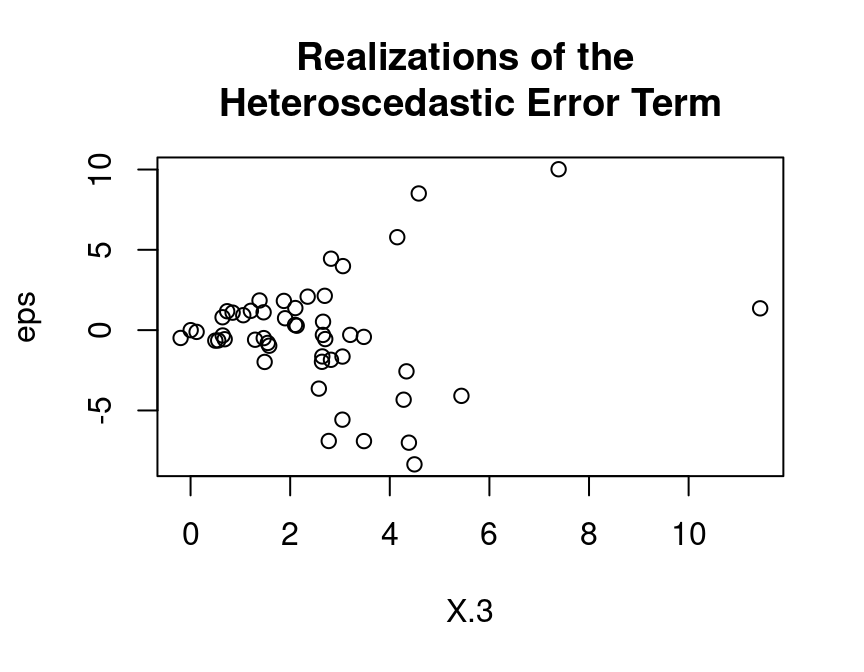
\includegraphics{01-Introduction-to-R_files/figure-latex/unnamed-chunk-27-1.pdf}

With the (pseudo-random) realizations from \(\varepsilon_i\), we can finally generate realizations from the dependent variable \(y_i\):

\begin{Shaded}
\begin{Highlighting}[]
\DocumentationTok{\#\# Dependent variable:}
\NormalTok{y   }\OtherTok{\textless{}{-}}\NormalTok{ X }\SpecialCharTok{\%*\%}\NormalTok{ beta.vec }\SpecialCharTok{+}\NormalTok{ eps}
\end{Highlighting}
\end{Shaded}

Let's take a look at the data:

\begin{Shaded}
\begin{Highlighting}[]
\NormalTok{mydata    }\OtherTok{\textless{}{-}} \FunctionTok{data.frame}\NormalTok{(}\StringTok{"Y"}\OtherTok{=}\NormalTok{y, }\StringTok{"X.1"}\OtherTok{=}\NormalTok{X}\FloatTok{.1}\NormalTok{, }\StringTok{"X.2"}\OtherTok{=}\NormalTok{X}\FloatTok{.2}\NormalTok{, }\StringTok{"X.3"}\OtherTok{=}\NormalTok{X}\FloatTok{.3}\NormalTok{)}
\FunctionTok{pairs}\NormalTok{(mydata[,}\SpecialCharTok{{-}}\DecValTok{2}\NormalTok{]) }\CommentTok{\# The \textquotesingle{}{-}2\textquotesingle{} removes the intercept variable "X.1"}
\end{Highlighting}
\end{Shaded}

\begin{center}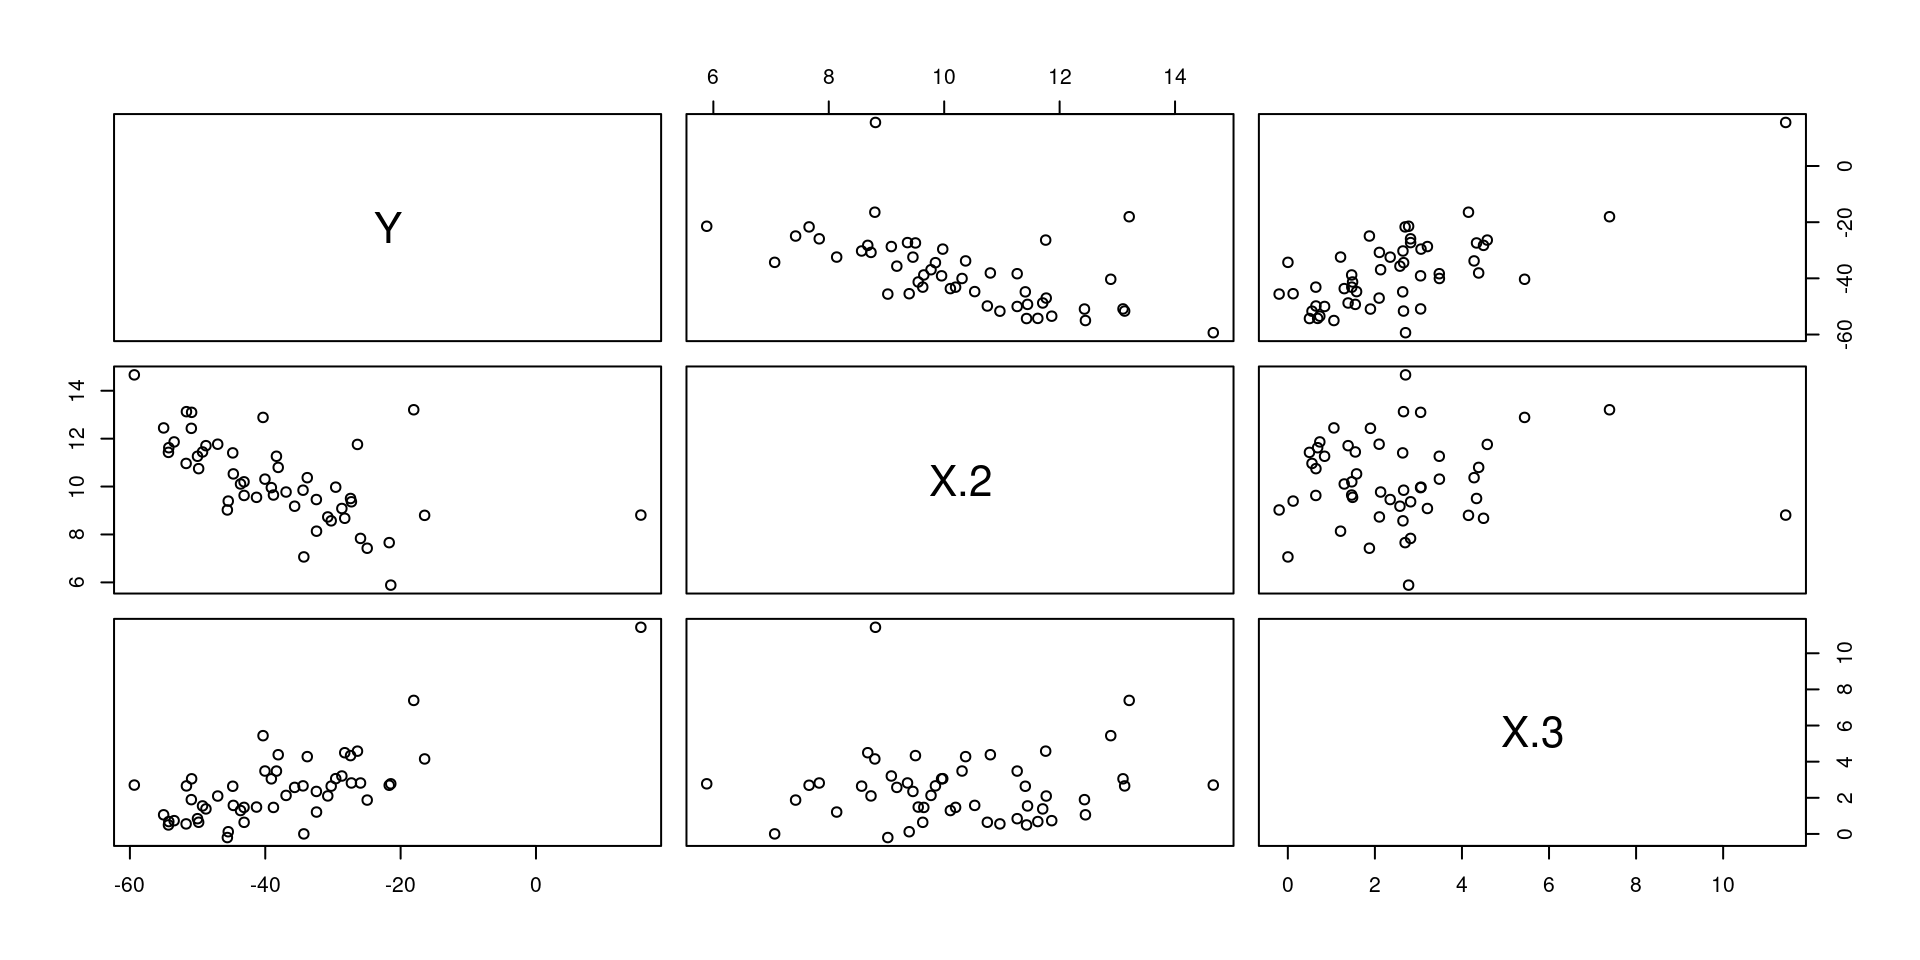
\includegraphics[width=\textwidth]{01-Introduction-to-R_files/figure-latex/unnamed-chunk-29-1} \end{center}

\hfill\break

Once we have data, we can compute the OLS estimate of the true \(\beta\) vector. Remember the formula:
\[\hat{\beta}=(X^\top X)^{-1}X^\top y\]
In R-Code this is: \((X^\top X)^{-1}=\)\texttt{solve(t(X)\ \%*\%\ X)}, i.e.:

\begin{Shaded}
\begin{Highlighting}[]
\DocumentationTok{\#\# Computation of the beta{-}Vector:}
\NormalTok{beta.hat }\OtherTok{\textless{}{-}} \FunctionTok{solve}\NormalTok{(}\FunctionTok{t}\NormalTok{(X) }\SpecialCharTok{\%*\%}\NormalTok{ X) }\SpecialCharTok{\%*\%} \FunctionTok{t}\NormalTok{(X) }\SpecialCharTok{\%*\%}\NormalTok{ y}
\NormalTok{beta.hat}
\end{Highlighting}
\end{Shaded}

\begin{verbatim}
##          [,1]
## X.1 -2.735042
## X.2 -4.685719
## X.3  5.091811
\end{verbatim}

\hfill\break

Well done. Using the above lines of code we can easily program our own \texttt{myOLSFun()} function!

\begin{Shaded}
\begin{Highlighting}[]
\NormalTok{myOLSFun }\OtherTok{\textless{}{-}} \ControlFlowTok{function}\NormalTok{(y, x, }\AttributeTok{add.intercept=}\ConstantTok{FALSE}\NormalTok{)\{}
  
  \DocumentationTok{\#\# Number of Observations:}
\NormalTok{  n         }\OtherTok{\textless{}{-}} \FunctionTok{length}\NormalTok{(y)}
  
  \DocumentationTok{\#\# Add an intercept to x:}
  \ControlFlowTok{if}\NormalTok{(add.intercept)\{}
\NormalTok{    Intercept }\OtherTok{\textless{}{-}} \FunctionTok{rep}\NormalTok{(}\DecValTok{1}\NormalTok{, n)}
\NormalTok{    x         }\OtherTok{\textless{}{-}} \FunctionTok{cbind}\NormalTok{(Intercept, x)}
\NormalTok{  \}}
  
  \DocumentationTok{\#\# Estimation of the slope{-}parameters:}
\NormalTok{  beta.hat.vec }\OtherTok{\textless{}{-}} \FunctionTok{solve}\NormalTok{(}\FunctionTok{t}\NormalTok{(x) }\SpecialCharTok{\%*\%}\NormalTok{ x) }\SpecialCharTok{\%*\%} \FunctionTok{t}\NormalTok{(x) }\SpecialCharTok{\%*\%}\NormalTok{ y}
  
  \DocumentationTok{\#\# Return the result:}
  \FunctionTok{return}\NormalTok{(beta.hat.vec)}
\NormalTok{\}}

\DocumentationTok{\#\# Run the function:}
\FunctionTok{myOLSFun}\NormalTok{(}\AttributeTok{y=}\NormalTok{y, }\AttributeTok{x=}\NormalTok{X)}
\end{Highlighting}
\end{Shaded}

\begin{verbatim}
##          [,1]
## X.1 -2.735042
## X.2 -4.685719
## X.3  5.091811
\end{verbatim}

\hfill\break

Can you extend the function for the computation of the covariance matrix of the slope-estimates, several measures of fits (R\(^2\), adj.-R\(^2\), etc.), t-tests, \ldots?

\hypertarget{r-packages}{%
\section{R-packages}\label{r-packages}}

One of the best features in R are its contributed packages. The list of all packages on CRAN is impressive! Take a look at it \href{https://cran.r-project.org/web/packages/available_packages_by_name.html}{HERE}

For instance, nice plots can be produced using the R-package is \texttt{ggplot2}. You can find an intro do this package \href{http://ggplot2.tidyverse.org/}{HERE}.

\begin{Shaded}
\begin{Highlighting}[]
\CommentTok{\# install.packages("ggplot2")}
\FunctionTok{library}\NormalTok{(}\StringTok{"ggplot2"}\NormalTok{)}

\FunctionTok{qplot}\NormalTok{(Sepal.Length, Petal.Length, }\AttributeTok{data =}\NormalTok{ iris, }\AttributeTok{color =}\NormalTok{ Species)}
\end{Highlighting}
\end{Shaded}

\begin{center}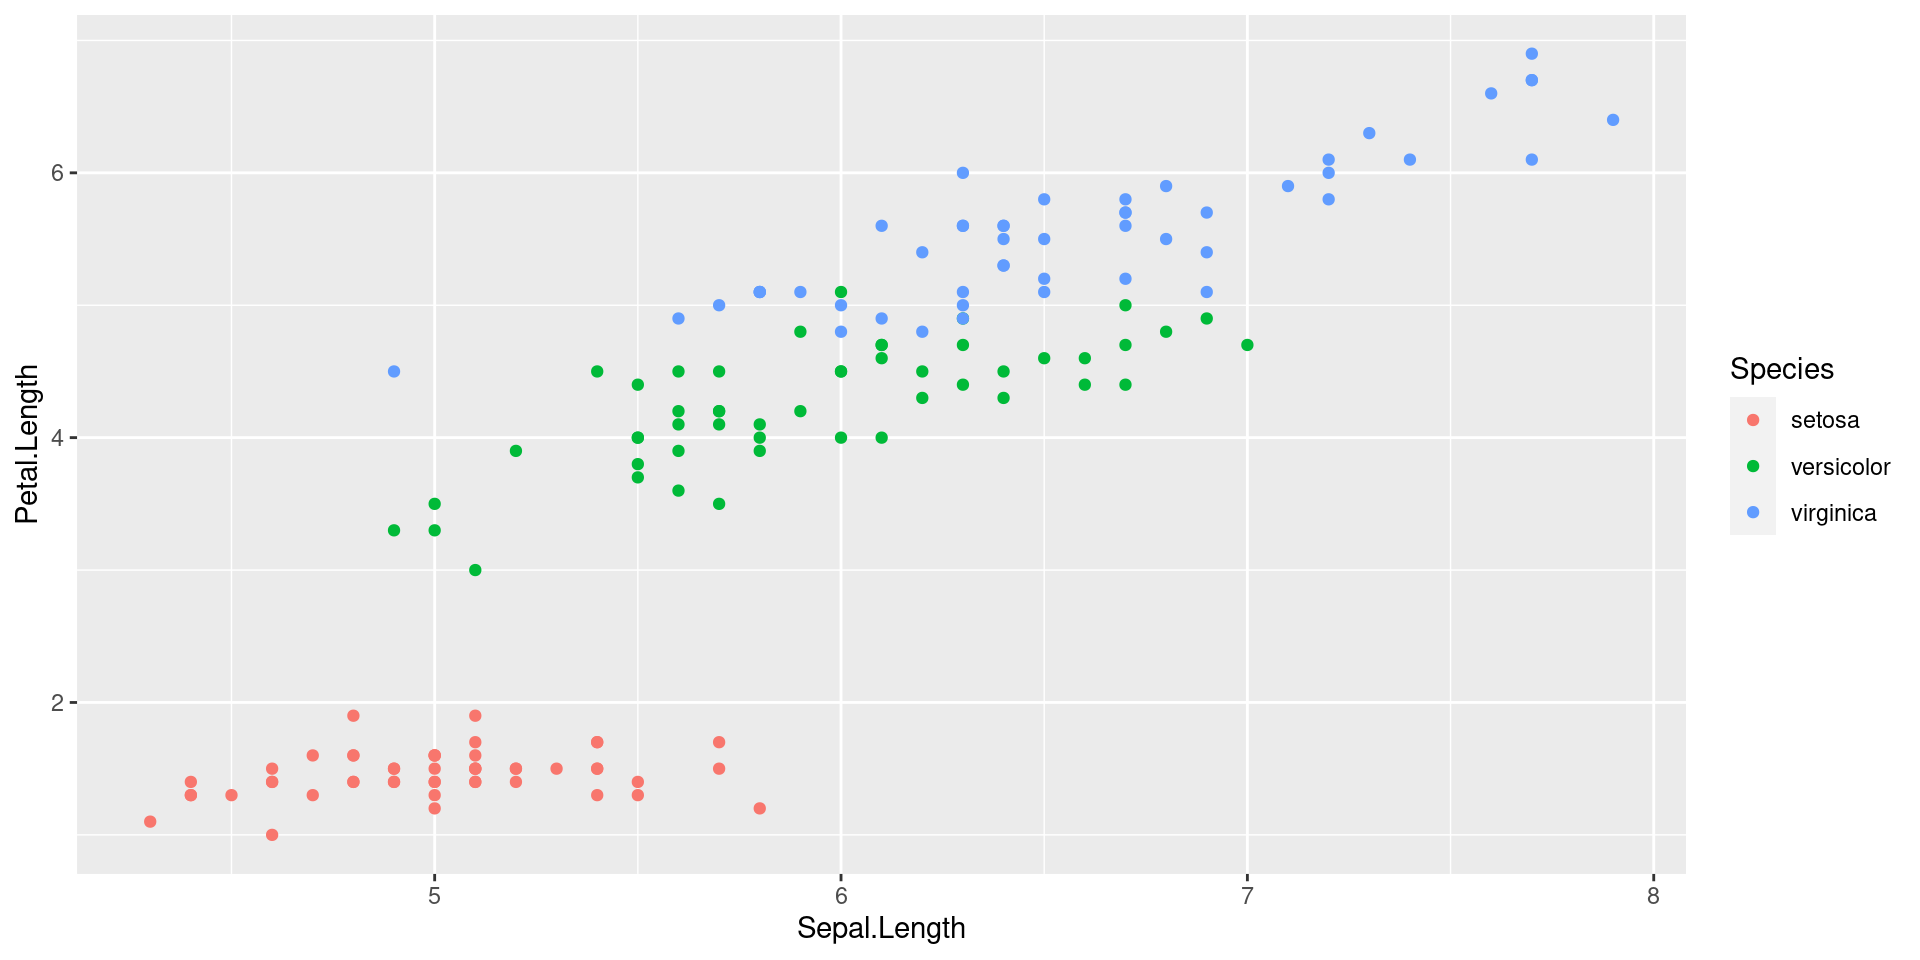
\includegraphics[width=\textwidth]{01-Introduction-to-R_files/figure-latex/unnamed-chunk-32-1} \end{center}

\hfill\break

Of course, \texttt{ggplot2} concerns ``only'' plotting, but you'll find R-packages for almost any statistical method out there.

\hypertarget{tidyverse}{%
\section{Tidyverse}\label{tidyverse}}

The \texttt{tidyverse} package is a collection of packages that lets you import,
manipulate, explore, visualize and model data in a harmonized and consistent way which
helps you to be more productive.

Installing the \texttt{tidyverse} package:

\begin{Shaded}
\begin{Highlighting}[]
\FunctionTok{install.packages}\NormalTok{(}\StringTok{"tidyverse"}\NormalTok{)}
\end{Highlighting}
\end{Shaded}

To use the \texttt{tidyverse} package load it using the \texttt{library()} function:

\begin{Shaded}
\begin{Highlighting}[]
\FunctionTok{library}\NormalTok{(tidyverse)}
\end{Highlighting}
\end{Shaded}

\begin{verbatim}
## -- Attaching packages --------------------------------------- tidyverse 1.3.0 --
\end{verbatim}

\begin{verbatim}
## v tibble  3.1.5     v dplyr   1.0.4
## v tidyr   1.1.2     v stringr 1.4.0
## v purrr   0.3.4     v forcats 0.5.1
\end{verbatim}

\begin{verbatim}
## -- Conflicts ------------------------------------------ tidyverse_conflicts() --
## x dplyr::filter() masks stats::filter()
## x dplyr::lag()    masks stats::lag()
\end{verbatim}

\textbf{Chick Weight Data}

R comes with many datasets installed. We will use the \texttt{ChickWeight} dataset
to learn about the tidyverse. The help system gives a basic summary of the experiment from
which the data was collect:

\begin{quote}
\emph{``The body weights of the chicks were measured at birth and every second day thereafter
until day 20. They were also measured on day 21. There were four groups of chicks on
different protein diets.''}
\end{quote}

You can get more information, including references by typing:

\begin{Shaded}
\begin{Highlighting}[]
\FunctionTok{help}\NormalTok{(}\StringTok{"ChickWeight"}\NormalTok{)}
\end{Highlighting}
\end{Shaded}

\textbf{The Data: }
There are 578 observations (rows) and 4 variables:

\begin{itemize}
\tightlist
\item
  \texttt{Chick} -- unique ID for each chick.
\item
  \texttt{Diet} -- one of four protein diets.
\item
  \texttt{Time} -- number of days since birth.
\item
  \texttt{weight} -- body weight of chick in grams.
\end{itemize}

Note: \texttt{weight} has a lower case \texttt{w} (recall R is case sensitive).

Store the data locally:

\begin{Shaded}
\begin{Highlighting}[]
\NormalTok{ChickWeight }\SpecialCharTok{\%\textgreater{}\%}
  \FunctionTok{select}\NormalTok{(Chick, Diet, Time, weight) }\SpecialCharTok{\%\textgreater{}\%} 
  \FunctionTok{arrange}\NormalTok{(Chick, Diet, Time) }\SpecialCharTok{\%\textgreater{}\%} 
  \FunctionTok{write\_csv}\NormalTok{(}\StringTok{"ChickWeight.csv"}\NormalTok{)}
\end{Highlighting}
\end{Shaded}

First we will import the data from a file called \texttt{ChickWeight.csv} using the \texttt{read\_csv()}
function from the \texttt{readr} package (part of the \texttt{tidyverse}). The first thing to do,
outside of R, is to open the file \texttt{ChickWeight.csv} to check what it contains and that
it makes sense. Now we can import the data as follows:

\begin{Shaded}
\begin{Highlighting}[]
\NormalTok{CW }\OtherTok{\textless{}{-}} \FunctionTok{read\_csv}\NormalTok{(}\StringTok{"ChickWeight.csv"}\NormalTok{)}
\end{Highlighting}
\end{Shaded}

\begin{verbatim}
## 
## -- Column specification --------------------------------------------------------
## cols(
##   Chick = col_double(),
##   Diet = col_double(),
##   Time = col_double(),
##   weight = col_double()
## )
\end{verbatim}

If all goes well then the data is now stored in an R object called \texttt{CW}. If you get the
following error message then you need to change the working directory to where the data is
stored.

\begin{verbatim}
Error: 'ChickWeight.csv' does not exist in current
working directory ...
\end{verbatim}

\textbf{Changing the working directory:}
In RStudio you can use the menu bar (``Session - Set Working Directory - Choose Directory\ldots{}''). Alternatively, you can use the function \texttt{setwd()}.

\hfill\break

\textbf{Looking at the Dataset:}
To look at the data type just type the object (dataset) name:

\begin{Shaded}
\begin{Highlighting}[]
\NormalTok{CW}
\end{Highlighting}
\end{Shaded}

\begin{verbatim}
## # A tibble: 578 x 4
##    Chick  Diet  Time weight
##    <dbl> <dbl> <dbl>  <dbl>
##  1    18     1     0     39
##  2    18     1     2     35
##  3    16     1     0     41
##  4    16     1     2     45
##  5    16     1     4     49
##  6    16     1     6     51
##  7    16     1     8     57
##  8    16     1    10     51
##  9    16     1    12     54
## 10    15     1     0     41
## # ... with 568 more rows
\end{verbatim}

If there are too many variables then not all them may be printed. To overcome this issue
we can use the \texttt{glimpse()} function which makes it possible to see every column in your
dataset (called a ``data frame'' in R speak).

\begin{Shaded}
\begin{Highlighting}[]
\FunctionTok{glimpse}\NormalTok{(CW)}
\end{Highlighting}
\end{Shaded}

\begin{verbatim}
## Rows: 578
## Columns: 4
## $ Chick  <dbl> 18, 18, 16, 16, 16, 16, 16, 16, 16, 15, 15, 15, 15, 15, 15, 15,~
## $ Diet   <dbl> 1, 1, 1, 1, 1, 1, 1, 1, 1, 1, 1, 1, 1, 1, 1, 1, 1, 1, 1, 1, 1, ~
## $ Time   <dbl> 0, 2, 0, 2, 4, 6, 8, 10, 12, 0, 2, 4, 6, 8, 10, 12, 14, 0, 2, 4~
## $ weight <dbl> 39, 35, 41, 45, 49, 51, 57, 51, 54, 41, 49, 56, 64, 68, 68, 67,~
\end{verbatim}

The function \texttt{View()} allows for a spread-sheet type of view on the data:

\begin{Shaded}
\begin{Highlighting}[]
\FunctionTok{View}\NormalTok{(CW)}
\end{Highlighting}
\end{Shaded}

\hypertarget{tidyverse-plotting-basics}{%
\subsection{Tidyverse: Plotting Basics}\label{tidyverse-plotting-basics}}

To \textbf{visualise} the chick weight data, we will use the \texttt{ggplot2} package (part of the
\texttt{tidyverse}). Our interest is in seeing how the \emph{weight changes over time for the chicks by
diet}. For the moment don't worry too much about the details just try to build your own
understanding and logic. To learn more try different things even if you get an error
messages.

Let's plot the weight data (vertical axis) over time (horizontal axis).

\begin{Shaded}
\begin{Highlighting}[]
\CommentTok{\# An empty plot (the plot on the left)}
\FunctionTok{ggplot}\NormalTok{(CW, }\FunctionTok{aes}\NormalTok{(Time, weight))  }
\CommentTok{\# With data (the plot on the right)}
\FunctionTok{ggplot}\NormalTok{(CW, }\FunctionTok{aes}\NormalTok{(Time, weight)) }\SpecialCharTok{+} \FunctionTok{geom\_point}\NormalTok{() }
\end{Highlighting}
\end{Shaded}

\begin{center}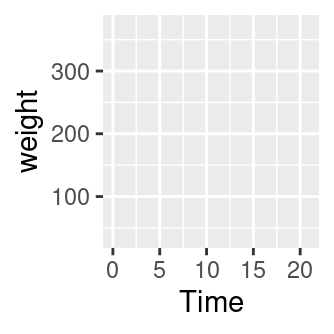
\includegraphics{01-Introduction-to-R_files/figure-latex/emptyPlot-1} 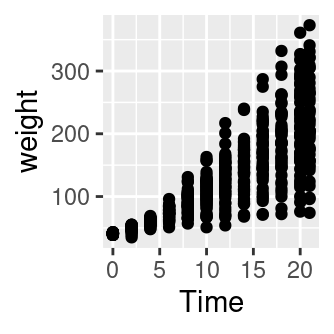
\includegraphics{01-Introduction-to-R_files/figure-latex/emptyPlot-2} \end{center}

Add color for \texttt{Diet}. The graph above does not differentiate between the diets. Let's use a different color for
each diet.

\begin{Shaded}
\begin{Highlighting}[]
\CommentTok{\# Adding colour for diet}
\FunctionTok{ggplot}\NormalTok{(CW,}\FunctionTok{aes}\NormalTok{(Time,weight,}\AttributeTok{colour=}\FunctionTok{factor}\NormalTok{(Diet))) }\SpecialCharTok{+}
  \FunctionTok{geom\_point}\NormalTok{() }
\end{Highlighting}
\end{Shaded}

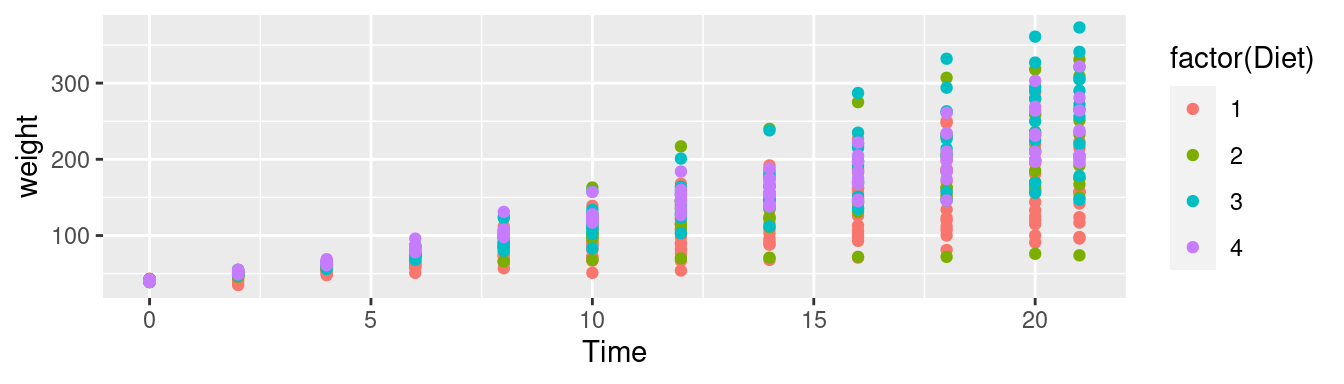
\includegraphics{01-Introduction-to-R_files/figure-latex/addColourPlot-1.pdf}

It is difficult to conclude anything from this graph as the points are printed on top of
one another (with diet 1 underneath and diet 4 at the top).

\textbf{Factor Variables:}
Before we continue, we have to make an important change to the \texttt{CW} dataset by making
\texttt{Diet} and \texttt{Time} \emph{factor variables}. This means that R will treat them as categorical
variables (see the \texttt{\textless{}fct\textgreater{}} variables below) instead of continuous variables. It will
simplify our coding. The next section will explain the \texttt{mutate()} function.

\begin{Shaded}
\begin{Highlighting}[]
\NormalTok{CW }\OtherTok{\textless{}{-}} \FunctionTok{mutate}\NormalTok{(CW, }\AttributeTok{Diet =} \FunctionTok{factor}\NormalTok{(Diet))}
\NormalTok{CW }\OtherTok{\textless{}{-}} \FunctionTok{mutate}\NormalTok{(CW, }\AttributeTok{Time =} \FunctionTok{factor}\NormalTok{(Time))}
\FunctionTok{glimpse}\NormalTok{(CW)}
\end{Highlighting}
\end{Shaded}

\begin{verbatim}
## Rows: 578
## Columns: 4
## $ Chick  <dbl> 18, 18, 16, 16, 16, 16, 16, 16, 16, 15, 15, 15, 15, 15, 15, 15,~
## $ Diet   <fct> 1, 1, 1, 1, 1, 1, 1, 1, 1, 1, 1, 1, 1, 1, 1, 1, 1, 1, 1, 1, 1, ~
## $ Time   <fct> 0, 2, 0, 2, 4, 6, 8, 10, 12, 0, 2, 4, 6, 8, 10, 12, 14, 0, 2, 4~
## $ weight <dbl> 39, 35, 41, 45, 49, 51, 57, 51, 54, 41, 49, 56, 64, 68, 68, 67,~
\end{verbatim}

The \texttt{facet\_wrap()} function: To plot each diet separately in a grid using \texttt{facet\_wrap()}:

\begin{Shaded}
\begin{Highlighting}[]
\CommentTok{\# Adding jitter to the points}
\FunctionTok{ggplot}\NormalTok{(CW, }\FunctionTok{aes}\NormalTok{(Time, weight, }\AttributeTok{colour=}\NormalTok{Diet)) }\SpecialCharTok{+}
  \FunctionTok{geom\_point}\NormalTok{() }\SpecialCharTok{+}
  \FunctionTok{facet\_wrap}\NormalTok{(}\SpecialCharTok{\textasciitilde{}}\NormalTok{Diet) }\SpecialCharTok{+}
  \FunctionTok{theme}\NormalTok{(}\AttributeTok{legend.position =} \StringTok{"bottom"}\NormalTok{)}
\end{Highlighting}
\end{Shaded}

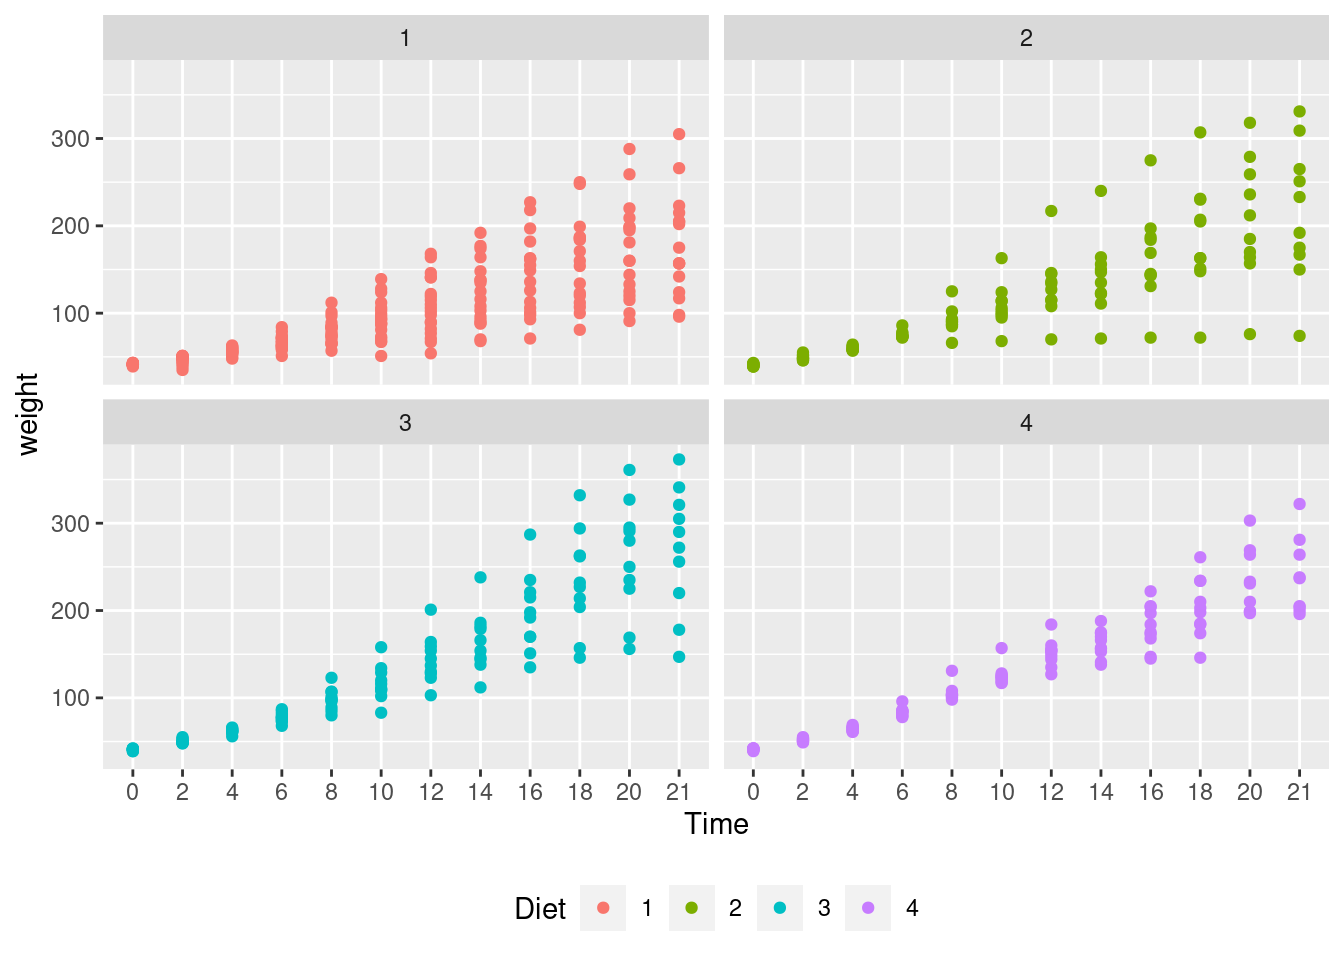
\includegraphics{01-Introduction-to-R_files/figure-latex/ScatterPlot-1.pdf}

\textbf{Interpretation:} Diet 4 has the least variability but we can't really say anything about the mean effect
of each diet although diet 3 seems to have the highest.

Next we will plot the \textbf{mean changes} over time for each diet using the \texttt{stat\_summary()} function:

\begin{Shaded}
\begin{Highlighting}[]
\FunctionTok{ggplot}\NormalTok{(CW, }\FunctionTok{aes}\NormalTok{(Time, weight, }
               \AttributeTok{group=}\NormalTok{Diet, }\AttributeTok{colour=}\NormalTok{Diet)) }\SpecialCharTok{+}
  \FunctionTok{stat\_summary}\NormalTok{(}\AttributeTok{fun.y=}\StringTok{"mean"}\NormalTok{, }\AttributeTok{geom=}\StringTok{"line"}\NormalTok{) }
\end{Highlighting}
\end{Shaded}

\begin{verbatim}
## Warning: `fun.y` is deprecated. Use `fun` instead.
\end{verbatim}

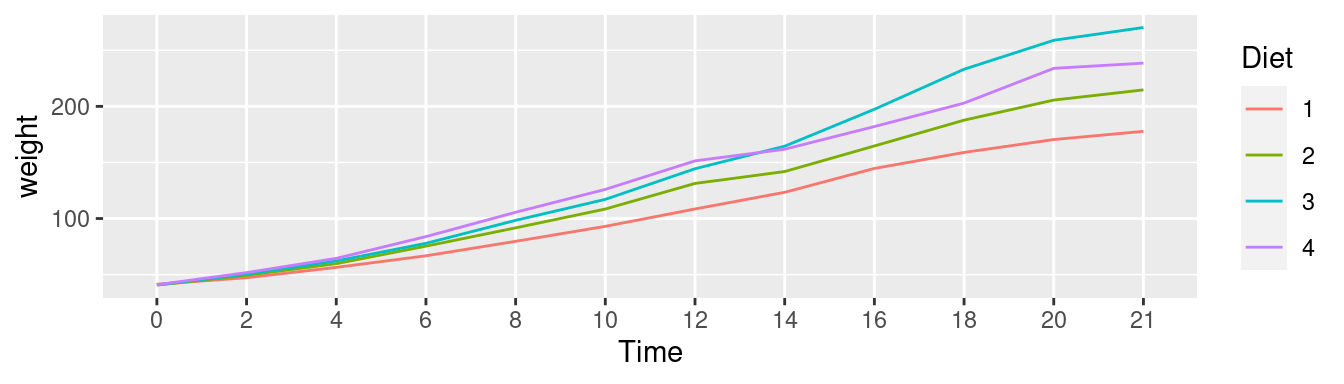
\includegraphics{01-Introduction-to-R_files/figure-latex/meanlinesPlot-1.pdf}

\textbf{Interpretation:}
We can see that diet 3 has the highest mean weight gains by the end of the experiment. However,
we don't have any information about the variation (uncertainty) in the data.

To see variation between the different diets we use \texttt{geom\_boxplot} to plot a box-whisker plot.
A note of caution is that the number of chicks per diet is relatively low to produce this plot.

\begin{Shaded}
\begin{Highlighting}[]
\FunctionTok{ggplot}\NormalTok{(CW, }\FunctionTok{aes}\NormalTok{(Time, weight, }\AttributeTok{colour=}\NormalTok{Diet)) }\SpecialCharTok{+}
  \FunctionTok{facet\_wrap}\NormalTok{(}\SpecialCharTok{\textasciitilde{}}\NormalTok{Diet) }\SpecialCharTok{+}
  \FunctionTok{geom\_boxplot}\NormalTok{() }\SpecialCharTok{+}
  \FunctionTok{theme}\NormalTok{(}\AttributeTok{legend.position =} \StringTok{"none"}\NormalTok{) }\SpecialCharTok{+}
  \FunctionTok{ggtitle}\NormalTok{(}\StringTok{"Chick Weight over Time by Diet"}\NormalTok{)}
\end{Highlighting}
\end{Shaded}

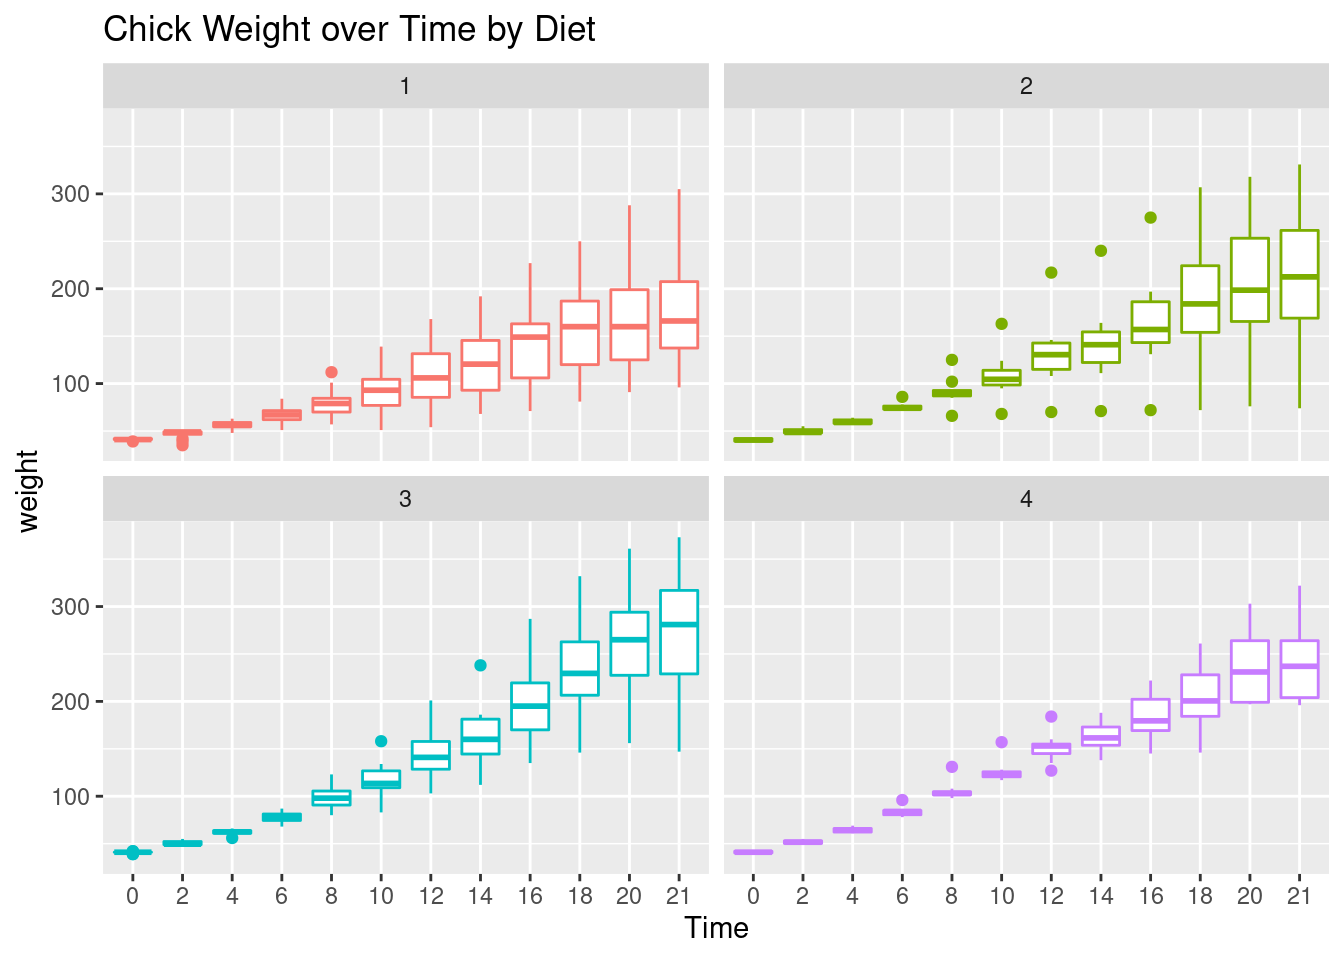
\includegraphics{01-Introduction-to-R_files/figure-latex/boxPlot-1.pdf}

\textbf{Interpretation:}
Diet 3 seems to have the highest ``average'' weight gain but it has more variation
than diet 4 which is consistent with our findings so far.

Let's finish with a plot that you might include in a publication.

\begin{Shaded}
\begin{Highlighting}[]
\FunctionTok{ggplot}\NormalTok{(CW, }\FunctionTok{aes}\NormalTok{(Time, weight, }\AttributeTok{group=}\NormalTok{Diet, }
                             \AttributeTok{colour=}\NormalTok{Diet)) }\SpecialCharTok{+}
  \FunctionTok{facet\_wrap}\NormalTok{(}\SpecialCharTok{\textasciitilde{}}\NormalTok{Diet) }\SpecialCharTok{+}
  \FunctionTok{geom\_point}\NormalTok{() }\SpecialCharTok{+}
  \CommentTok{\# geom\_jitter() +}
  \FunctionTok{stat\_summary}\NormalTok{(}\AttributeTok{fun.y=}\StringTok{"mean"}\NormalTok{, }\AttributeTok{geom=}\StringTok{"line"}\NormalTok{,}
               \AttributeTok{colour=}\StringTok{"black"}\NormalTok{) }\SpecialCharTok{+}
  \FunctionTok{theme}\NormalTok{(}\AttributeTok{legend.position =} \StringTok{"none"}\NormalTok{) }\SpecialCharTok{+}
  \FunctionTok{ggtitle}\NormalTok{(}\StringTok{"Chick Weight over Time by Diet"}\NormalTok{) }\SpecialCharTok{+} 
  \FunctionTok{xlab}\NormalTok{(}\StringTok{"Time (days)"}\NormalTok{) }\SpecialCharTok{+}
  \FunctionTok{ylab}\NormalTok{(}\StringTok{"Weight (grams)"}\NormalTok{)}
\end{Highlighting}
\end{Shaded}

\begin{verbatim}
## Warning: `fun.y` is deprecated. Use `fun` instead.
\end{verbatim}

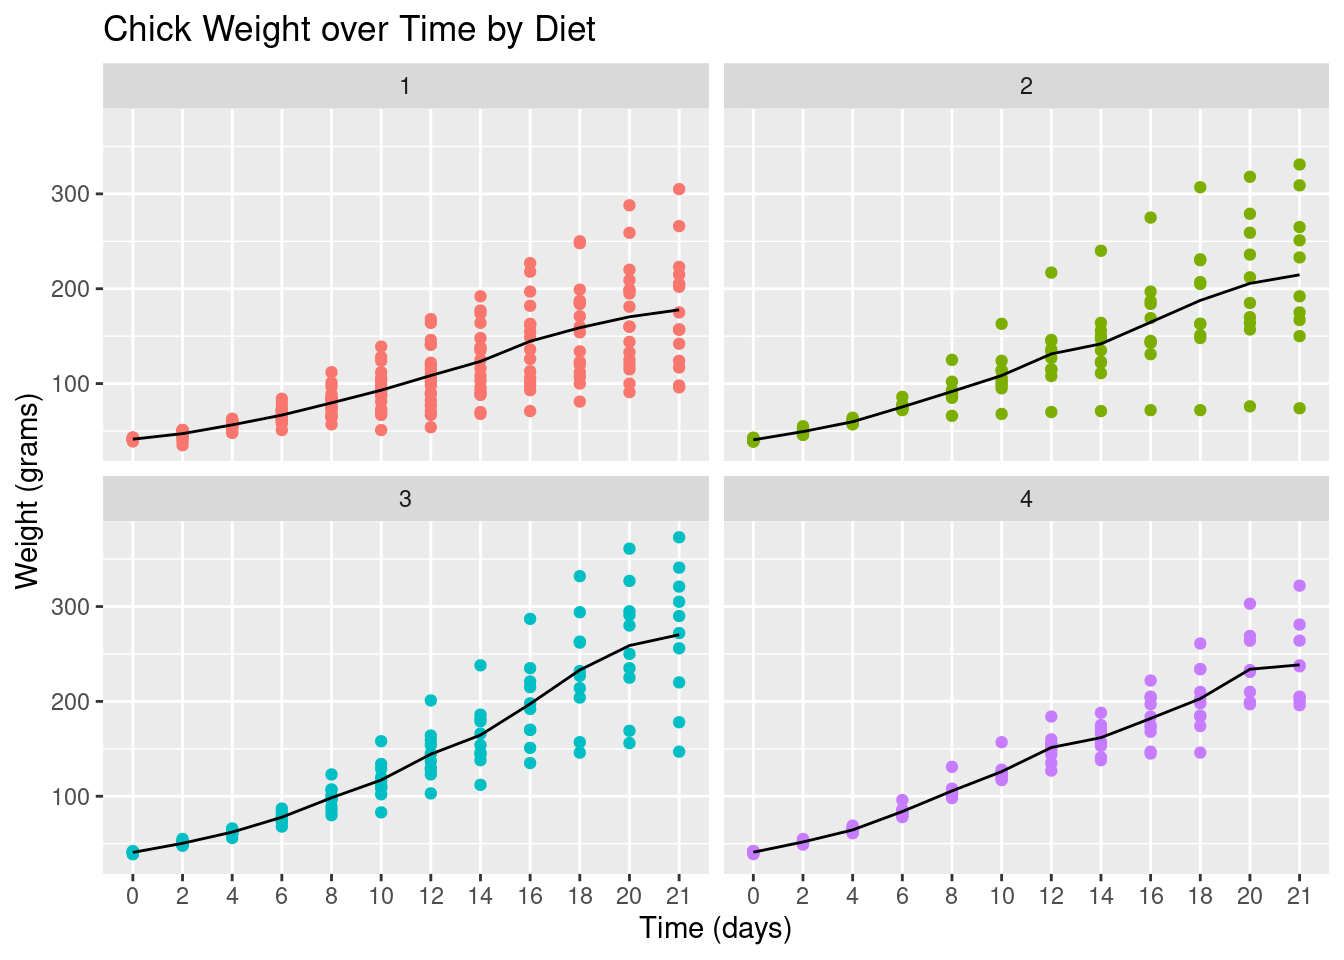
\includegraphics{01-Introduction-to-R_files/figure-latex/finalPlot-1.pdf}

\hypertarget{tidyverse-data-wrangling-basics}{%
\subsection{Tidyverse: Data Wrangling Basics}\label{tidyverse-data-wrangling-basics}}

In this section we will learn how to wrangle (manipulate) datasets using the \texttt{tidyverse}
package. Let's start with the \texttt{mutate()}, \texttt{select()}, \texttt{rename()}, \texttt{filter()} and \texttt{arrange()}
functions.

\hfill\break

\texttt{mutate()}: Adds a new variable (column) or modifies an existing one. We already used this above to create
factor variables.

\begin{Shaded}
\begin{Highlighting}[]
\CommentTok{\# Added a column}
\NormalTok{CWm1 }\OtherTok{\textless{}{-}} \FunctionTok{mutate}\NormalTok{(CW, }\AttributeTok{weightKg =}\NormalTok{ weight}\SpecialCharTok{/}\DecValTok{1000}\NormalTok{)}
\NormalTok{CWm1}
\end{Highlighting}
\end{Shaded}

\begin{verbatim}
## # A tibble: 578 x 5
##   Chick Diet  Time  weight weightKg
##   <dbl> <fct> <fct>  <dbl>    <dbl>
## 1    18 1     0         39    0.039
## 2    18 1     2         35    0.035
## 3    16 1     0         41    0.041
## # ... with 575 more rows
\end{verbatim}

\begin{Shaded}
\begin{Highlighting}[]
\CommentTok{\# Modify an existing column}
\NormalTok{CWm2 }\OtherTok{\textless{}{-}} \FunctionTok{mutate}\NormalTok{(CW, }\AttributeTok{Diet =} \FunctionTok{str\_c}\NormalTok{(}\StringTok{"Diet "}\NormalTok{, Diet))}
\NormalTok{CWm2}
\end{Highlighting}
\end{Shaded}

\begin{verbatim}
## # A tibble: 578 x 4
##   Chick Diet   Time  weight
##   <dbl> <chr>  <fct>  <dbl>
## 1    18 Diet 1 0         39
## 2    18 Diet 1 2         35
## 3    16 Diet 1 0         41
## # ... with 575 more rows
\end{verbatim}

\hfill\break

\texttt{select()}: Keeps, drops or reorders variables.

\begin{Shaded}
\begin{Highlighting}[]
\CommentTok{\# Drop the weight variable from CWm1 using minus}
\FunctionTok{select}\NormalTok{(CWm1, }\SpecialCharTok{{-}}\NormalTok{weight)}
\end{Highlighting}
\end{Shaded}

\begin{verbatim}
## # A tibble: 578 x 4
##   Chick Diet  Time  weightKg
##   <dbl> <fct> <fct>    <dbl>
## 1    18 1     0        0.039
## 2    18 1     2        0.035
## 3    16 1     0        0.041
## # ... with 575 more rows
\end{verbatim}

\begin{Shaded}
\begin{Highlighting}[]
\CommentTok{\# Keep variables Time, Diet and weightKg}
\FunctionTok{select}\NormalTok{(CWm1, Chick, Time, Diet, weightKg)}
\end{Highlighting}
\end{Shaded}

\begin{verbatim}
## # A tibble: 578 x 4
##   Chick Time  Diet  weightKg
##   <dbl> <fct> <fct>    <dbl>
## 1    18 0     1        0.039
## 2    18 2     1        0.035
## 3    16 0     1        0.041
## # ... with 575 more rows
\end{verbatim}

\hfill\break

\texttt{rename()}: Renames variables whilst keeping all variables.

\begin{Shaded}
\begin{Highlighting}[]
\FunctionTok{rename}\NormalTok{(CW, }\AttributeTok{Group =}\NormalTok{ Diet, }\AttributeTok{Weight =}\NormalTok{ weight)}
\end{Highlighting}
\end{Shaded}

\begin{verbatim}
## # A tibble: 578 x 4
##   Chick Group Time  Weight
##   <dbl> <fct> <fct>  <dbl>
## 1    18 1     0         39
## 2    18 1     2         35
## 3    16 1     0         41
## # ... with 575 more rows
\end{verbatim}

\hfill\break

\texttt{filter()}: Keeps or drops observations (rows).

\begin{Shaded}
\begin{Highlighting}[]
\FunctionTok{filter}\NormalTok{(CW, Time}\SpecialCharTok{==}\DecValTok{21} \SpecialCharTok{\&}\NormalTok{ weight}\SpecialCharTok{\textgreater{}}\DecValTok{300}\NormalTok{)}
\end{Highlighting}
\end{Shaded}

\begin{verbatim}
## # A tibble: 8 x 4
##   Chick Diet  Time  weight
##   <dbl> <fct> <fct>  <dbl>
## 1     7 1     21       305
## 2    29 2     21       309
## 3    21 2     21       331
## # ... with 5 more rows
\end{verbatim}

For comparing values in vectors use: \texttt{\textless{}} (less than), \texttt{\textgreater{}} (greater than), \texttt{\textless{}=}
(less than and equal to), \texttt{\textgreater{}=} (greater than and equal to), \texttt{==} (equal to) and \texttt{!=}
(not equal to). These can be combined logically using \texttt{\&} (and) and \texttt{\textbar{}} (or).

\hfill\break

\texttt{arrange()}: Changes the order of the observations.

\begin{Shaded}
\begin{Highlighting}[]
\FunctionTok{arrange}\NormalTok{(CW, Chick, Time)}
\end{Highlighting}
\end{Shaded}

\begin{verbatim}
## # A tibble: 578 x 4
##   Chick Diet  Time  weight
##   <dbl> <fct> <fct>  <dbl>
## 1     1 1     0         42
## 2     1 1     2         51
## 3     1 1     4         59
## # ... with 575 more rows
\end{verbatim}

\begin{Shaded}
\begin{Highlighting}[]
\FunctionTok{arrange}\NormalTok{(CW, }\FunctionTok{desc}\NormalTok{(weight))}
\end{Highlighting}
\end{Shaded}

\begin{verbatim}
## # A tibble: 578 x 4
##   Chick Diet  Time  weight
##   <dbl> <fct> <fct>  <dbl>
## 1    35 3     21       373
## 2    35 3     20       361
## 3    34 3     21       341
## # ... with 575 more rows
\end{verbatim}

What does the \texttt{desc()} do? Try using \texttt{desc(Time)}.

\hypertarget{the-pipe-operator}{%
\subsection{\texorpdfstring{The pipe operator \texttt{\%\textgreater{}\%}}{The pipe operator \%\textgreater\%}}\label{the-pipe-operator}}

In reality you will end up doing multiple data wrangling steps that you want to save.
The pipe operator \texttt{\%\textgreater{}\%} makes your code nice and readable:

\begin{Shaded}
\begin{Highlighting}[]
\NormalTok{CW21 }\OtherTok{\textless{}{-}}\NormalTok{ CW }\SpecialCharTok{\%\textgreater{}\%} 
  \FunctionTok{filter}\NormalTok{(Time }\SpecialCharTok{\%in\%} \FunctionTok{c}\NormalTok{(}\DecValTok{0}\NormalTok{, }\DecValTok{21}\NormalTok{)) }\SpecialCharTok{\%\textgreater{}\%} 
  \FunctionTok{rename}\NormalTok{(}\AttributeTok{Weight =}\NormalTok{ weight) }\SpecialCharTok{\%\textgreater{}\%} 
  \FunctionTok{mutate}\NormalTok{(}\AttributeTok{Group =} \FunctionTok{factor}\NormalTok{(}\FunctionTok{str\_c}\NormalTok{(}\StringTok{"Diet "}\NormalTok{, Diet))) }\SpecialCharTok{\%\textgreater{}\%} 
  \FunctionTok{select}\NormalTok{(Chick, Group, Time, Weight) }\SpecialCharTok{\%\textgreater{}\%} 
  \FunctionTok{arrange}\NormalTok{(Chick, Time) }
\NormalTok{CW21}
\end{Highlighting}
\end{Shaded}

\begin{verbatim}
## # A tibble: 95 x 4
##   Chick Group  Time  Weight
##   <dbl> <fct>  <fct>  <dbl>
## 1     1 Diet 1 0         42
## 2     1 Diet 1 21       205
## 3     2 Diet 1 0         40
## # ... with 92 more rows
\end{verbatim}

Hint: To understand the code above we should read the pipe operator \texttt{\%\textgreater{}\%} as ``then''.

\begin{quote}
Create a new dataset (object) called \texttt{CW21} using dataset \texttt{CW} \textbf{\emph{then}}
keep the data for days 0 and 21 \textbf{\emph{then}} rename variable \texttt{weight} to \texttt{Weight}
\textbf{\emph{then}} create a variable called \texttt{Group} \textbf{\emph{then}} keep variables \texttt{Chick},
\texttt{Group}, \texttt{Time} and \texttt{Weight} and \textbf{\emph{then}} finally arrange the data by
variables \texttt{Chick} and \texttt{Time}.
\end{quote}

This is the same code:

\begin{Shaded}
\begin{Highlighting}[]
\NormalTok{CW21 }\OtherTok{\textless{}{-}}\NormalTok{ CW }\SpecialCharTok{\%\textgreater{}\%} 
  \FunctionTok{filter}\NormalTok{(., Time }\SpecialCharTok{\%in\%} \FunctionTok{c}\NormalTok{(}\DecValTok{0}\NormalTok{, }\DecValTok{21}\NormalTok{)) }\SpecialCharTok{\%\textgreater{}\%} 
  \FunctionTok{rename}\NormalTok{(., }\AttributeTok{Weight =}\NormalTok{ weight) }\SpecialCharTok{\%\textgreater{}\%} 
  \FunctionTok{mutate}\NormalTok{(., }\AttributeTok{Group=}\FunctionTok{factor}\NormalTok{(}\FunctionTok{str\_c}\NormalTok{(}\StringTok{"Diet "}\NormalTok{,Diet))) }\SpecialCharTok{\%\textgreater{}\%} 
  \FunctionTok{select}\NormalTok{(., Chick, Group, Time, Weight) }\SpecialCharTok{\%\textgreater{}\%} 
  \FunctionTok{arrange}\NormalTok{(., Chick, Time) }
\end{Highlighting}
\end{Shaded}

The pipe operator, \texttt{\%\textgreater{}\%}, replaces the dots (\texttt{.}) with whatever is returned from code
preceding it. For example, the dot in \texttt{filter(.,\ Time\ \%in\%\ c(0,\ 21))} is replaced by
\texttt{CW}. The output of the \texttt{filter(...)} then replaces the dot in
\texttt{rename(.,\ Weight\ =\ weight)} and so on. Think of it as a data assembly line with
each function doing its thing and passing it to the next.

\hypertarget{the-group_by-function}{%
\subsection{\texorpdfstring{The \texttt{group\_by()} function}{The group\_by() function}}\label{the-group_by-function}}

From the data visualizations above we concluded that the diet 3 has the highest mean
and diet 4 the least variation. In this section, we will quantify the effects of the
diets using \textbf{summmary statistics}. We start by looking at the number of observations
and the mean by \textbf{diet} and \textbf{time}.

\begin{Shaded}
\begin{Highlighting}[]
\NormalTok{mnsdCW }\OtherTok{\textless{}{-}}\NormalTok{ CW }\SpecialCharTok{\%\textgreater{}\%} 
  \FunctionTok{group\_by}\NormalTok{(Diet, Time) }\SpecialCharTok{\%\textgreater{}\%} 
  \FunctionTok{summarise}\NormalTok{(}\AttributeTok{N =} \FunctionTok{n}\NormalTok{(), }\AttributeTok{Mean =} \FunctionTok{mean}\NormalTok{(weight)) }\SpecialCharTok{\%\textgreater{}\%} 
  \FunctionTok{arrange}\NormalTok{(Diet, Time)}
\end{Highlighting}
\end{Shaded}

\begin{verbatim}
## `summarise()` has grouped output by 'Diet'. You can override using the `.groups` argument.
\end{verbatim}

\begin{Shaded}
\begin{Highlighting}[]
\NormalTok{mnsdCW}
\end{Highlighting}
\end{Shaded}

\begin{verbatim}
## # A tibble: 48 x 4
## # Groups:   Diet [4]
##   Diet  Time      N  Mean
##   <fct> <fct> <int> <dbl>
## 1 1     0        20  41.4
## 2 1     2        20  47.2
## 3 1     4        19  56.5
## # ... with 45 more rows
\end{verbatim}

For each distinct combination of \texttt{Diet} and \texttt{Time}, the chick weight data is summarized
into the number of observations (\texttt{N}) and the mean (\texttt{Mean}) of \texttt{weight}.

\textbf{Further summaries:} Let's also calculate the standard deviation, median, minimum and maximum values but only
at days 0 and 21.

\begin{Shaded}
\begin{Highlighting}[]
\NormalTok{sumCW }\OtherTok{\textless{}{-}}\NormalTok{  CW }\SpecialCharTok{\%\textgreater{}\%} 
  \FunctionTok{filter}\NormalTok{(Time }\SpecialCharTok{\%in\%} \FunctionTok{c}\NormalTok{(}\DecValTok{0}\NormalTok{, }\DecValTok{21}\NormalTok{)) }\SpecialCharTok{\%\textgreater{}\%} 
  \FunctionTok{group\_by}\NormalTok{(Diet, Time) }\SpecialCharTok{\%\textgreater{}\%} 
  \FunctionTok{summarise}\NormalTok{(}\AttributeTok{N =} \FunctionTok{n}\NormalTok{(),}
            \AttributeTok{Mean =} \FunctionTok{mean}\NormalTok{(weight),}
            \AttributeTok{SD =} \FunctionTok{sd}\NormalTok{(weight),}
            \AttributeTok{Median =} \FunctionTok{median}\NormalTok{(weight),}
            \AttributeTok{Min =} \FunctionTok{min}\NormalTok{(weight),}
            \AttributeTok{Max =} \FunctionTok{max}\NormalTok{(weight)) }\SpecialCharTok{\%\textgreater{}\%} 
  \FunctionTok{arrange}\NormalTok{(Diet, Time)}
\end{Highlighting}
\end{Shaded}

\begin{verbatim}
## `summarise()` has grouped output by 'Diet'. You can override using the `.groups` argument.
\end{verbatim}

\begin{Shaded}
\begin{Highlighting}[]
\NormalTok{sumCW}
\end{Highlighting}
\end{Shaded}

\begin{verbatim}
## # A tibble: 8 x 8
## # Groups:   Diet [4]
##   Diet  Time      N  Mean     SD Median   Min   Max
##   <fct> <fct> <int> <dbl>  <dbl>  <dbl> <dbl> <dbl>
## 1 1     0        20  41.4  0.995   41      39    43
## 2 1     21       16 178.  58.7    166      96   305
## 3 2     0        10  40.7  1.49    40.5    39    43
## # ... with 5 more rows
\end{verbatim}

Let's make the summaries ``prettier'', say, for a report or publication.

\begin{Shaded}
\begin{Highlighting}[]
\FunctionTok{library}\NormalTok{(}\StringTok{"knitr"}\NormalTok{) }\CommentTok{\# to use the kable() function}
\NormalTok{prettySumCW }\OtherTok{\textless{}{-}}\NormalTok{ sumCW }\SpecialCharTok{\%\textgreater{}\%} 
 \FunctionTok{mutate}\NormalTok{(}\StringTok{\textasciigrave{}}\AttributeTok{Mean (SD)}\StringTok{\textasciigrave{}} \OtherTok{=} \FunctionTok{str\_c}\NormalTok{(}\FunctionTok{format}\NormalTok{(Mean, }\AttributeTok{digits=}\DecValTok{1}\NormalTok{),}
           \StringTok{" ("}\NormalTok{, }\FunctionTok{format}\NormalTok{(SD, }\AttributeTok{digits=}\DecValTok{2}\NormalTok{), }\StringTok{")"}\NormalTok{)) }\SpecialCharTok{\%\textgreater{}\%} 
 \FunctionTok{mutate}\NormalTok{(}\AttributeTok{Range =} \FunctionTok{str\_c}\NormalTok{(Min, }\StringTok{" {-} "}\NormalTok{, Max)) }\SpecialCharTok{\%\textgreater{}\%} 
 \FunctionTok{select}\NormalTok{(Diet, Time, N, }\StringTok{\textasciigrave{}}\AttributeTok{Mean (SD)}\StringTok{\textasciigrave{}}\NormalTok{, Median, Range) }\SpecialCharTok{\%\textgreater{}\%}
 \FunctionTok{arrange}\NormalTok{(Diet, Time) }\SpecialCharTok{\%\textgreater{}\%} 
 \FunctionTok{kable}\NormalTok{(}\AttributeTok{format =} \StringTok{"latex"}\NormalTok{)}
\NormalTok{prettySumCW}
\end{Highlighting}
\end{Shaded}

\begin{tabular}{l|l|r|l|r|l}
\hline
Diet & Time & N & Mean (SD) & Median & Range\\
\hline
1 & 0 & 20 & 41 ( 0.99) & 41.0 & 39 - 43\\
\hline
1 & 21 & 16 & 178 (58.70) & 166.0 & 96 - 305\\
\hline
2 & 0 & 10 & 41 ( 1.5) & 40.5 & 39 - 43\\
\hline
2 & 21 & 10 & 215 (78.1) & 212.5 & 74 - 331\\
\hline
3 & 0 & 10 & 41 ( 1) & 41.0 & 39 - 42\\
\hline
3 & 21 & 10 & 270 (72) & 281.0 & 147 - 373\\
\hline
4 & 0 & 10 & 41 ( 1.1) & 41.0 & 39 - 42\\
\hline
4 & 21 & 9 & 239 (43.3) & 237.0 & 196 - 322\\
\hline
\end{tabular}

\textbf{Interpretation:}
This summary table offers the same interpretation as before, namely that diet 3 has the
highest mean and median weights at day 21 but a higher variation than group 4.
However it should be noted that at day 21, diet 1 lost 4 chicks from 20 that started
and diet 4 lost 1 from 10. This could be a sign of some health related issues.

\hypertarget{further-links}{%
\section{Further Links}\label{further-links}}

\hypertarget{further-r-intros}{%
\subsection{Further R-Intros}\label{further-r-intros}}

\begin{itemize}
\item
  \url{https://eddelbuettel.github.io/gsir-te/Getting-Started-in-R.pdf}
\item
  \url{https://www.datacamp.com/courses/free-introduction-to-r}
\item
  \url{https://swcarpentry.github.io/r-novice-gapminder/}
\item
  \url{https://support.rstudio.com/hc/en-us/articles/200526207-Using-Projects}
\end{itemize}

\hypertarget{version-control-gitgithub}{%
\subsection{Version Control (Git/GitHub)}\label{version-control-gitgithub}}

\begin{itemize}
\item
  \url{https://support.rstudio.com/hc/en-us/articles/200532077-Version-Control-with-Git-and-SVN}
\item
  \url{http://happygitwithr.com/}
\item
  \url{https://www.gitkraken.com/}
\end{itemize}

\hypertarget{r-ladies}{%
\subsection{R-Ladies}\label{r-ladies}}

\begin{itemize}
\tightlist
\item
  \url{https://rladies.org/}
\end{itemize}

\hypertarget{estimation-theory}{%
\chapter{Estimation Theory}\label{estimation-theory}}

\hypertarget{bias-variance-and-mse}{%
\section{Bias, Variance and MSE}\label{bias-variance-and-mse}}

Given a sample \(X_1,\dots,X_n\) consider an estimator \(\widehat{\theta}_n\equiv\widehat{\theta}(X_1,\dots,X_n)\) of a real-valued parameter \(\theta\in\Omega\subset\mathbb{R}\).

The distribution of any estimator of course depends on the true parameter vector \(\theta\), i.e., more precisely, \[\widehat{\theta}_n\equiv \widehat{\theta}(X_1,\dots,X_n;\theta).\]
This dependence is usually not explicitly written, but all properties of estimators discussed below have to hold for all possible parameter values \(\theta\in\Omega\). This will go without saying.

\hfill\break

Statistical inference requires to assess the accuracy of an estimator.

\hfill\break

The \textbf{bias} of an estimator is defined by
\[\textrm{Bias}(\widehat{\theta}_n)=E(\widehat{\theta}_n)-\theta\]
An estimator is called \textbf{unbiased} if \(E(\widehat{\theta}_n)=\theta\) and hence \(\textrm{Bias}(\widehat{\theta}_n)=0\) (for all possible \(\theta\in\Omega\)).

\hfill\break

The \textbf{variance} of an estimator is given by
\[\textrm{var}(\widehat{\theta}_n)=E\left((\widehat{\theta}_n-E(\widehat{\theta}_n))^2\right).\]

\hfill\break

Performance of an estimator is most frequently evaluated with respect to the \textbf{quadratic loss} (also
called \(L_2\) loss)
\[(\widehat{\theta}_n-\theta)^2.\]
The corresponding risk is the \textbf{Mean Squared Error (MSE)}
\[E\left((\widehat{\theta}_n-\theta)^2\right)=\textrm{Bias}(\widehat{\theta}_n)^2+\textrm{var}(\widehat{\theta}_n)\]
For an unbiased estimator the mean squared error is obviously equal to the variance of the estimator.

\hfill\break

\textbf{Example:} Assume an i.i.d. sample \(X_1,\dots,X_n\) with mean \(\mu=E(X_i)\) and variance \(\sigma^2=\textrm{var}(X_i)<\infty\).

\begin{itemize}
\tightlist
\item
  The sample mean \(\bar X\) is an unbiased estimator of the true mean \(\mu\), since the equation
  \[E(\bar X)=\mu\]
  holds for any possible value of the true mean \(\mu\).
\item
  The variance of the estimator \(\bar X\) is given by
  \[\textrm{var}(\bar X)=\sigma^2/n\]
\item
  The mean squared error of the estimator \(\bar X\) is given by
  \[E\left((\bar X-\mu)^2\right)=\textrm{var}(\bar X)=\sigma^2/n\]
\end{itemize}

\hypertarget{consistency-of-estimators}{%
\section{Consistency of Estimators}\label{consistency-of-estimators}}

Asymptotic theory is concerned with theoretical results valid for ``large sample sizes''. Important keywords of asymptotic theory are:

\begin{itemize}
\tightlist
\item
  consistency
\item
  rates of convergence
\item
  asymptotic distributions
\end{itemize}

They all rely on elaborated concepts on the stochastic convergence of random variables.

\hfill\break

\textbf{Stochastic convergence.}
Let \(\{Z_n\}_{n=1,2,3,\dots}\) be a sequence of \textbf{random variables}. Mathematically, there are different kinds of convergence of
\(\{Z_n\}\) to a fixed value \(c\). The three most important are:

\begin{itemize}
\tightlist
\item
  Convergence in probability (abbreviated \(Z_n\to_P c\)):
  \[\lim_{n\to\infty} P\left(|Z_n-c|>\epsilon\right)=0\quad\hbox{ for all }\quad\epsilon>0\]
\item
  Almost sure convergence (abbreviated \(Z_n\to_{a.s.} c\)):
  \[P\left(\lim_{n\to\infty} Z_n=c\right)=1\]
\item
  Convergence in quadratic mean (abbreviated \(Z_n\to_{q.m.} c\)):
  \[\lim_{n\to\infty} E\left((Z_n-c)^2\right)=0\]
\end{itemize}

Note that:

\begin{itemize}
\tightlist
\item
  \(Z_n\to_{a.s.} c\) implies \(Z_n\to_P c\)
\item
  \(Z_n\to_{q.m.} c\) implies \(Z_n\to_P c\)
\end{itemize}

\hfill\break

\textbf{Consistency of estimators.} Based on a sample \(X_1,\dots,X_n\) let \(\hat\theta_n\equiv\theta_n(X_1,\dots,X_n)\) be an estimator of an unknown parameter \(\theta\).

\begin{itemize}
\tightlist
\item
  \(\hat\theta_n\) is called ``weakly consistent'' if
  \[\hat{\theta}_n\to_{P} \theta\quad \hbox{ as }\quad n\to\infty \]
\item
  \(\hat\theta_n\) is called ``strongly consistent'' if
  \[\hat{\theta}_n\to_{a.s.} \theta\quad \hbox{ as }\quad n\to\infty \]
\end{itemize}

\hfill\break

\textbf{Remark:} For most statistical estimation problems it is usually possible to define many different estimators. The real problem is to find a good estimator which approximates the true parameter \(\theta\) with the maximal possible accuracy. Consistency is generally seen as a necessary condition which has to be satisfied by any reasonable estimator. In econometric practice usually only weak consistency is derived which generally follows from weak \href{https://www.statlect.com/asymptotic-theory/law-of-large-numbers}{\textbf{laws of large numbers}}.

\hfill\break

\textbf{Example:} Assume again an i.i.d. sample \(X_1,\dots,X_n\) with mean \(\mu=E(X_i)\) and variance \(\sigma^2=\textrm{var}(X_i)<\infty\). As stated above we then have
\[E\left((\bar X-\mu)^2\right)=\textrm{var}(\bar X)=\sigma^2/n\rightarrow 0 \quad \text{as } n\rightarrow\infty.\]
Therefore, \(\bar X \to_{q.m.} \mu\). The latter implies that \(\bar X \to_{P} \mu\), i.e.~\(\bar X\) is a (weakly) consistent estimator of \(\mu\).

\hypertarget{rates-of-convergence}{%
\section{Rates of Convergence}\label{rates-of-convergence}}

Rates of convergence quantify the (stochastic) order of magnitude of an estimation error in dependence of the
sample size \(n\). This order of magnitude is usually represented using the symbols: \(O_P\) and \(o_P\).

\hfill\break

Let \(\{Z_n\}_{n=1,2,3,\dots}\) be a sequence of random variables, and let \(\{c_n\}_{n=1,2,3,\dots}\) be a sequence of positive (deterministic) numbers.

\begin{itemize}
\tightlist
\item
  We will write \(Z_n=O_p(c_n)\) if for any \(\epsilon>0\) there exist numbers \(0<M<\infty\) and \(m\) such that
  \[P(|Z_n|\ge M\cdot c_n)\leq\epsilon\quad\hbox{ for all }\quad n\geq m.\]
\item
  We will write \(Z_n=o_p(c_n)\) if
  \[\lim_{n\to\infty} P(|Z_n|\geq\epsilon\cdot c_n)=0\quad\hbox{ for all }\quad \epsilon>0.\]
\item
  With \(c_n=1\) for all \(n\), \(Z_n=O_p(1)\) means that the sequence \(\{Z_n\}\) is \textbf{stochastically bounded}. I.e., for any \(\epsilon>0\) there exist number \(0<M<\infty\) and \(m\) such that
  \[P(|Z_n|\geq M)\leq\epsilon\quad\hbox{ for all }\quad n\geq m.\]
\item
  With \(c_n=1\) for all \(n\), \(Z_n=o_P(1)\) is equivalent to \(Z_n\to_{P} 0\), i.e., \(Z_n\) \textbf{converges in probability to zero}.
\end{itemize}

Note that:

\begin{itemize}
\tightlist
\item
  \(Z_n=O_p(c_n)\) is equivalent to \(Z_n/c_n=O_p(1)\)
\item
  \(Z_n=o_p(c_n)\) is equivalent to \(Z_n/c_n=o_p(1)\)
\end{itemize}

\hfill\break

\textbf{Definition:} An estimator \(\hat\theta\equiv\hat\theta_n\) of a parameter \(\theta\) possesses the
\textbf{rate of convergence} \(n^{-r}\) if and only if \(r\) is the \emph{largest positive number} with the property that
\[|\hat\theta_n-\theta|=O_P(n^{-r}).\]

The rate of convergence quantifies how fast the estimation error decreases when increasing the sample size \(n\).

\hfill\break

\textbf{Unbiased estimators:} Let \(\hat\theta_n\) be an \emph{unbiased} estimator of an unknown parameter \(\theta\) satisfying \(\textrm{var}(\hat\theta_n)=C n^{-1}\) for some \(0<C<\infty\). Then \(\hat\theta_n\) possesses the rate of convergence \(n^{-1/2}\). This is a consequence of the \href{https://www.statlect.com/fundamentals-of-probability/Chebyshev-inequality}{Chebyshev inequality}.

\hfill\break

\textbf{Chebyshev inequality:} If \(Z\) denotes a random variable with mean \(\mu\) and variance \(\sigma^2\), then
\[P\left(|X-\mu|> \sigma \cdot m\right)\le \frac{1}{m^2}\quad\hbox{ for all }\quad m>0\]
\[\Rightarrow
P\left(|\hat\theta_n-\theta|> n^{-1/2}\sqrt{C} \cdot
\frac{1}{\sqrt{\epsilon}}\right)\leq \epsilon \quad\hbox{ for all }\quad\epsilon>0\]

\hfill\break

\textbf{Example:} Assume an i.i.d. sample \(X_1,\dots,X_n\) with mean \(\mu=E(X_i)\) and variance \(\sigma^2=\textrm{var}(X_i)<\infty\). The sample mean \(\bar X\) (\(\equiv \bar X_n\)) is an unbiased estimator of \(\mu\) with variance \(\textrm{var}(\bar X)=\sigma^2/n\).
For large \(n\) we have by the central limit theorem that approximately \(\sqrt{n}(\bar X-\mu)\sim N(0,\sigma^2)\). Therefore, for example:

\begin{itemize}
\tightlist
\item
  with \(\epsilon=0.05\) we obtain
  \[P\left(|\bar X_n-\mu|\ge 1.96\sigma\cdot n^{-1/2}\right)=0.05\]
\item
  with \(\epsilon=0.01\) we obtain
  \[P\left(|\bar X_n-\mu|\ge 2.64\sigma\cdot n^{-1/2}\right)=0.01.\]
\end{itemize}

Generalizing this argument for all possible \(\epsilon>0\) we can conclude that
\(\bar X-\mu=O_P(n^{-1/2})\). On the other hand for any \(r>1/2\) we have \(n^{-r}/n^{-1/2}\rightarrow 0\) as \(n\rightarrow \infty\). Hence, for any constant \(c>0\)

\begin{align*}
 &P\left(|\bar X_n-\mu|\geq c\sigma\cdot n^{-r}\right)=\\
=&P\left(|\bar X_n-\mu|\ge (c\sigma\cdot n^{-1/2})\cdot\frac{n^{-r}}{n^{-1/2}}\right)\rightarrow 1 \quad\text{as}\quad n\rightarrow \infty.
\end{align*}

Therefore \(n^{-1/2}\) is the \textbf{rate of convergence} of \(\bar X\).

\hfill\break

Note that:

\begin{itemize}
\tightlist
\item
  Maximum-likelihood estimators of an unknown parameter usually possess the rate of convergence \(n^{-1/2}\) (there are exceptions!).
\item
  The situation is different, for instance, in nonparametric curve estimation problems. For example kernel estimators (of a density or regression function) only achieve the rate of convergence \(n^{-2/5}\).
\item
  The rate of convergence is an important criterion for selecting the best possible estimator for a given problem. For most parametric problems it is well known that the optimal (i.e.~fastest possible) convergence rate is \(n^{-1/2}\). In nonparametric regression or density estimation the optimal convergence rate is only \(n^{-2/5}\), if the underlying function is twice continuously differentiable.
\end{itemize}

\hfill\break

\(O_P\)-rules:

\begin{itemize}
\tightlist
\item
  We have
  \[Z_n\rightarrow_P Z \qquad \text{if and only if }\qquad Z_n=Z+o_p(1)\]
  This follows from \(Z_n=Z+(Z_n-Z)\) and \(Z_n-Z\rightarrow_P 0\).
\end{itemize}

\hfill\break

\begin{itemize}
\tightlist
\item
  If \(Z_n=O_P(n^{-\delta})\) for some \(\delta>0\), then \(Z_n=o_P(1)\)
\end{itemize}

\hfill\break

\begin{itemize}
\tightlist
\item
  If \(Z_n=O_P(r_n)\), then \(Z_n^\delta=O_P(r_n^\delta)\) for any \(\delta>0\). Similarly,
  \(Z_n=o_P(r_n)\) implies \(Z_n^\delta=o_P(r_n^\delta)\) for any \(\delta>0\).
\end{itemize}

\hfill\break

\begin{itemize}
\tightlist
\item
  If \(Z_n=O_P(r_n)\) and \(V_n=O_P(s_n)\), then
  \begin{align*}
  Z_n+V_n & =O_P(\max\{r_n,s_n\})\\
  Z_nV_n &  =O_P(r_ns_n)
  \end{align*}
\end{itemize}

\hfill\break

\begin{itemize}
\tightlist
\item
  If \(Z_n=o_P(r_n)\) and \(V_n=O_P(s_n)\), then \(Z_nV_n=o_P(r_n s_n)\)
\end{itemize}

\hfill\break

\begin{itemize}
\tightlist
\item
  If \(E(|Z_n|^k)=O(r_n)\), then \(Z_n=O_p(|r_n|^{1/k})\) for \(k=1,2,3,\dots\)
\end{itemize}

\hypertarget{asymptotic-distributions}{%
\section{Asymptotic Distributions}\label{asymptotic-distributions}}

The practically most important version of stochastic convergence is convergence in distribution. Knowledge about the ``asymptotic distribution'' of an estimator allows to construct confidence intervals and tests.

\hfill\break

\textbf{Definition:} Let \(Z_n\) be a sequence of random variables with corresponding distribution functions \(G_n\). Then \(Z_n\) \textbf{converges in distribution} to a random variable \(Z\) with distribution function \(G\), if
\[G_n(x)\to G(x)\quad\hbox{ as }\quad n\to\infty \]
at all continuity points \(x\) of \(G\) (abbreviated: \(Z_n\to_L Z\) or \(Z_n\to_L G\) or ``\(\to_D\)'' instead of ``\(\to_L\)'').

\hfill\break

In a vast majority of practically important situation the limiting distribution is the normal distribution. One then speaks of \textbf{asymptotic normality}. Asymptotic normality is usually a consequence of \href{https://www.statlect.com/asymptotic-theory/central-limit-theorem\%5D}{central limit theorems}. The simplest result in this direction is the central limit theorem of Lindeberg-Levy.

\hfill\break

\textbf{Theorem (Lindeberg-Levy)} Let \(Z_1,Z_2,\dots\) be a sequence of i.i.d. random variables with
finite mean \(\mu\) and variance \(\sigma^2<\infty\). Then
\[\sqrt{n}\left(\frac{1}{n} \sum_{i=1}^n Z_i -\mu\right)\rightarrow_L N(0,\sigma^2).\]

\hfill\break

\textbf{Example:} Let \(X_1,\dots,X_n\) be independent random variables
with \(E(X_i)=\mu\), \(Var(X_i)=\sigma^2\). Then the central limit theorem of Lindeberg-Levy implies that
\[\sqrt{n}(\bar X -\mu ) \to_L N(0,\sigma^2)\quad\text{ or equivalently }\quad
\frac{\sqrt{n}(\bar X -\mu )}{\sigma}\to_L N(0,1).\]
We can conclude that \(\bar X\) is an ``asymptotically normal estimator'' of \(\mu\). If \(n\) is sufficiently large, then \(\bar X\) is approximatively normal with mean \(\mu\) and variance \(\sigma^2/n\). Frequently used notations:

\begin{itemize}
\tightlist
\item
  \(\bar X\sim AN(\mu,\sigma^2/n)\)
\item
  \(\bar X\overset{a}{\sim}N(\mu,\sigma^2/n)\)
\end{itemize}

\hfill\break

Most estimators \(\hat\theta_n\) used in parametric and nonparametric statistics are asymptotically normal. In parametric problems (with rate of convergence \(n^{-1/2}\)) one usually obtains
\[\sqrt{n}(\hat\theta_n -\theta )\to_L N(0,v^2),\]
where \(v^2\) is the asymptotic variance of the estimator (often, but not necessarily, \(v^2=\lim_{n\to\infty} n\cdot\textrm{var}(\hat\theta_n)\)).

\hfill\break

\textbf{Multivariate generalization:} The above concepts are easily generalized to estimators \(\hat\theta_n\) of a multivariate parameter vector \(\theta\in\mathbb{R}^p\). Consistency and rates of convergence then have to be derived separately for each element of the vector. Convergence in distribution is defined via convergence of the multivariate distribution functions. For standard estimators (e.g., maximum likelihood) in parametric problems one usually obtains
\[\sqrt{n}(\hat\theta_n -\theta )\to_L N_p(0,V),\]
where \(V\) is the asymptotic covariance matrix (usually, \(V=\lim_{n\to\infty} n\cdot\textrm{Cov}(\hat\theta_n)\)).

\hfill\break

Multivariate normality holds if and only if for any vector \(c=(c_1,\dots,c_p)'\in\mathbb{R}^p\) with \(\sum_{j=1}^p c_j^2=\Vert c\Vert_2^2=1\)
\[\sqrt{n}\left(\sum_{j=1}^p c_j (\hat\theta_{jn} -\theta_j)\right)=\sqrt{n}\left(c'\hat\theta_n-c'\theta\right)\to_L N\left(0,v_c^2\right),\]
where
\[v_c^2=c'Vc=\sum_{j=1}^p\sum_{k=1}^p c_jc_k V_{jk},\]
and where \(V_{jk}\) are the elements of the asymptotic covariance matrix \(V\).

This condition is frequently called \textbf{``Cramer-Wold device''}. Using one-dimensional central limit theorems it can be verified for any vector \(c\).

\hfill\break

\textbf{Example:} Let \(X_1=(X_{11},X_{12})',\dots,X_n=(X_{n1},X_{n2})'\) be i.i.d. two-dimensional random vectors with \(E(X_i)=\mu=(\mu_1,\mu_2)'\) and \(Cov(X_i)=\Sigma\). The Cramer-Wold device and Lindeberg-Levy's central limit theorem then imply that
\[\sqrt{n}\left(\bar X -\mu\right)\to_L N_2\left(0,\Sigma\right).\]

\hfill\break

Note that asymptotic normality usually also holds for nonparametric curve estimators with convergence rates slower than \(n^{-1/2}\).

\hypertarget{asymptotic-theory}{%
\section{Asymptotic Theory}\label{asymptotic-theory}}

Many estimation procedures in modern statistics rely on fairly general assumptions. For a given sample size \(n\) it is then often impossible to derive the exact distribution of \(\theta_n\). Necessary calculations are too complex, and finite sample distributions usually depend on unknown characteristics of the distribution of the underlying data.

\hfill\break

The goal of asymptotic theory then is to derive reasonable approximations. For \textbf{large samples} such approximations are of course very accurate, for \textbf{small samples} there may exist a considerable approximation error. Therefore, for small samples the approximation quality of asymptotic approximations is usually studied by Monte-Carlo approximations.

\hfill\break

Asymptotic theory is used in order to select an appropriate estimation procedure in complex situations. The idea is to determine the estimator which, at least for large sample sizes, provides the smallest possible estimation error. This leads to the concept of ``asymptotically efficient'' estimators.

\hfill\break

Properties of an asymptotically efficient estimator \(\theta_n\):

\begin{itemize}
\tightlist
\item
  For the estimation problem to be considered \(\theta_n\) is consistent and adopts the fastest possible rate of convergence
  (generally: \(n^{-1/2}\) in parametric statistics; \(n^{-2/5}\) can be achieved in nonparametric univariate curve estimation problems).
\item
  In most regular situations one is additionally interested in a ``best asymptotically normal'' (BAN) estimator. Assume that \(\sqrt{n}(\theta_n -\theta)\sim N(0,v^2)\). Then \(\theta_n\) is a BAN-estimator if any alternative estimator \(\tilde\theta_n\) with
  \(\sqrt{n}(\tilde\theta_n -\theta)\sim N(0,\tilde v^2)\) possesses a larger asymptotic variance, i.e.~\(\tilde v^2\geq v^2\).
\item
  \textbf{Multivariate generalization:} An estimator \(\theta_n\) with \(\sqrt{n}(\theta_n -\theta)\sim N_p(0,V)\) is best asymptotically normal if
  \[c'\tilde V c\geq c'Vc\quad\hbox{ for all }\quad c\in\mathbb{R}^p, \Vert c\Vert_2^2=1\]
  for any other estimator \(\tilde\theta_n\) satisfying \(\sqrt{n}(\tilde\theta_n -\theta)\sim N_p(0,\tilde V)\).
\end{itemize}

\hfill\break

For most estimation problems in parametric statistics maximum-likelihood estimators are best asymptotically normal.

\hypertarget{mathematical-tools}{%
\section{Mathematical tools}\label{mathematical-tools}}

\hypertarget{taylor-expansions}{%
\subsection{Taylor expansions}\label{taylor-expansions}}

Taylors' theorem: Let \(f\) be a real-valued function which is
\(k+1\) continuously differentiable in the interior of an interval \([a,b]\). Consider a point
\(x_0\in (a,b)\). For any other value \(x\in (a,b)\) there exists some \(\psi\in [x_0,x]\) such that
\[f(x)=f(x_0)+\sum_{r=1}^k \frac{1}{r!}f^{(r)}(x_0)\cdot(x-x_0)^r+\frac{1}{(k+1)!}f^{(k+1)}(\psi)\cdot(x-x_0)^{k+1}\]\\

Qualitative version of Taylors' formula:
\[f(x)=f(x_0)+\sum_{r=1}^k \frac{1}{r!}f^{(r)}(x_0)\cdot(x-x_0)^r+O((x-x_0)^{k+1})\]

\hfill\break

\textbf{Example:} Let \(f(x)=ln(x)\) und \(x_0=1\) \(\Rightarrow\) \(f'(x_0)=1\), \(f''(x_0)=-1\).

\hfill\break

First order Taylor approximation: \(f(x)=\tilde f(x)+O((x-x_0)^{2})\), where \(\tilde f(x)=x-x_0\)

\begin{itemize}
\tightlist
\item
  \(x=1.05\) \(\Rightarrow\) \(f(x)=0.04879\), \(\tilde f(x)=0.05\) and \(|f(x)-\tilde f(x)|=0.00121\)
\item
  \(x=1.1\phantom{0}\) \(\Rightarrow\) \(f(x)=0.09531\), \(\tilde f(x)=0.1\phantom{0}\) and \(|f(x)-\tilde f(x)|=0.00469\)
\item
  \(x=1.5\phantom{0}\) \(\Rightarrow\) \(f(x)=0.40546\), \(\tilde f(x)=0.5\phantom{0}\) and \(|f(x)-\tilde f(x)|=0.09454\)
\item
  \(x=2\phantom{.00}\) \(\Rightarrow\) \(f(x)=0.69315\), \(\tilde f(x)=1\phantom{.00}\) and \(|f(x)-\tilde f(x)|=0.30685\)
\end{itemize}

\hfill\break

Second order Taylor approximation: \(f(x)=\tilde f(x)+O((x-x_0)^{3})\), where \(\tilde f(x)=x-x_0-\frac{1}{2} (x-x_0)^2\)

\begin{itemize}
\tightlist
\item
  \(x=1.05\) \(\Rightarrow\) \(f(x)=0.04879\), \(\tilde f(x)=0.04875\) and \(|f(x)-\tilde f(x)|=0.00004\)
\item
  \(x=1.1\phantom{0}\) \(\Rightarrow\) \(f(x)=0.09531\), \(\tilde f(x)=0.95\phantom{000}\) and \(|f(x)-\tilde f(x)|=0.00031\)
\item
  \(x=1.5\phantom{0}\) \(\Rightarrow\) \(f(x)=0.40546\), \(\tilde f(x)=0.375\phantom{00}\) and \(|f(x)-\tilde f(x)|=0.03046\)
\item
  \(x=2\phantom{.00}\) \(\Rightarrow\) \(f(x)=0.69315\), \(\tilde f(x)=0.5\phantom{0000}\) and \(|f(x)-\tilde f(x)|=0.19315\)
\end{itemize}

\hfill\break

\textbf{Multivariate generalization:} \(x_0,x\in\mathbb{R}^p\), \(f'(x_0)\in\mathbb{R}^p\), \(f''(x_0)\) a \(p\times p\) Matrix.

First order Taylor approximation:
\[f(x)=f(x_0)+f'(x_0)\cdot(x-x_0)+O(\Vert x-x_0\Vert_2^2)\]

Second order Taylor approximation:
\[f(x)=f(x_0)+f'(x_0)\cdot(x-x_0)+\frac{1}{2} (x-x_0)^T f''(x_0)(x-x_0)+O(\Vert x-x_0\Vert_2^3)\]

\hypertarget{tools-for-deriving-asymptotic-distributions}{%
\subsection{Tools for deriving asymptotic distributions}\label{tools-for-deriving-asymptotic-distributions}}

Let \(\{W_n\}\), \(\{Z_n\}\) be sequences of random variables, then:

\begin{itemize}
\tightlist
\item
  \(Z_n=W_n+o_P(1)\quad \Leftrightarrow \quad Z_n-W_n\to_P 0\). If additionally \(W_n\to_L N(0,v^2)\) then \(Z_n\to_L N(0,v^2)\).
\item
  For any fixed constant \(c\neq 0\): If \(Z_n\to_P c\) and \(W_n\to_L N(0,v^2)\), then
  \[cW_n\to_L N(0,c^2v^2)\quad\hbox{as well as }\quad  V_n:=Z_n\cdot W_n\to_L N(0,c^2v^2).\]
  Furthermore, If \(Z_n\) and \(c\) are positive (with probability 1) then also
  \[W_n/c\to_L N(0,v^2/c^2)\quad\hbox{as well as }\quad  V_n:= W_n/Z_n\to_L N(0,v^2/c^2).\]
\item
  Multivariate generalization (\(C\), \(Z_n\) \(p\times p\) matrices; \(W_n\) \(p\)-dimensional random vectors):
  If \(Z_n\to_P C\) as well as \(W_n\to_L N_p(0,V)\), then
  \begin{align*}
  CW_n&\to_L N_p(0,CVC')\quad\hbox{as well as }\\
  V_n:=Z_n\cdot W_n&\to_L N_p(0,CVC')
  \end{align*}
\end{itemize}

\hypertarget{the-delta-method}{%
\subsection{The Delta-Method}\label{the-delta-method}}

A further tool which is frequently used in asymptotic statistics is the so-called delta-method.

\textbf{Delta-Method:} Let \(\widehat{\theta}_n\) be a sequence of estimators of a one-dimensional parameter \(\theta\) satisfying
\(n^{r} (\widehat{\theta}_n-\theta)\rightarrow_L N(0,v^2),\) and let \(g(.)\) be a real-valued function which is continuously differentiable at \(\theta\) and satisfies \(g'(\theta)\neq 0\). Then
\[n^{r} \left(g(\widehat{\theta}_n)-g(\theta)\right) \rightarrow_L  N\left(0,g'(\theta)^2v^2\right).\]

\hfill\break

\textbf{Example:} Assume an i.i.d. random sample \(X_1,\dots,X_n\) from an exponential distribution. That is, the underlying density of \(X_i\), \(i=1,\dots,n\), is given by \(f(x|\theta)=\theta\exp(-\theta x)\). We then have \(\mu:=E(X_i)=1/\theta\) as well as \(\sigma^2_X:=\textrm{var}(X_i)=1/\theta^2\). The underlying parameter \(\theta>0\) is unknown and has to be estimated from the data.

\hfill\break

The maximum-likelihood estimator of \(\theta\) is \(\hat\theta=1/\bar X\).

\hfill\break

We know that \(\sqrt{n}(\bar X-\frac{1}{\theta})\to_L N(0,\frac{1}{\theta^2})\), but what's about the distribution of \(1/\bar X\)? For this purpose the delta-method can be applied with \(g(x)=1/x\). Then \(g'(x)=-1/x^2\), \(g'(1/\theta)=-\theta^2\), and consequently
\[n^{1/2} \left(\frac{1}{\bar X}-\theta\right)=n^{1/2}\left(g\left(\bar X\right)-g\left(\frac{1}{\theta}\right)\right)\rightarrow_L N\left(0,\theta^2\right).\]

\hypertarget{statistical-hypothesis-testing}{%
\chapter{Statistical Hypothesis Testing}\label{statistical-hypothesis-testing}}

\hypertarget{hypotheses-and-test-statistics}{%
\section{Hypotheses and Test-Statistics}\label{hypotheses-and-test-statistics}}

Assume an independently and identically distributed (i.i.d.) random sample \(X_1,\dots,X_n\), where the distribution of \(X_i\), \(i=1,\dots,n\), depends on some unknown parameter \(\theta\in\Omega\), and where \(\Omega\) is some parameter space.

\hfill\break

\textbf{General Testing Problem:}

\[H_0:\theta\in\Omega_0\]
against
\[H_1:\theta\in\Omega_1\]

\(H_0\) is the null hypothesis, while \(H_1\) is the alternative. \(\Omega_0\subset\Omega\) and \(\Omega_1\subset\Omega\) are used to denote the possible values of \(\theta\) under \(H_0\) and \(H_1\). Necessarily, \(\Omega_0\cap\Omega_1=\emptyset\).

For a large number of tests we have \(\Omega\subseteq\mathbb{R}\) and the respective null hypothesis states that \(\theta\) has a specific value \(\theta_0\in\mathbb{R}\), i.e., \(\Omega_0=\{\theta_0\}\) and \(H_0:\theta=\theta_0\). Depending on the alternative one then often distinguishes between one-sided (\(\Omega_1=(\theta_0,\infty)\) or \(\Omega_1=(-\infty,\theta_0)\)) and two-sided tests (\(\Omega_1=\{\theta\in\mathbb{R}|\theta\neq \theta_0\}\)).

\hfill\break

The data \(X_1,\dots,X_n\) is used in order to decide whether to accept or to reject \(H_0\).

\hfill\break

\textbf{Test Statistic:}
Every statistical hypothesis test relies on a corresponding test statistic
\[T=T(X_1,\dots,X_n).\]
Any test statistic is a real valued random variable, and for given data the resulting observed value \(T_{obs}\) is used to decide between
\(H_0\) and \(H_1\). Generally, the distribution of \(T\) under \(H_0\) is analyzed in order to define a \textbf{rejection region} \(C\):

\begin{itemize}
\tightlist
\item
  \(T_{obs}\not\in C\) \(\Rightarrow\) \(H_0\) is not rejected
\item
  \(T_{obs}\in C\) \(\Rightarrow\) \(H_0\) is rejected
\end{itemize}

For one-sided tests \(C\) is typically of the form \((-\infty,c_0]\) or \([c_1,\infty)\).
For two-sided tests \(C\) typically takes the form of \((-\infty,c_0]\cup [c_1,\infty)\).
The limits \(c_0\) and \(c_1\) of the respective intervals are called \textbf{critical values},
and are obtained from quantiles of the \textbf{null distribution}, i.e., the distribution of \(T\) under \(H_0\).

\hfill\break

\textbf{Decision Errors:}

\begin{longtable}[]{@{}lll@{}}
\toprule
Decision Errors & Verbal Definition & Probability of a Type I/II Error \\
\midrule
\endhead
Type I error & \(H_0\) is rejected even though \(H_0\) is true. & \(P(T\in C |\,H_0\text{ true})\) \\
Type II error & The test fails to reject a false \(H_0\). & \(P(T\not\in C |\,H_1\text{ true})\) \\
\bottomrule
\end{longtable}

\hypertarget{significance-level-size-and-p-values}{%
\section{Significance Level, Size and p-Values}\label{significance-level-size-and-p-values}}

\textbf{Significance Level:}
In a statistical significance test, the probability of a type I error is controlled by the \emph{significance level} \(\alpha\) (e.g., \(\alpha=5\%\)).

\[P\left(\text{Type I error}\right)=\sup_{\theta\in\Omega_0} P(T\in C|\theta\in\Omega_0)\leq \alpha\]

\hfill\break

\textbf{Size:}
The \emph{size} of a statistical test is defined as
\[\sup_{\theta\in\Omega_0} P(T\in C|\theta\in\Omega_0).\]

That is, the preselected significance level \(\alpha\) is an upper bound for the size, which may not be attained (i.e., size \(<\alpha\)) if, for instance, the relevant probability function is discrete.

\hfill\break

Practically important significance levels:

\begin{itemize}
\tightlist
\item
  \(\alpha=0.05\): It is common to say that a test result is ``significant'' if a hypothesis test of level \(\alpha=0.05\) rejects \(H_0\).
\item
  \(\alpha=0.01\): It is common to say that a test result is ``strongly significant'' if a hypothesis test of level \(\alpha=0.01\) rejects \(H_0\).
\end{itemize}

\hfill\break

\textbf{p-Value:} The \emph{p-value} is the probability of obtaining a test statistic at least as ``extreme'' as the one that was actually observed, assuming that the null hypothesis is true.

\begin{itemize}
\tightlist
\item
  For one-sided tests:

  \begin{itemize}
  \tightlist
  \item
    \(P(T\geq T_{\text{obs}}|H_0\text{ true})\) or
  \item
    \(P(T\leq T_{\text{obs}}|H_0\text{ true})\)
  \end{itemize}
\item
  For two-sided tests:

  \begin{itemize}
  \tightlist
  \item
    \(2\min\{P(T\leq T_{\text{obs}}|H_0\text{ true}),\,P(T\geq T_{\text{obs}}|H_0\text{ true})\}\)
  \end{itemize}
\end{itemize}

\textbf{Remarks:}

\begin{itemize}
\item
  The p-value is random as it depends on the observed data. That is, different random samples will lead to different p-values.
\item
  For given data, having determined the p-value of a test we also know the test decisions for all possible levels \(\alpha\):

  \begin{itemize}
  \tightlist
  \item
    \(\alpha > \text{p-value} \Rightarrow H_0 \text{ is rejected}\)
  \item
    \(\alpha < \text{p-value} \Rightarrow H_0 \text{ cannot be rejected}\)
  \end{itemize}
\end{itemize}

\hfill\break

\begin{figure}

{\centering \includegraphics{img/xkcd_p_values} 

}

\caption{From: https://xkcd.com/1478/}\label{fig:pvalueFig}
\end{figure}

\hfill\break

\textbf{Example:}
Let \(X_i\sim N(\mu,\sigma^2)\) independently for all \(i=1,\dots,5=n\). Observed realizations from this i.i.d. random sample: \(X_1=19.20\), \(X_2=17.40\), \(X_3=18.50\), \(X_4=16.50\), \(X_5=18.90\). That is, the empirical mean is given by \(\bar X =18.1\).

\hfill\break

Testing problem: \(H_0:\mu=\mu_0\) against \(H_1:\mu\ne\mu_0\) (i.e., a two-sided test), where \(\mu_0=17\).

\hfill\break

Since the variance is unknown, we use the sample standard deviation, \(s\), which then leads to the \textbf{t-test} for testing \(H_0\). Test statistic of the t-test:
\[T=\frac{\sqrt{n}(\bar X-\mu_0)}{s},\]
where \(s^2=\frac{1}{n-1}\sum_{i=1}^n (X_i-\bar X)^2\) is the unbiased estimator of \(\sigma^2\).
\[T_{obs}=\frac{\sqrt{5}(18.1-17)}{1.125}=2.187\]
\[\Rightarrow \hbox{p-value}=2\min\{P(T_{n-1}\leq 2.187),\, P(T_{n-1}\geq 2.187)\}=0.094\]

\hfill\break

The above computations in R

\begin{Shaded}
\begin{Highlighting}[]
\FunctionTok{library}\NormalTok{(}\StringTok{"magrittr"}\NormalTok{, }\AttributeTok{quietly =} \ConstantTok{TRUE}\NormalTok{)}\CommentTok{\# for using the pipe{-}operator: \%\textgreater{}\% }

\NormalTok{X           }\OtherTok{\textless{}{-}} \FunctionTok{c}\NormalTok{(}\FloatTok{19.20}\NormalTok{, }\FloatTok{17.40}\NormalTok{, }\FloatTok{18.50}\NormalTok{, }\FloatTok{16.50}\NormalTok{, }\FloatTok{18.90}\NormalTok{)}
\NormalTok{mu\_0        }\OtherTok{\textless{}{-}} \DecValTok{17}        \CommentTok{\# hypothetical mean}
\NormalTok{n           }\OtherTok{\textless{}{-}} \FunctionTok{length}\NormalTok{(X) }\CommentTok{\# sample size}
\NormalTok{X\_mean      }\OtherTok{\textless{}{-}} \FunctionTok{mean}\NormalTok{(X)   }\CommentTok{\# empirical mean}
\NormalTok{X\_sd        }\OtherTok{\textless{}{-}} \FunctionTok{sd}\NormalTok{(X)     }\CommentTok{\# empirical sd}
\CommentTok{\# t{-}test statistic}
\NormalTok{t\_test\_stat }\OtherTok{\textless{}{-}} \FunctionTok{sqrt}\NormalTok{(n)}\SpecialCharTok{*}\NormalTok{(X\_mean }\SpecialCharTok{{-}}\NormalTok{ mu\_0)}\SpecialCharTok{/}\NormalTok{X\_sd}

\CommentTok{\# p{-}value for two{-}sided test}
\FunctionTok{c}\NormalTok{(}\FunctionTok{pt}\NormalTok{(}\AttributeTok{q =}\NormalTok{ t\_test\_stat, }\AttributeTok{df =}\NormalTok{ n}\DecValTok{{-}1}\NormalTok{, }\AttributeTok{lower.tail =} \ConstantTok{TRUE}\NormalTok{), }
  \FunctionTok{pt}\NormalTok{(}\AttributeTok{q =}\NormalTok{ t\_test\_stat, }\AttributeTok{df =}\NormalTok{ n}\DecValTok{{-}1}\NormalTok{, }\AttributeTok{lower.tail =} \ConstantTok{FALSE}\NormalTok{)) }\SpecialCharTok{\%\textgreater{}\%} 
\NormalTok{  min }\SpecialCharTok{*} \DecValTok{2} \OtherTok{{-}\textgreater{}}\NormalTok{ p\_value}
      
\NormalTok{p\_value }\SpecialCharTok{\%\textgreater{}\%} \FunctionTok{round}\NormalTok{(., }\AttributeTok{digits =} \DecValTok{3}\NormalTok{)}
\end{Highlighting}
\end{Shaded}

\begin{verbatim}
## [1] 0.094
\end{verbatim}

Of course, there is also a \texttt{t.test()} function in R:

\begin{Shaded}
\begin{Highlighting}[]
\FunctionTok{t.test}\NormalTok{(X, }\AttributeTok{mu =}\NormalTok{ mu\_0, }\AttributeTok{alternative =} \StringTok{"two.sided"}\NormalTok{)}
\end{Highlighting}
\end{Shaded}

\begin{verbatim}
## 
##  One Sample t-test
## 
## data:  X
## t = 2.1869, df = 4, p-value = 0.09402
## alternative hypothesis: true mean is not equal to 17
## 95 percent confidence interval:
##  16.70347 19.49653
## sample estimates:
## mean of x 
##      18.1
\end{verbatim}

\hypertarget{PF1}{%
\section{The Power Function}\label{PF1}}

For every possible value \(\theta\in\Omega_0\cup\Omega_1\),
all sample sizes \(n\) and
each significance level \(\alpha\) the corresponding value of
the \textbf{power function} \(\beta\) is defined by the following probability:
\[
\beta_{n,\alpha}(\theta):=P(\text{reject } H_0\; |\; \theta\in\Omega_0\cup\Omega_1)
\]

Obviously, \(\beta_{n,\alpha}(\theta)\leq \alpha\) for all \(\theta\in\Omega_0\).
Furthermore, for any \(\theta\in\Omega_1\), \(1-\beta_{n,\alpha}(\theta)\) is the probability of committing a type II error.

\hfill\break

The power function is an important tool for accessing the quality of a test and for comparing different test procedures.

\hfill\break

\textbf{Conservative Test:}
If possible, a test is constructed in such a way that size equals level, i.e.,
\(\beta_{n,\alpha}(\theta)=\alpha\) for some \(\theta\in\Omega_0\).
In some cases, however, as for discrete test statistics or complex, composite null hypothesis, it is not possible to reach the level, and
\(\sup_{\theta\in\Omega_0}\beta_{n,\alpha}(\theta)<\alpha\).
In this case the test is called \emph{conservative}.

\hfill\break

\textbf{Unbiased Test:}
A significance test of level \(\alpha>0\) is called \emph{unbiased} if \(\beta_{n,\alpha}(\theta)\ge\alpha\) for all \(\theta\in\Omega_1\).

\hfill\break

\textbf{Consistent Test:}
A significance test of level \(\alpha>0\) is called \emph{consistent} if
\[\lim_{n\rightarrow \infty} \beta_{n,\alpha}(\theta) =1\]
for all \(\theta\in \Omega_1\).

\hfill\break

\textbf{Most Powerful Test:}
When choosing between different testing procedures for the same testing problem, one will usually prefer
the \emph{most powerful test}. Consider a fixed sample size \(n\). For a specified \(\theta\in\Omega_1\), a test with power function \(\beta_{n,\alpha}(\theta)\) is said to be \textbf{most powerful} for \(\theta\) if for any alternative test with power function \(\beta^*_{n,\alpha}(\theta)\),
\[\beta_{n,\alpha}(\theta)\ge \beta^*_{n,\alpha}(\theta)\]
holds for all levels \(\alpha>0\).

\textbf{Uniformly Most Powerful:}
A test with power function \(\beta_{n,\alpha}(\theta)\) is said to be \emph{uniformly most powerful} against the set of alternatives \(\Omega_1\) if for any alternative test with power function \(\beta^*_{n,\alpha}(\theta)\),
\[\beta_{n,\alpha}(\theta)\ge \beta^*_{n,\alpha}(\theta)\quad \text{holds for all }\theta\in\Omega_1, \alpha>0\]
Unfortunately, uniformly most powerful tests only exist for very special testing problems.

\hfill\break

\textbf{Example:}
Let \(X_1,\dots,X_n\) be an i.i.d. random sample.
Assume that \(n=9\), and that \(X_i\sim N(\mu,0.18^2)\).
Hence, in this simple example only the mean \(\mu=E(X)\) is unknown, while
the standard deviation has the known value \(\sigma=0.18\).

\hfill\break

Testing problem: \(H_0:\mu=\mu_0\) against \(H_1:\mu\neq \mu_0\) for \(\mu_0=18.3\) (i.e., a two-sided test).

\hfill\break

Since the variance is known, a test may rely on the Gauss (or Z) test statistic:
\[Z=\frac{\sqrt{n} (\bar X -\mu_0)}{\sigma} =\frac{3 (\bar X -18.3)}{0.18}\]

Under \(H_0\) we have \(Z\sim N(0,1)\), and for the significance level \(\alpha=0.05\) the null hypothesis is rejected if
\[|Z|\geq z_{1-\alpha/2}=1.96,\]
where \(z_{1-\alpha/2}\) denotes the \((1-\alpha/2)\)-quantile of the standard normal distribution. Note that the size of this test equals its level \(\alpha=0.05\).

\hfill\break

For determining the rejection region of a test it suffices to determine the distribution of the test statistic under \(H_0\). But in order to calculate the power function one needs to quantify the distribution of the test statistic for all possible values \(\theta\in\Omega\). For many important problems this is a formidable task. For the Gauss test, however, it is quite easy. Note that for any (true) mean value \(\mu\in\mathbb{R}\) the corresponding distribution of \(Z\equiv Z_\mu=\sqrt{n(\bar X-\mu_0)}/\sigma\) is
\[Z_\mu=\frac{\sqrt{n} (\mu -\mu_0)}{\sigma}+\frac{\sqrt{n} (\bar X -\mu)}{\sigma}
\sim N\left(\frac{\sqrt{n} (\mu -\mu_0)}{\sigma}, 1\right)\]
This implies that
\begin{align*}
\beta_{n,\alpha}(\mu)
& = P\left(|Z_\mu|>z_{1-\alpha/2}\right)\\
& = 1-\Phi\left(z_{1-\alpha/2}-\frac{\sqrt{n} (\mu -\mu_0)}{\sigma}\right) + \Phi\left(-z_{1-\alpha/2}-\frac{\sqrt{n} (\mu -\mu_0)}{\sigma}\right),
\end{align*}
where \(\Phi\) denotes the distribution function of the standard normal distribution.

Implementing the power function of the two-sided Z-test in \texttt{R}:

\begin{Shaded}
\begin{Highlighting}[]
\CommentTok{\# The power function}
\NormalTok{beta\_Ztest\_TwoSided }\OtherTok{\textless{}{-}} \ControlFlowTok{function}\NormalTok{(n, alpha, sigma, mu\_0, mu)\{}
  \CommentTok{\# (1{-}alpha/2){-}quantile of N(0,1):}
\NormalTok{  z\_upper        }\OtherTok{\textless{}{-}} \FunctionTok{qnorm}\NormalTok{(}\AttributeTok{p =} \DecValTok{1}\SpecialCharTok{{-}}\NormalTok{alpha}\SpecialCharTok{/}\DecValTok{2}\NormalTok{)}
  \CommentTok{\# location shift under H\_1:}
\NormalTok{  location\_shift }\OtherTok{\textless{}{-}} \FunctionTok{sqrt}\NormalTok{(n) }\SpecialCharTok{*}\NormalTok{ (mu }\SpecialCharTok{{-}}\NormalTok{ mu\_0)}\SpecialCharTok{/}\NormalTok{sigma}
  \CommentTok{\# compute power}
\NormalTok{  power          }\OtherTok{\textless{}{-}} \DecValTok{1} \SpecialCharTok{{-}} \FunctionTok{pnorm}\NormalTok{( z\_upper }\SpecialCharTok{{-}}\NormalTok{ location\_shift) }\SpecialCharTok{+} 
                        \FunctionTok{pnorm}\NormalTok{(}\SpecialCharTok{{-}}\NormalTok{z\_upper }\SpecialCharTok{{-}}\NormalTok{ location\_shift)}
  \FunctionTok{return}\NormalTok{(power)}
\NormalTok{\}}

\CommentTok{\# Apply the function}
\NormalTok{n     }\OtherTok{\textless{}{-}}  \DecValTok{9}
\NormalTok{sigma }\OtherTok{\textless{}{-}}  \FloatTok{0.18}
\NormalTok{mu\_0  }\OtherTok{\textless{}{-}} \FloatTok{18.3} 
\DocumentationTok{\#\#}
\FunctionTok{c}\NormalTok{(}\FunctionTok{beta\_Ztest\_TwoSided}\NormalTok{(}\AttributeTok{n =}\NormalTok{ n, }\AttributeTok{alpha =} \FloatTok{0.05}\NormalTok{, }\AttributeTok{sigma =}\NormalTok{ sigma, }\AttributeTok{mu\_0 =}\NormalTok{ mu\_0, }\AttributeTok{mu=}\FloatTok{18.35}\NormalTok{),}
  \FunctionTok{beta\_Ztest\_TwoSided}\NormalTok{(}\AttributeTok{n =}\NormalTok{ n, }\AttributeTok{alpha =} \FloatTok{0.05}\NormalTok{, }\AttributeTok{sigma =}\NormalTok{ sigma, }\AttributeTok{mu\_0 =}\NormalTok{ mu\_0, }\AttributeTok{mu=}\FloatTok{18.50}\NormalTok{),}
  \FunctionTok{beta\_Ztest\_TwoSided}\NormalTok{(}\AttributeTok{n =}\NormalTok{ n, }\AttributeTok{alpha =} \FloatTok{0.01}\NormalTok{, }\AttributeTok{sigma =}\NormalTok{ sigma, }\AttributeTok{mu\_0 =}\NormalTok{ mu\_0, }\AttributeTok{mu=}\FloatTok{18.50}\NormalTok{)) }\SpecialCharTok{\%\textgreater{}\%} 
  \FunctionTok{round}\NormalTok{(., }\AttributeTok{digits =} \DecValTok{3}\NormalTok{)}
\end{Highlighting}
\end{Shaded}

\begin{verbatim}
## [1] 0.133 0.915 0.776
\end{verbatim}

Plotting the graph of the power function

\begin{Shaded}
\begin{Highlighting}[]
\FunctionTok{suppressPackageStartupMessages}\NormalTok{(}
  \FunctionTok{library}\NormalTok{(}\StringTok{"tidyverse"}\NormalTok{)}
\NormalTok{)}
\CommentTok{\# Vectorize the function with respect to mu\_0:}
\NormalTok{beta\_Ztest\_TwoSided }\OtherTok{\textless{}{-}} \FunctionTok{Vectorize}\NormalTok{(}\AttributeTok{FUN =}\NormalTok{ beta\_Ztest\_TwoSided, }
                                 \AttributeTok{vectorize.args =} \StringTok{"mu\_0"}\NormalTok{)}

\NormalTok{mu\_0\_vec }\OtherTok{\textless{}{-}} \FunctionTok{seq}\NormalTok{(}\AttributeTok{from =} \FloatTok{17.75}\NormalTok{, }\AttributeTok{to =} \FloatTok{18.25}\NormalTok{, }\AttributeTok{len =} \DecValTok{50}\NormalTok{)}

\NormalTok{beta\_vec }\OtherTok{\textless{}{-}} \FunctionTok{beta\_Ztest\_TwoSided}\NormalTok{(}\AttributeTok{n     =}   \DecValTok{10}\NormalTok{, }
                                \AttributeTok{alpha =} \FloatTok{0.05}\NormalTok{, }
                                \AttributeTok{sigma =} \FloatTok{0.18}\NormalTok{, }
                                \AttributeTok{mu    =}  \DecValTok{18}\NormalTok{, }
                                \AttributeTok{mu\_0  =}\NormalTok{ mu\_0\_vec)}

\NormalTok{beta\_df }\OtherTok{\textless{}{-}} \FunctionTok{data.frame}\NormalTok{(}\StringTok{"mu\_0"}  \OtherTok{=}\NormalTok{ mu\_0\_vec,}
                      \StringTok{"Beta"}  \OtherTok{=}\NormalTok{ beta\_vec)}

\FunctionTok{ggplot}\NormalTok{(}\AttributeTok{data =}\NormalTok{ beta\_df, }\FunctionTok{aes}\NormalTok{(}\AttributeTok{x=}\NormalTok{mu\_0, }\AttributeTok{y=}\NormalTok{Beta)) }\SpecialCharTok{+}
  \FunctionTok{geom\_line}\NormalTok{() }\SpecialCharTok{+}
  \FunctionTok{geom\_hline}\NormalTok{(}\AttributeTok{yintercept =} \FloatTok{0.05}\NormalTok{, }\AttributeTok{lty=}\DecValTok{2}\NormalTok{) }\SpecialCharTok{+} 
  \FunctionTok{geom\_text}\NormalTok{(}\FunctionTok{aes}\NormalTok{(}\AttributeTok{x=}\FloatTok{17.77}\NormalTok{, }\AttributeTok{y=}\FloatTok{0.07}\NormalTok{, }\AttributeTok{label=}\StringTok{\textquotesingle{}alpha==0.05\textquotesingle{}}\NormalTok{), }\AttributeTok{parse=}\ConstantTok{TRUE}\NormalTok{, }\AttributeTok{size=}\DecValTok{5}\NormalTok{) }\SpecialCharTok{+}
  \FunctionTok{labs}\NormalTok{(}\AttributeTok{title =} \FunctionTok{expression}\NormalTok{(}
    \FunctionTok{paste}\NormalTok{(}\StringTok{"Powerfunction of the two{-}sided Z{-}Test (n=10 and "}\NormalTok{,alpha}\SpecialCharTok{==}\FloatTok{0.05}\NormalTok{,}\StringTok{")"}\NormalTok{)), }
       \AttributeTok{x =} \FunctionTok{expression}\NormalTok{(}\FunctionTok{paste}\NormalTok{(mu[}\DecValTok{0}\NormalTok{])),}
       \AttributeTok{y =} \FunctionTok{expression}\NormalTok{(}\FunctionTok{paste}\NormalTok{(beta)), }\AttributeTok{size=}\DecValTok{8}\NormalTok{)    }\SpecialCharTok{+}
  \FunctionTok{theme\_bw}\NormalTok{() }\SpecialCharTok{+}
  \FunctionTok{theme}\NormalTok{(}\AttributeTok{axis.text  =} \FunctionTok{element\_text}\NormalTok{(}\AttributeTok{size=}\DecValTok{12}\NormalTok{),}
           \AttributeTok{axis.title =} \FunctionTok{element\_text}\NormalTok{(}\AttributeTok{size=}\DecValTok{14}\NormalTok{))}
\end{Highlighting}
\end{Shaded}

\begin{center}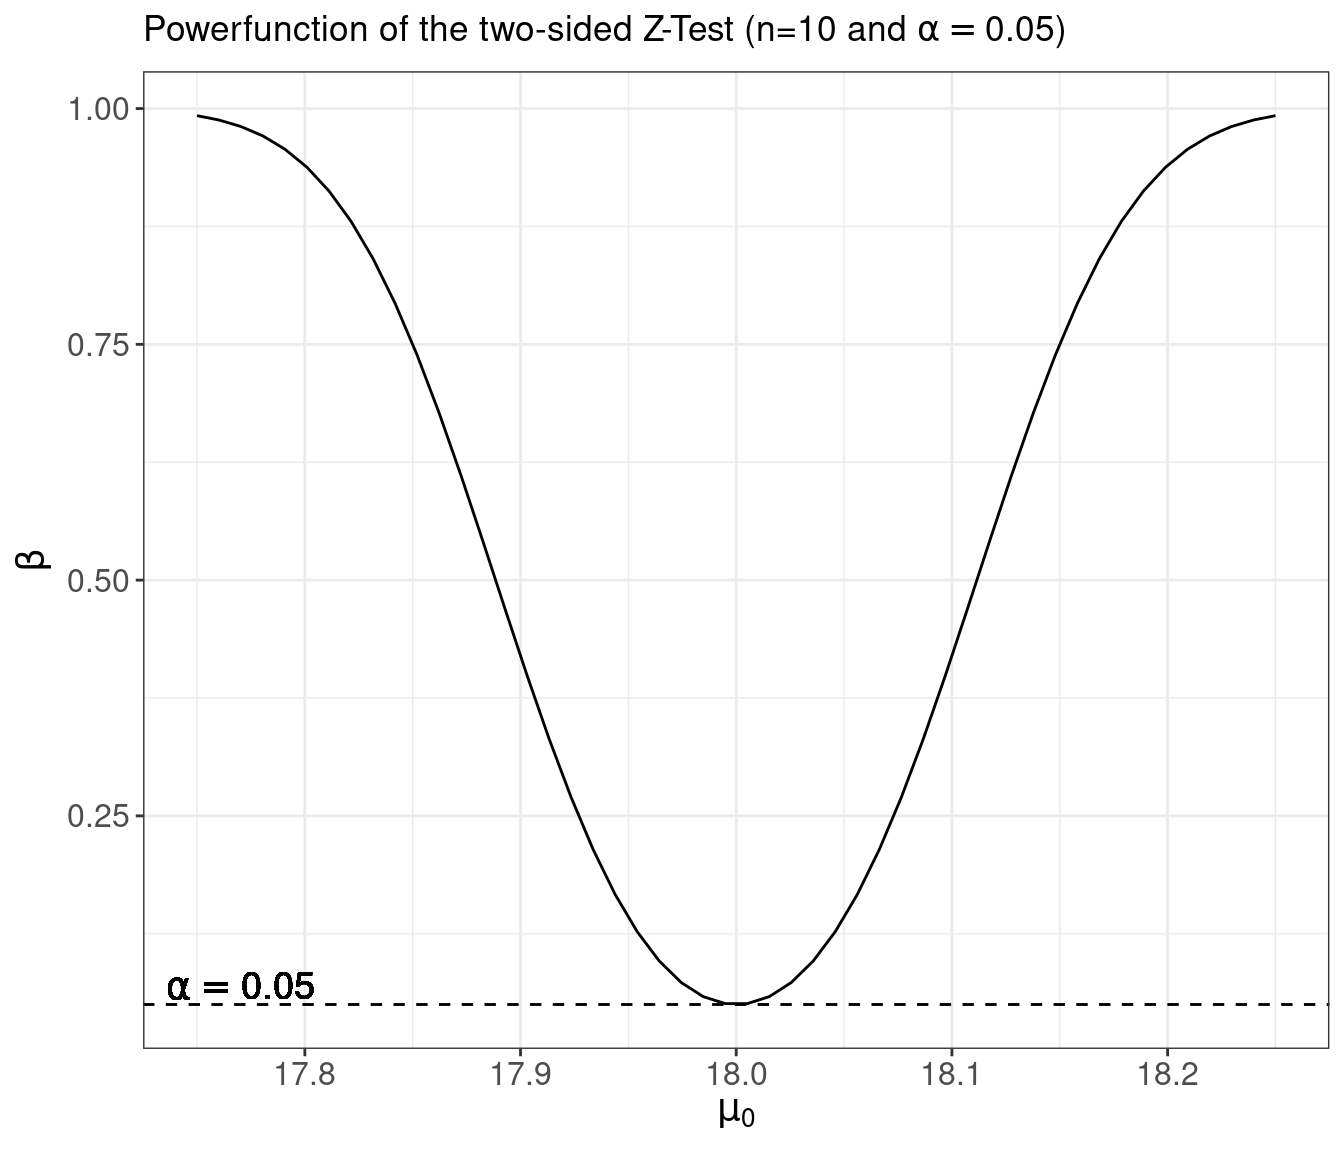
\includegraphics{03-Test-Theory_files/figure-latex/unnamed-chunk-4-1} \end{center}

This example illustrates the power function of a sensible test, since:

\begin{itemize}
\tightlist
\item
  Under \(H_0:\mu=\mu_0\) we have \(\beta_{n,\alpha}(\mu_0)=\alpha\).
\item
  The test is unbiased, since \(\beta_{n,\alpha}(\mu)\geq\alpha\) for any \(\mu\neq\mu_0\).
\item
  The test is consistent, since \(\lim_{n\rightarrow\infty} \beta_{n,\alpha}(\mu)=1\) for every fixed \(\mu\neq \mu_0\).
\item
  For fixed sample size \(n\), \(\beta_{n,\alpha}(\mu)\) increases as the distance \(|\mu-\mu_0|\) increases.
\item
  If \(|\mu-\mu_0|>|\mu^*-\mu_0|\) then \(\beta_{n,\alpha}(\mu)>\beta_{n,\alpha}(\mu^*)\).
\item
  \(\beta_{n,\alpha}(\mu)\) decreases as the significance level \(\alpha\) of the test decreases. I.e., if \(\alpha>\alpha^*\) then
  \(\beta_{n,\alpha}(\mu)>\beta_{n,\alpha^*}(\mu)\).
\end{itemize}

\hfill\break

Assuming that the basic assumptions (i.e., normality and known variance) are true, the above Gauss-test is the most prominent example of a \emph{uniformly most powerful} test. Under its (restrictive) assumptions, no other possible test can achieve a larger value of \(\beta_{n,\alpha}(\mu)\) for any possible value of \(\mu\).

\hypertarget{asymptotic-null-distributions}{%
\section{Asymptotic Null Distributions}\label{asymptotic-null-distributions}}

Generally, the underlying distributions are unknown. In this case it is usually not possible to compute the power function of a test for fixed \(n\). (Exceptions are so called ``distribution-free'' tests in nonparametric statistics.) The only way out of this difficulty is to rely on large sample asymptotics and corresponding asymptotic distributions, which allow to approximate the power function and to study the \textbf{asymptotic efficiency} of a test. The finite sample behavior of a test for different sample sizes \(n\) is then evaluated by means of \textbf{simulation studies}.

For a real-valued parameter \(\theta\) most tests of \(H_0:\theta=\theta_0\) rely on estimators \(\hat\theta\) of \(\theta\). Under suitable regularity conditions on the underlying distribution, central limit theorems usually imply that
\[\sqrt{n}(\hat\theta - \theta)\rightarrow_D N(0,v^2)\quad\text{as}\quad n\rightarrow\infty,\]
where \(v^2\) is the asymptotic variance of the estimator.

\hfill\break

Often a consistent estimator \(\hat v^2\) of \(v^2\) can be determined from the data. For large \(n\) we then approximately have
\[\frac{\sqrt{n}(\hat\theta - \theta)}{ v}\overset{a}{\sim} N(0,1).\]
For a given \(\alpha\), a one-sided test of \(H_0:\theta=\theta_0\) against \(H_1:\theta>\theta_0\) then rejects \(H_0\) if
\[
Z=\frac{\sqrt{n} (\hat\theta -\theta_0)}{v}>z_{1-\alpha}.
\]
The corresponding asymptotic approximation (valid for sufficiently large \(n\)) of the true power function is then given by
\[
\beta_{n,\alpha}(\theta) = 1-\Phi\left(z_{1-\alpha}-\frac{\sqrt{n} (\theta -\theta_0)}{v}\right)
\]

\hfill\break

Note that in practice the (unknown) true value \(v^2\) is generally replaced by an estimator \(\hat v^2\) determined from the data. As long as \(\hat v^2\) is a consistent estimator of \(v^2\) this leads to the same asymptotic power function. The resulting test is asymptotically unbiased and consistent.

\hfill\break

Usually there are many different possible estimators for a parameter \(\theta\). Consider an alternative estimator \(\tilde\theta\) of \(\theta\) satisfying
\[
\sqrt{n}(\tilde\theta - \theta)\rightarrow_D N(0,\tilde v^2) \quad\text{as}\quad n\rightarrow\infty.
\]
If the asymptotic variance \(v^2\) of the estimator \(\hat\theta\) is smaller than the asymptotic variance \(\tilde v^2\) of \(\tilde\theta\), i.e., \(v^2<\tilde v^2\), then \(\hat\theta\) is a \textbf{more efficient} estimator of \(\theta\). Then necessarily the test based on \(\hat\theta\) is \textbf{more powerful} than the test based on \(\tilde\theta\), since asymptotically for all \(\theta>\theta_0\)
\begin{align*}
\tilde\beta_{n,\alpha}(\theta) &= 1-\Phi\left(z_{1-\alpha}-\frac{\sqrt{n} (\theta -\theta_0)}{\tilde v}\right)\\
& < 1-\Phi\left(z_{1-\alpha}-\frac{\sqrt{n} (\theta -\theta_0)}{v}\right)=\beta_{n,\alpha}(\theta)
\end{align*}

\hfill\break

\textbf{Example:} Let \(X_1,\dots,X_n\) be an iid random sample. Consider testing \(H_0:\mu=\mu_0\) against \(H_1:\mu>\mu_0\), where \(\mu:=E(X_i)\). For a given level \(\alpha\) the t-test then rejects \(H_0\) if
\[
T=\frac{\sqrt{n}(\bar X-\mu_0)}{S}>t_{n-1;1-\alpha},
\]
where \(t_{n-1;1-\alpha}\) is the \(1-\alpha\) quantile of a t-distributions with \(n-1\)-degrees of freedom. This is an exact test if the distribution of \(X_i\) is normal. In the general case, the justification of the t-test is based on asymptotic arguments. Under some regularity conditions the central limit theorem implies that
\[
\sqrt{n}(\bar X - \mu)\rightarrow_D N(0,\sigma^2)\quad\text{as}\quad n\rightarrow\infty
\]
with \(\sigma^2=Var(X_i)\). Moreover, \(S^2\) is a consistent estimator of \(\sigma^2\) and \(t_{n-1;1-\alpha}\rightarrow z_{1-\alpha}\) as \(n\rightarrow \infty\). Thus even if the distribution of \(X_i\) is non-normal, for sufficiently large \(n\), \(T=\frac{\sqrt{n}(\bar X-\mu_0)}{S}\) is approximately \(N(0,1)\)-distributed and the asymptotic power function of the t-test is given by
\[
\beta_{n,\alpha}(\theta) = 1-\Phi\left(z_{1-\alpha}-\frac{\sqrt{n} (\mu -\mu_0)}{\sigma}\right).
\]

\hypertarget{multiple-comparisons}{%
\section{Multiple Comparisons}\label{multiple-comparisons}}

In statistics, the multiple comparisons, multiplicity or multiple testing problem occurs when one considers a set of statistical inferences simultaneously or infers a subset of parameters selected based on the observed values. Errors in inference, including confidence intervals that fail to include their corresponding population parameters or hypothesis tests that incorrectly reject the null hypothesis are more likely to occur when one considers the set as a whole.

In empirical studies often dozens or even hundreds of tests are performed for the same data set. When \textbf{searching} for
significant test results, one may come up with \textbf{false discoveries}.

\textbf{Example:} \(m\) different, independent test of significance level \(\alpha>0\). (Independence means that the test statistics used are mutually independent -- this is usually not true in practice). Let's assume that a common null hypothesis \(H_0\) holds for each of the \(m\) tests. Then

\[
P \begin{pmatrix}
      \text{Type I error}\\
      \text{by at least} \\
      \text{one of the $m$ tests}
  \end{pmatrix}
= 1 - (1 - \alpha)^m =: \alpha_m>\alpha
\]

Therefore, as \(m\) increases also the probability of a type I error increases:

\begin{longtable}[]{@{}ll@{}}
\toprule
Number of tests \(m\) & Probability of at least one type I error (\(\alpha_m\)) \\
\midrule
\endhead
1 & 0.050 \\
3 & 0.143 \\
5 & 0.226 \\
10 & 0.401 \\
100 & \textbf{0.994} \\
\bottomrule
\end{longtable}

\hfill\break

Analogous problem: Construction of \(m\) many \((1-\alpha)\) \textbf{confidence intervals}.
\[
P \begin{pmatrix}
      \text{at least one of the $m$ confidence} \\
      \text{intervals does not contain} \\
      \text{the true parameter value} \end{pmatrix}
    = 1 - (1-\alpha)^m>\alpha
\]

\hfill\break

\begin{figure}

{\centering \includegraphics{img/xkcd_mult_test} 

}

\caption{From: https://xkcd.com/882/}\label{fig:unnamed-chunk-5}
\end{figure}

This represents the general problem of multiple comparisons. In practice, it will not be true that all considered test statistics are mutually independent. (This even complicates the problem.) However, we will still have the effect that the probability of at least one falsely significant result increases with the number \(m\) of tests, but it will not be equal to \(1-(1-\alpha)^m\).

\hfill\break

A statistically rigorous \textbf{solution} of this problem consists in modifying the constructions of tests or confidence intervals in order to arrive at \textbf{simultaneous tests}:
\[
P\begin{pmatrix}
    \text{Type I error by} \\
    \text{at least one of the $m$ tests}
 \end{pmatrix} \leq \alpha
\]
or \textbf{simultaneous confidence intervals}:
\begin{align*}
&P \begin{pmatrix}
      \text{At least one of the $m$ confidence} \\
      \text{intervals does not contain} \\
      \text{the true parameter value}
  \end{pmatrix}  \leq \alpha\\[2ex]
\Leftrightarrow\quad 
&P \begin{pmatrix}
    \text{All confidence intervals} \\
    \text{simultaneously contain the} \\
    \text{true parameter values}
  \end{pmatrix} \geq 1 - \alpha
\end{align*}

\hfill\break

For certain problems (e.g., analysis of variance) there exist specific procedures for constructing
simultaneous confidence intervals. However, the only generally applicable procedure seems to be the
\textbf{Bonferroni correction}. It is based on Boole's inequality.

\textbf{Theorem (Boole):} Let \(A_1, A_2, \dots, A_m\) denote \(m\) different events. Then
\[
 P(A_1 \cup A_2 \cup \dots \cup A_m) \leq \sum_{i=1}^m P(A_i).
\]
This inequality also implies that:
\[
 P(A_1 \cap A_2 \cap \dots \cap A_m) \ge
  1 - \sum_{i=1}^m P(\bar A_i),
\]
where \(\bar A_i\) denotes the complementary event ``not \(A_i\)''.

\hfill\break

\textbf{Example: Bonferroni adjustment} for \(m\) different tests of level \(\alpha^* = \alpha/m\).
\[
P\begin{pmatrix}
\text{Type I error by} \\
\text{at least one of the $m$ tests}
\end{pmatrix}
\leq \sum_{i=1}^m \alpha^\ast = \alpha
\]

\hfill\break

Analogously: Construction of \(m\) many \((1-\alpha^*)\)-confidence intervals with \(\alpha^* =\alpha/m\):
\begin{align*}
&P\begin{pmatrix}
      \text{At least one of the $m$ confidence} \\
      \text{intervals does not contain} \\
      \text{the true parameter value} 
  \end{pmatrix}
\leq \sum_{i=1}^m \alpha^\ast = \alpha\\[2ex]
\Leftrightarrow\quad
&P\begin{pmatrix}
    \text{All confidence interval} \\
    \text{simultaneously contain the} \\
    \text{true parameter values}
  \end{pmatrix}
\geq 1 - \sum_{i=1}^m \alpha^\ast = 1 - \alpha
\end{align*}

\textbf{Example:}
Regression analysis with \(K=100\) regressors, where none of the variables has an effect on the dependent variable \(y\).

\begin{Shaded}
\begin{Highlighting}[]
\FunctionTok{library}\NormalTok{(}\StringTok{"tidyverse"}\NormalTok{, }\AttributeTok{quietly =} \ConstantTok{TRUE}\NormalTok{)}
\NormalTok{K }\OtherTok{\textless{}{-}} \DecValTok{100} \CommentTok{\# number of regressors}
\NormalTok{n }\OtherTok{\textless{}{-}} \DecValTok{500} \CommentTok{\# sample size}

\FunctionTok{set.seed}\NormalTok{(}\DecValTok{123}\NormalTok{)}

\CommentTok{\# Generate regression data, where none of the X{-}variables }
\CommentTok{\# has an effect on the dependent variable Y:}
\NormalTok{my\_df }\OtherTok{\textless{}{-}} \FunctionTok{matrix}\NormalTok{(}\AttributeTok{data =} \FunctionTok{rnorm}\NormalTok{(}\AttributeTok{n =}\NormalTok{ n}\SpecialCharTok{*}\NormalTok{K), }
                \AttributeTok{nrow =}\NormalTok{ n, }\AttributeTok{ncol =}\NormalTok{ K, }
                \AttributeTok{dimnames =} \FunctionTok{list}\NormalTok{(}\FunctionTok{paste0}\NormalTok{(}\StringTok{"i."}\NormalTok{,}\DecValTok{1}\SpecialCharTok{:}\NormalTok{n), }
                                \FunctionTok{paste0}\NormalTok{(}\StringTok{"X."}\NormalTok{,}\DecValTok{1}\SpecialCharTok{:}\NormalTok{K))) }\SpecialCharTok{\%\textgreater{}\%} 
  \FunctionTok{as\_tibble}\NormalTok{() }\SpecialCharTok{\%\textgreater{}\%} 
  \FunctionTok{mutate}\NormalTok{(}\AttributeTok{Y =} \FunctionTok{rnorm}\NormalTok{(n)) }\SpecialCharTok{\%\textgreater{}\%} \CommentTok{\# Adding a Y{-}variable that is independent of the X{-}variables}
  \FunctionTok{select}\NormalTok{(Y, }\FunctionTok{everything}\NormalTok{())  }

\CommentTok{\# OLS regression}
\NormalTok{OLS\_result\_df }\OtherTok{\textless{}{-}} \FunctionTok{lm}\NormalTok{(Y }\SpecialCharTok{\textasciitilde{}}\NormalTok{ . , }\AttributeTok{data =}\NormalTok{ my\_df) }\SpecialCharTok{\%\textgreater{}\%} 
\NormalTok{  summary }\SpecialCharTok{\%\textgreater{}\%} 
\NormalTok{  broom}\SpecialCharTok{::}\FunctionTok{tidy}\NormalTok{()}


\NormalTok{Count\_Signif }\OtherTok{\textless{}{-}}\NormalTok{ OLS\_result\_df }\SpecialCharTok{\%\textgreater{}\%} 
  \FunctionTok{filter}\NormalTok{(term }\SpecialCharTok{!=} \StringTok{\textquotesingle{}(Intercept)\textquotesingle{}}\NormalTok{) }\SpecialCharTok{\%\textgreater{}\%} 
  \FunctionTok{count}\NormalTok{(p.value }\SpecialCharTok{\textless{}} \FloatTok{0.05}\NormalTok{)}
\end{Highlighting}
\end{Shaded}

\begin{verbatim}
## # A tibble: 2 x 2
##   `p.value < 0.05`     n
## * <lgl>            <int>
## 1 FALSE               96
## 2 TRUE                 4
\end{verbatim}

\hypertarget{r-lab-the-gauss-test}{%
\section{R-Lab: The Gauss-Test}\label{r-lab-the-gauss-test}}

Let's reconsider the simplest test statistic you will ever meet: The \textbf{Gauss-Test} (Or ``Z-Test'').

\textbf{Setup:} Let \(X_1,\dots,X_n\) be an iid random sample with \(X_i\sim N(\mu,\sigma^2)\) and \(\sigma^2<\infty.\)

\textbf{Idea:} Under the above setup, \(\bar{X}_n=n^{-1}\sum_{i=1}^n X_i\) consistently estimates the (unknown) true mean value \(\mu\). That is, \(\bar{X}_n\to_p\mu\).

\begin{itemize}
\tightlist
\item
  Under the null hypothesis (i.e., \(\mu_{0}=\mu\)), the difference \(\bar{X}_n-\mu_{0}\) should be ``small''.
\item
  Under the alternative hypothesis (i.e., \(\mu_{0}\neq\mu\)), the difference \(\bar{X}_n-\mu_{0}\) should be ``large''.
\end{itemize}

\hfill\break

Under the null hypothesis \(H_0\) we have that \(\mu_{0}=\mu\). Therefore:
\[
Z=\frac{\sqrt{n}\,(\bar{X}_n-\mu_{0})}{\sigma}=\underbrace{\frac{\sqrt{n}\,(\bar{X}_n-\mu)}{\sigma}}_{\sim N(0,1)}
\]

\hfill\break

Under the alternative \(H_1\) we have that \(\;\mu_{0}\neq \mu\). Therefore:
\begin{align*}
Z&=\frac{\sqrt{n}\,(\bar{X}_n-\mu_{0})}{\sigma}\\
&=\frac{\sqrt{n}\,(\bar{X}_n-\mu_{0}+\mu-\mu)}{\sigma}\\
&=\frac{\sqrt{n}\,(\bar{X}_n-\mu)}{\sigma}+{\color{blue}{ \frac{\sqrt{n}\,(\mu-\mu_{0})}{\sigma} }} \sim N\left({\color{blue}{\frac{\sqrt{n}\,(\mu-\mu_{0})}{\sigma}}},1\right)
\end{align*}

The different distributions (under \(H_0\) and \(H_1\)) of the test statistic \(Z\) can be investigated in the following dynamic plot:

\begin{figure}

{\centering \includegraphics{img/Gauss-Test-Distr} 

}

\caption{See: https://dliebl.shinyapps.io/Gauss-Test-Distr/}\label{fig:unnamed-chunk-10}
\end{figure}

\hypertarget{ordinary-least-squares-the-classical-linear-regression-model}{%
\chapter{Ordinary Least Squares: The Classical Linear Regression Model}\label{ordinary-least-squares-the-classical-linear-regression-model}}

\hypertarget{finite-sample-properties}{%
\section{Finite-Sample Properties}\label{finite-sample-properties}}

\textbf{Notation:}

\begin{itemize}
\item
  \(y_i \,\) dependent variable.
\item
  \(x_{ik} \,\) \(k\)th independent variable (or regressor) with
  \(k=1,\dots,K \,\).\\
  Can be stochastic or deterministic.
\item
  \(\varepsilon_i \,\) stochastic error term
\item
  \(i \,\) indexes the \(i\)th individual with \(i=1,\dots,n\), where \(n\) is
  the sample size
\end{itemize}

\textbf{Assumption 1.1: Linearity}

\begin{align}
y_i = \sum_{k=1}^K\beta_k x_{ik}+\varepsilon_i, \quad i=1,\dots,n \,.
\label{eq:c3e1}
\end{align}

Usually, a constant (or intercept) is included, in this case \(x_{i1}=1\) for all \(i\). In the following we will always assume that a constant is included in the linear model, unless otherwise stated. A special case of the above defined linear model is the so-called \emph{simple linear model}, defined as

\begin{align*}
y_i = \beta_1+\beta_2 x_i +\varepsilon_i, \quad i=1,\dots,n \,.
\end{align*}

Often it is convenient to write \eqref{eq:c3e1} using matrix notation

\begin{align}
y_i = \mathbf{x}_i'\boldsymbol{\beta} +\varepsilon_i, \quad i=1,\dots,n \,,
\label{eq:c3e3}
\end{align}

where \(\mathbf{x}_i=(x_{i1},\dots,x_{iK})'\) and \(\boldsymbol{\beta}=(\beta_1,\dots,\beta_K)'\). Stacking all individual rows \(i\) leads to

\begin{align*}
\underset{(n\times 1)}{\mathbf{y}} = \underset{(n\times K)}{\mathbf{X}}\underset{(K\times 1)}{\boldsymbol{\beta}} + \underset{(n\times 1)}{\boldsymbol{\varepsilon}} \, ,
\end{align*}

where

\begin{align*}
\mathbf{y} = \left(\begin{matrix}y_1\\ \vdots\\y_n\end{matrix}\right),\quad
\mathbf{X} = \left( \begin{matrix}
x_{11} & \dots & x_{1K} \\ \vdots & \ddots & \vdots \\ x_{n1} &\dots&x_{nK}\\
\end{matrix}\right),\quad\text{and}\quad \boldsymbol{\varepsilon}=\left(\begin{matrix}\varepsilon_1\\ \vdots\\ \varepsilon_n\end{matrix}\right).
\end{align*}

We begin our analysis of the model in Eq. \eqref{eq:c3e3} under the framework of the so-called \emph{classic assumptions}.

\hfill\break

\textbf{Assumption 1.2: Strict Exogeneity}

\[\mathbb{E}(\varepsilon_i|\mathbf{X}) = 0\]

or equivalently stated for the vector \(\boldsymbol{\varepsilon}\)

\[\mathbb{E}(\boldsymbol{\varepsilon}|\mathbf{X}) = \mathbf{0}.\]

Notice that in the presence of a constant regressor, setting the expectation to zero is a normalization. Note that in econometrics, where we typically have to work with quasi-experimental data, strict exogeneity is a very strong assumption. It also cannot be fulfilled when the regressors include lagged dependent variables.

\textbf{Some Implications of Strict Exogeneity:}

\begin{itemize}
\tightlist
\item
  The unconditional mean of the error term is zero:
\end{itemize}

\begin{align}
\mathbb{E}(\varepsilon_i) = 0\quad(i=1,\dots,n)
\label{eq:c3e4}
\end{align}

\textbf{Proof}
From the \emph{Law of Total Expectations} (i.e., \(\mathbb{E}(\mathbb{E}(y|\mathbf{x}))=\mathbb{E}(y)\)) it follows that
\begin{align*}
\mathbb{E}(\varepsilon_i)=\mathbb{E}(\mathbb{E}(\varepsilon_i|\mathbf{X})).
\end{align*}
The strict exogeneity assumption then yields
\begin{align*}
\mathbb{E}(\mathbb{E}(\varepsilon_i|\mathbf{X}))=\mathbb{E}(0)=0.
\end{align*}
qed.

\hfill\break

\begin{itemize}
\tightlist
\item
  Generally, two random variables \(x\) and \(y\) are said to be
  \textbf{orthogonal} if their cross moment is zero: \(\mathbb{E}(xy)=0\). Under
  strict exogeneity, the regressors are orthogonal to the error term
  for \emph{all} observations, i.e.,
  \begin{align}
   \mathbb{E}(x_{jk}\varepsilon_i) = 0\quad(i,j=1,\dots,n; k=1,\dots,K)
   \label{eq:c3e5}
   \end{align}
\end{itemize}

\textbf{Proof}
\begin{align*}
      \mathbb{E}(x_{jk}\varepsilon_i) &= \mathbb{E}(\mathbb{E}(x_{jk}\varepsilon_i|x_{jk}))\quad{\text{(Law of Total Expect.)}}\\
       &= \mathbb{E}(x_{jk}\mathbb{E}(\varepsilon_i|x_{jk}))\;\;{\text{(Linearity of $\mathbb{E}$-operator)}}
\end{align*}

Now, to show that \(\mathbb{E}(x_{jk}\varepsilon_i)=0\), we need to show that \(\mathbb{E}(\varepsilon_i|x_{jk})=0\), which is done in the following:
Since \(x_{jk}\) is an element of \(\mathbf{X}\), the \emph{Law of Iterated Expectations} (i.e., \(\mathbb{E}(\mathbb{E}(y|\mathbf{x},\mathbf{z})|\mathbf{x})=\mathbb{E}(y|\mathbf{x})\))
implies that \[\mathbb{E}(\mathbb{E}(\varepsilon_i|\mathbf{X})|x_{jk})=\mathbb{E}(\varepsilon_i|x_{jk}).\] The
strict exogeneity assumption yields
\[\mathbb{E}(\mathbb{E}(\varepsilon_i|\mathbf{X})|x_{jk})=\mathbb{E}(0|x_{jk})=0.\] I.e., we have that
\[\mathbb{E}(\varepsilon_i|x_{jk})=0,\] which allows us to conclude that
\[\mathbb{E}(x_{jk}\varepsilon_i)=\mathbb{E}(x_{jk}\mathbb{E}(\varepsilon_i|x_{jk}))=\mathbb{E}(x_{jk}0)=0.\]
qed

\hfill\break

\begin{itemize}
\tightlist
\item
  Because the mean of the error term is zero (\(\mathbb{E}(\varepsilon_i)=0\) for all
  \(i\)), it follows that the orthogonality property
  (\(\mathbb{E}(x_{jk}\varepsilon_i)=0\), for all \(i,j,k\)) is equivalent to a
  zero-correlation property. I.e., that
  \begin{align}
    Cov(\varepsilon_i,x_{jk}) = 0;\; i,j=1,\dots,n; k=1,\dots,K
     \label{eq:c3e6}
  \end{align}
  Therefore, the strict exogeneity assumption implies the requirement
  that regressors are uncorrelated with the current (\(i=j\)), the past
  (\(i<j\)) and the future (\(i>j\)) error terms. Of course, this is
  usually found to be a too strong assumption - particularly in
  time-series contexts.
\end{itemize}

\textbf{Proof}
\begin{align*}
      Cov(\varepsilon_i,x_{jk}) &= \mathbb{E}(x_{jk}\varepsilon_i)-\mathbb{E}(x_{jk})\,\mathbb{E}(\varepsilon_i)\quad{\text{(Def.~of Cov)}}\\
       &= \mathbb{E}(x_{jk}\varepsilon_i)\\
       &= 0
\end{align*}

Where the second equal sign holds since \(\mathbb{E}(\varepsilon_i)=0\) (see Eq. \eqref{eq:c3e4}) and the third because of orthogonality (see Eq. \eqref{eq:c3e5}).
qed

\hfill\break

\textbf{Assumption 1.3: Rank Condition}

\[rank(\mathbf{X})=K\quad\text{a.s.}\]

This assumption demands that the event of one regressor being linearly
dependent on the others occurs with a probability equal to zero. (This
is the literal translation of the "almost surely (a.s.)" concept.)
This assumption also implies the assumption that \(n\geq K\).\\
This assumption is a bit dicey and its violation belongs to one of the
classic problems in applied econometrics (keywords: multicollinearity,
dummy variable trap, variance inflation). The violation of this
assumption harms any economic interpretation as we cannot disentangle
the regressors' individual effects on \(\mathbf{y}\). Therefore, this
assumption is often referred to as an \emph{identification} assumption.\\

\textbf{Assumption 1.4: Spherical Error}

\begin{align*}
\mathbb{E}(\varepsilon_i^2|\mathbf{X}) &= \sigma^2>0\\
\mathbb{E}(\varepsilon_i\varepsilon_j|\mathbf{X}) &= 0,\quad\quad i\neq j.
\end{align*}

Or more compactly written as,

\begin{align*}
\mathbb{E}(\boldsymbol{\varepsilon}\boldsymbol{\varepsilon}'|\mathbf{X}) = \sigma^2 I_n,\quad\quad \sigma^2>0.
\end{align*}

Thus, we assume that, for a given realization of \(\mathbf{X}\), the error
process is uncorrelated (\(\mathbb{E}(\varepsilon_i\varepsilon_j|\mathbf{X})=0\), for all
\(i\neq j\)) and homoscedastic (same \(\sigma^2\), for all \(i\)).

\hypertarget{the-algebra-of-least-squares}{%
\subsection{The Algebra of Least Squares}\label{the-algebra-of-least-squares}}

The OLS estimator \(\mathbf{b}\) is defined as the minimizer of a specific loss
function termed \emph{the sum of squared residuals}

\begin{align*}
SSR(\mathbf{b}^\ast) = \sum_{i=1}^n(y_i-\mathbf{x}_i'\mathbf{b}^\ast)^2\;=\;(\mathbf{y}-\mathbf{X}\mathbf{b}^\ast)'(\mathbf{y}-\mathbf{X}\mathbf{b}^\ast).
\end{align*}

I.e., we have

\begin{align*}
  \mathbf{b}&:=\arg\min_{\mathbf{b}^\ast\in\mathbb{R}^K}SSR(\mathbf{b}^\ast),
\end{align*}
We can easily minimize \(SSR(\mathbf{b}^\ast)\) in closed form:

\begin{align*}
SSR(\mathbf{b}^\ast)
&= (\mathbf{y}-\mathbf{X}\mathbf{b}^\ast)'(\mathbf{y}-\mathbf{X}\mathbf{b}^\ast)\\
 &= \mathbf{y}'\mathbf{y}-(\mathbf{X}\mathbf{b}^{\ast})'\mathbf{y}-\mathbf{y}'\mathbf{X}\mathbf{b}^{\ast}+\mathbf{b}^{\ast'}\mathbf{X}'\mathbf{X}\mathbf{b}^{\ast}\\
    &= \mathbf{y}'\mathbf{y}-2\mathbf{y}'\mathbf{X}\mathbf{b}^{\ast}+\mathbf{b}^{\ast'}\mathbf{X}'\mathbf{X}\mathbf{b}^{\ast}\\[2ex]
   \Rightarrow\quad\frac{d}{d\mathbf{b}^{\ast}}SSR(\mathbf{b}^{\ast}) &= -2\mathbf{X}'\mathbf{y}+2\mathbf{X}'\mathbf{X}\mathbf{b}^{\ast}
\end{align*}

Setting the first derivative so zero yields the so-called \emph{normal
equations}

\begin{align*}
\mathbf{X}'\mathbf{X}\mathbf{b} = \mathbf{X}'\mathbf{y},
\end{align*}

which lead to the OLS estimator

\begin{align}
\mathbf{b} = (\mathbf{X}'\mathbf{X})^{-1}\mathbf{X}'\mathbf{y},
\label{eq:c3e7}
\end{align}

where \((\mathbf{X}'\mathbf{X})^{-1}\) exists (a.s.) because of our full
rank assumption (Assumption 3).\\
Often it is useful to express \(\mathbf{b}\) (and similar other
estimators) in sample moment notation:

\[\mathbf{b}=\mathbf{S}_{\mathbf{x}\mathbf{x}}^{-1}\mathbf{s}_{\mathbf{x}\mathbf{y}},\]

where
\(\mathbf{S}_{\mathbf{x}\mathbf{x}}=n^{-1}\mathbf{X}'\mathbf{X}=n^{-1}\sum_i\mathbf{x}_i\mathbf{x}_i'\)
and
\(\mathbf{s}_{\mathbf{x}\mathbf{y}}=n^{-1}\mathbf{X}'\mathbf{y}=n^{-1}\sum_i\mathbf{x}_iy_i\).
This notation is more convenient for developing our large sample
results.\\

\hypertarget{some-quantities-of-interest}{%
\subsection*{Some quantities of interest:}\label{some-quantities-of-interest}}
\addcontentsline{toc}{subsection}{Some quantities of interest:}

\begin{itemize}
\item
  The \emph{(OLS) fitted value}: \(\hat{y}_i=\mathbf{x}_i\mathbf{b}\)\\
  In matrix notation:
  \(\hat{\mathbf{y}}=\mathbf{X}(\mathbf{X}'\mathbf{X})^{-1}\mathbf{X}'\mathbf{y} = \mathbf{P}\mathbf{y}\)
\item
  The \emph{(OLS) residual}: \(\hat{\varepsilon_i}=y_i-\hat{y}_i\)\\
  In matrix notation:
  \(\hat{\boldsymbol{\varepsilon}} = \mathbf{y}-\hat{\mathbf{y}} = \left(\mathbf{I}_n-\mathbf{X}(\mathbf{X}'\mathbf{X})^{-1}\mathbf{X}'\right)\mathbf{y} = \mathbf{M}\mathbf{y}\),
\end{itemize}

where \(\mathbf{P}=\mathbf{X}(\mathbf{X}'\mathbf{X})^{-1}\mathbf{X}'\) is
a so-called orthogonal projection matrix that projects any vector into
the column space spanned by \(\mathbf{X}\) and
\(\mathbf{M}=\mathbf{I}_n-\mathbf{X}(\mathbf{X}'\mathbf{X})^{-1}\mathbf{X}'\)
is the associated orthogonal projection matrix that projects any vector
into the vector space that is orthogonal to that spanned by
\(\mathbf{X}\). Projection matrices have some nice properties, listed in
the following lemma.

\textbf{Lemma 3.1.1 (Orthogonal Projection matrices)}
For \(\mathbf{P}=\mathbf{X}(\mathbf{X}'\mathbf{X})^{-1}\mathbf{X}'\) and
\(\mathbf{M}=\mathbf{I}_n-\mathbf{P}\) with \(\mathbf{X}\) being of full
rank it holds:

\begin{itemize}
\item
  \(\mathbf{P}\) and \(\mathbf{M}\) are symmetric and idempotent, i.e.:
  \[\mathbf{P}\mathbf{P}=\mathbf{P}\quad\text{ and }\quad \mathbf{M}\mathbf{M}=\mathbf{M}.\]
\item
  Further properties:
  \[\mathbf{X}'\mathbf{P}=\mathbf{X}',\quad \mathbf{X}'\mathbf{M}=\mathbf{0},\quad\text{ and }\quad \mathbf{P}\mathbf{M}=\mathbf{0}.\]
\end{itemize}

Proofs follow directly from the definitions of \(\mathbf{P}\) and
\(\mathbf{M}\).\\
Using these results we obtain the following proposition on the OLS
residuals and OLS fitted values.

\textbf{Proposition 3.1.2 (OLS residuals)}
For the OLS residuals and the OLS fitted values it holds that

\begin{align*}
    \mathbf{X}'\hat{\boldsymbol{\varepsilon}} &= \mathbf{0}, \quad\text{and}\\
    \mathbf{y}'\mathbf{y} &= \hat{\mathbf{y}}'\hat{\mathbf{y}}+\hat{\boldsymbol{\varepsilon}}'\hat{\boldsymbol{\varepsilon}}.
\end{align*}

\textbf{Proof}
The first result can be shown as following:
\begin{align*}
  \mathbf{X}'\hat{\boldsymbol{\varepsilon}}
   &= \mathbf{X}'\mathbf{M}\mathbf{y}\quad\text{(By Def. of $\mathbf{M}$)}\\
   &= \mathbf{0}\mathbf{y}\quad\text{(By Lemma 3.1.1 part (ii))}\\
   &= \underset{(K\times 1)}{\mathbf{0}}
\end{align*}

The second result follows from:
\begin{align*}
  \mathbf{y}'\mathbf{y} &= (\mathbf{P}\mathbf{y}+\mathbf{M}\mathbf{y})'(\mathbf{P}\mathbf{y}+\mathbf{M}\mathbf{y})\quad\text{(By Def.~of $\mathbf{P}$ and $\mathbf{M}$)}\\
   &= (\mathbf{y}'\mathbf{P}'+\mathbf{y}'\mathbf{M}')(\mathbf{P}\mathbf{y}+\mathbf{M}\mathbf{y})\\
   &= \mathbf{y}'\mathbf{P}'\mathbf{P}\mathbf{y}+\mathbf{y}'\mathbf{M}'\mathbf{M}\mathbf{y}+\mathbf{0}\quad\text{(By Lemma 3.1.1 part (ii))}\\
   &= \hat{\mathbf{y}}'\hat{\mathbf{y}}+\hat{\boldsymbol{\varepsilon}}'\hat{\boldsymbol{\varepsilon}}
\end{align*}
qed

\hfill\break

The vector of residuals \(\hat{\boldsymbol{\varepsilon}}\) has only \(n-K\) so-called \emph{degrees of freedom}. The vector looses \(K\) degrees of freedom, since it has to
satisfy the \(K\) linear restrictions (\(\mathbf{X}'\hat{\boldsymbol{\varepsilon}}=\mathbf{0}\)).
Particularly, in the case with intercept we have that
\(\sum_{i=1}^n\hat{\boldsymbol{\varepsilon}_i}=\mathbf{0}\).\\
This loss of \(K\) degrees of freedom also appears in the definition of
the \emph{unbiased} variance estimator

\begin{align}
s^2 = \frac{1}{n-K}\sum_{i=1}^n\hat{\varepsilon_i^2}.
\label{eq:c3e8}
\end{align}

\hypertarget{coefficient-of-determination}{%
\subsection{Coefficient of determination}\label{coefficient-of-determination}}

The total sample variance of the dependent variable
\(\sum_{i=1}^n\left(y_i-\bar{y}\right)^2\), where
\(\bar{y}=\frac{1}{n}\sum_{i=1}^ny_i\), can be decomposed as following:

\textbf{Proposition 3.1.3 (Variance decomposition)}
For the OLS regression of the linear model (\eqref{eq:c3e1} with intercept it holds that
\begin{align*}
  \underset{\text{total variance}}{\sum_{i=1}^n\left(y_i-\bar{y}\right)^2} = \underset{\text{explained variance}}{\sum_{i=1}^n\left(\hat{y}_i-\bar{\hat{y}}\right)^2}+\underset{\text{unexplained variance}}{\sum_{i=1}^n\hat{\varepsilon_i^2 \,\,.}}
\end{align*}

\textbf{Proof}

\begin{itemize}
\item
  As a consequence of Prop. 3.1.2 we have for regressions with intercept:
  \(\sum_{i=1}^n\hat{\varepsilon_i=0}\). Hence, from \(y_i=\hat{y}_i+\hat{\varepsilon_i}\)
  it follows that
  \begin{align*}
      \frac{1}{n}\sum_{i=1}^n y_i &= \frac{1}{n}\sum_{i=1}^n \hat{y}_i+\frac{1}{n}\sum_{i=1}^n \hat{\varepsilon_i} \\
      \bar{y} &= \bar{\hat{y}}_i+0
    \end{align*}
\item
  From Prop. 3.1.2 we know that:
  \begin{align*}
  \mathbf{y}'\mathbf{y} &= \hat{\mathbf{y}}'\hat{\mathbf{y}}+\hat{\boldsymbol{\varepsilon}}'\hat{\boldsymbol{\varepsilon}} \\
       \mathbf{y}'\mathbf{y} -n\bar{y}^2 &= \hat{\mathbf{y}}'\hat{\mathbf{y}}-n\bar{y}^2+\hat{\boldsymbol{\varepsilon}}'\hat{\boldsymbol{\varepsilon}} \\
       \mathbf{y}'\mathbf{y}-n\bar{y}^2 &= \hat{\mathbf{y}}'\hat{\mathbf{y}}-n\bar{\hat{y}}^2+\hat{\boldsymbol{\varepsilon}}'
       \hat{\boldsymbol{\varepsilon}}\quad\text{(By our result above.)} \\
       \sum_{i=1}^n y_i^2-n\bar{y}^2 &= \sum_{i=1}^n\hat{y}_i^2-n\bar{\hat{y}}^2+\sum_{i=1}^n\hat{\varepsilon}_i^2 \\
       \sum_{i=1}^n (y_i-\bar{y})^2 &= \sum_{i=1}^n (\hat{y}_i-\bar{\hat{y}})^2+\sum_{i=1}^n \hat{\varepsilon}_i^2
  \end{align*}
  qed
\end{itemize}

\hfill\break

The larger the proportion of the explained variance, the better is the
fit of the model. This motivates the definition of the so-called \(R^2\)
coefficient of determination:
\begin{align*}
  R^2=\frac{\sum_{i=1}^n\left(\hat{y}_i-\bar{\hat{y}}\right)^2}{\sum_{i=1}^n\left(y_i-\bar{y}\right)^2}\;=\;1-\frac{\sum_{i=1}^n\hat{u}_i^2}{\sum_{i=1}^n\left(y_i-\bar{y}\right)^2}
\end{align*}

Obviously, we have that \(0\leq R^2\leq 1\). The closer \(R^2\) lies to \(1\),
the better is the fit of the model to the observed data. However, a
high/low \(R^2\) does not mean a validation/falsification of the estimated
model. Any relation (i.e., model assumption) needs a plausible
explanation from relevant economic theory.

The most often criticized disadvantage of the \(R^2\) is that additional
regressors (relevant or not) will always increase the \(R^2\).

\textbf{Proposition 3.1.4 (\(R^2\) increase)}

Let \(R^2_1\) and \(R^2_2\) result from
\begin{align*}
    \mathbf{y} &= \mathbf{X}_1\mathbf{b}_{11}+\hat{\boldsymbol{\varepsilon}_1} \quad\text{and}\\
    \mathbf{y} &= \mathbf{X}_1\mathbf{b}_{21}+\mathbf{X}_2\mathbf{b}_{22}+\hat{\boldsymbol{\varepsilon}_2}.
\end{align*}

It then holds that \(R^2_2\geq R^2_1\).

\textbf{Proof}
Consider the sum of squared residuals,

\begin{align*}
S(\mathbf{\mathfrak{b}}_{21},\mathbf{\mathfrak{b}}_{22})=(\mathbf{y}-\mathbf{X}_1\mathbf{\mathfrak{b}}_{21}+\mathbf{X}_2\mathbf{\mathfrak{b}}_{22})'(\mathbf{y}-\mathbf{X}_1\mathbf{\mathfrak{b}}_{21}+\mathbf{X}_2\mathbf{\mathfrak{b}}_{22})
\end{align*}
By definition, this sum is minimized by the OLS estimators \(\mathbf{b}_{21}\)
and \(\mathbf{b}_{22}\), i.e.,
\(S(\mathbf{b}_{21},\mathbf{b}_{22})\leq S(\mathbf{\mathfrak{b}}_{21},\mathbf{\mathfrak{b}}_{22})\).
Consequently,
\begin{align*}
\hat{\boldsymbol{\varepsilon}}_{2}'\hat{\boldsymbol{\varepsilon}}_{2}=S(\mathbf{b}_{21},\mathbf{b}_{22})\leq S(\mathbf{b}_{11},0)=\hat{\boldsymbol{\varepsilon}}_{1}'\hat{\boldsymbol{\varepsilon}}_{1}
\end{align*}
which implies the statement:
\begin{align*}
R_2^2=1-\frac{\hat{\boldsymbol{\varepsilon}}_{2}'\hat{\boldsymbol{\varepsilon}}_{2}}{\sum_{i=1}^n\left(y_i-\bar{y}\right)^2}\geq
1-\frac{\hat{\boldsymbol{\varepsilon}}_{1}'\hat{\boldsymbol{\varepsilon}}_{1}}{\sum_{i=1}^n\left(y_i-\bar{y}\right)^2}=R_1^2
\end{align*}
qed

\hfill\break

Because of this, the \(R^2\) cannot be used as a criterion for model selection. Possible solutions are given by penalized criterions such as the so-called \emph{adjusted \(R^2\)} defined as

\begin{align*}
  \overline{R}^2 &= 1-\frac{ \frac{1}{n-K} \sum_{i=1}^n \hat{u}_i^2}{ \frac{1}{n-1} \sum_{i=1}^n \left(y_i-\bar{y}\right)^2} \\
   &= 1-\frac{n-1}{n-K}\left(1-R^2\right) \\
    &= 1-\frac{n-1}{n-K}+\frac{n-1}{n-K}R^2\quad+\frac{K-1}{n-K}R^2-\frac{K-1}{n-K}R^2 \\
    &= 1-\frac{n-1}{n-K}+R^2\quad+\frac{K-1}{n-K}R^2 \\
    &= -\frac{K-1}{n-K}+R^2\quad+\frac{K-1}{n-K}R^2 \\
   &= R^2-\frac{K-1}{n-K}\left(1-R^2\right) \leq R^2
\end{align*}

The adjustment is in terms of degrees of freedom.

\hypertarget{partitioned-regression-model}{%
\subsection*{Partitioned regression model}\label{partitioned-regression-model}}
\addcontentsline{toc}{subsection}{Partitioned regression model}

Already in the first edition of Econometrica (1933) Frisch and Waugh
pointed to an interesting property of multivariate linear regression
analysis, which was later generalized to by Lovell (1963). The so-called
Frisch-Waugh-Lovell (FWL) theorem points to a property of the OLS
estimation method, which allows to gain a deeper understanding of the
estimation method that is useful for the interpretation of the estimated
coefficients.

\begin{align}
  \mathbf{y} &= \mathbf{X}_1\mathbf{b}_1+\mathbf{X}_2\mathbf{b}_2+\hat{\boldsymbol{\varepsilon}} =  (\mathbf{X}_1,\mathbf{X}_2)\left(\begin{matrix}\mathbf{b}_1\\\mathbf{b}_2\end{matrix}\right)+\hat{\boldsymbol{\varepsilon}},
\label{eq:c3e9}
\end{align}

where \(rank(\mathbf{X}_j)=K_j\) for \(j=1,2\).\\
A regression of \(\mathbf{y}\) only on \(\mathbf{X}_2\) (not on \(\mathbf{X}_1\)), which
however \emph{takes into account the effect of \(\mathbf{X}_1\)}, has to be done as
following:
\begin{align}
  \mathbf{M}_1\mathbf{y} = \mathbf{M}_1\mathbf{X}_2\hat{\boldsymbol{\beta}}_2+\hat{\mathbf{v}},
\label{eq:c3e10}
\end{align}
where \(\mathbf{M}_1=\mathbf{I}_n-\mathbf{X}_1(\mathbf{X}_1'\mathbf{X}_1)^{-1}\mathbf{X}_1'\). Note that (\eqref{eq:c3e10} is a regression model full of residuals: The dependent variables \(\mathbf{M}_1\mathbf{y}\) are the residuals from regressing \(\mathbf{y}\) on \(\mathbf{X}_1\) and the \(K_2\) columns in the matrix of independent variables \(\mathbf{M}_1\mathbf{X}_2\) are the residuals from the regressing \(\mathbf{X}_2\) column-wise on \(\mathbf{X}_1\). This means that the variables \(\mathbf{M}_1\mathbf{y}\) and \(\mathbf{M}_1\mathbf{X}_2\) contain only those parts of \(\mathbf{y}\) and \(\mathbf{X}_2\), which are orthogonal to \(\mathbf{X}_1\); the effect of \(\mathbf{X}_1\) is ``\emph{partialled out}''. By the FWL theorem we have that:

\textbf{Proposition 3.1.5 (Frisch-Waugh-Lovell theorem)}
For the equations (\eqref{eq:c3e9}) and \eqref{eq:c3e10}) it holds that:
\[\hat{\boldsymbol{\beta}}_2=\mathbf{b}_2\quad\text{and}\quad \hat{\boldsymbol{\varepsilon}}=\hat{\mathbf{v}}.\]

\textbf{Proof}
The OLS estimator \(\hat{\boldsymbol{\beta}}_2\) is given by
\begin{align}
\hat{\boldsymbol{\beta}}_2 &= \left((\mathbf{M}_1\mathbf{X}_2)'(\mathbf{M}_1\mathbf{X}_2)\right)^{-1}(\mathbf{M}_1\mathbf{X}_2)'\mathbf{y}\nonumber\\
 &= \left(\mathbf{X}_2'\mathbf{M}_1\mathbf{X}_2\right)^{-1}\mathbf{X}_2'\mathbf{M}_1\mathbf{y}
\label{eq:c3e11}
\end{align}

In the following, we show that \(\hat{\boldsymbol{\beta}}_2=\mathbf{b}_2\):\\
From the normal equations for \(\mathbf{b}\), we have that (using the partition
\(X =\left[\mathbf{X}_1,\mathbf{X}_2\right]\)):

\begin{align*}
(\mathbf{X}\mathbf{X})^{-1}\mathbf{b}&=\mathbf{X}'\mathbf{y}\\
\left(\begin{matrix}\mathbf{X}_1'\mathbf{X}_1&\mathbf{X}_1'\mathbf{X}_2\\\mathbf{X}_2'\mathbf{X}_1&\mathbf{X}_2'\mathbf{X}_2\end{matrix}\right)\left(\begin{matrix}\mathbf{b}_1\\\mathbf{b}_2\end{matrix}\right)&=\left(\begin{matrix}\mathbf{X}_1'\mathbf{y}\\\mathbf{X}_2'\mathbf{y}\end{matrix}\right),
\end{align*}

which is an equation system with two equations:

\begin{align}
\mathbf{X}_1'\mathbf{X}_1\mathbf{b}_1 + \mathbf{X}_1'\mathbf{X}_2\mathbf{b}_2 &=\mathbf{X}_1'\mathbf{y}
\label{eq:c3e12}
\end{align}

\begin{align}
\mathbf{X}_2'\mathbf{X}_1\mathbf{b}_1 + \mathbf{X}_2'\mathbf{X}_2\mathbf{b}_2 &=\mathbf{X}_2'\mathbf{y}
\label{eq:c3e13}
\end{align}

\begin{quote}
From \eqref{eq:c3e12}:
\end{quote}

\begin{align}
\mathbf{b}_1 = \left(\mathbf{X}_1'\mathbf{X}_1\right)^{-1}\left(\mathbf{X}_1'\mathbf{y} - \mathbf{X}_1'\mathbf{X}_2\mathbf{b}_2\right)
\label{eq:c3e14}
\end{align}

Plugging \eqref{eq:c3e14} into \eqref{eq:c3e13} yields,

\begin{align}
\mathbf{X}_2'\mathbf{X}_1\left\{\left(\mathbf{X}_1'\mathbf{X}_1\right)^{-1}\left(\mathbf{X}_1'\mathbf{y} - \mathbf{X}_1'\mathbf{X}_2\mathbf{b}_2\right)\right\} + \mathbf{X}_2'\mathbf{X}_2\mathbf{b}_2 &=\mathbf{X}_2'\mathbf{y}\nonumber\\
- \mathbf{X}_2'\mathbf{X}_1\left(\mathbf{X}_1'\mathbf{X}_1\right)^{-1}\mathbf{X}_1'\mathbf{X}_2\mathbf{b}_2 + \mathbf{X}_2'\mathbf{X}_2\mathbf{b}_2 &=\mathbf{X}_2'\mathbf{y}- \mathbf{X}_2'\mathbf{X}_1\left(\mathbf{X}_1'\mathbf{X}_1\right)^{-1}\mathbf{X}_1'\mathbf{y}\nonumber\\
\left(\mathbf{X}_2'\mathbf{X}_2 - \mathbf{X}_2'\mathbf{X}_1\left(\mathbf{X}_1'\mathbf{X}_1\right)^{-1}\mathbf{X}_1'\mathbf{X}_2\right)\mathbf{b}_2 &=\mathbf{X}_2'\left(I- \mathbf{X}_1\left(\mathbf{X}_1'\mathbf{X}_1\right)^{-1}\mathbf{X}_1'\right)\mathbf{y}\nonumber\\
\mathbf{X}_2'\left(I - \mathbf{X}_1\left(\mathbf{X}_1'\mathbf{X}_1\right)^{-1}\mathbf{X}_1'\right)\mathbf{X}_2\mathbf{b}_2 &=\mathbf{X}_2'\left(I- \mathbf{X}_1\left(\mathbf{X}_1'\mathbf{X}_1\right)^{-1}\mathbf{X}_1'\right)\mathbf{y}\nonumber\\
\mathbf{X}_2'\mathbf{M}_1\mathbf{X}_2\mathbf{b}_2 &=\mathbf{X}_2'\mathbf{M}_1\mathbf{y}\nonumber\\
\Leftrightarrow \mathbf{b}_2 &=\left(\mathbf{X}_2'\mathbf{M}_1\mathbf{X}_2\right)^{-1}\mathbf{X}_2'\mathbf{M}_1\mathbf{y}
\label{eq:c3e15}
\end{align}

\begin{quote}
From \eqref{eq:c3e11} and \eqref{eq:c3e15} it follows that \(\hat{\boldsymbol{\beta}}_2=\mathbf{b}_2\) as stated by the proposition.\\
It remains to show that \(\hat{\boldsymbol{\varepsilon}}=\hat{\mathbf{v}}\):\\
Observe that
\end{quote}

\begin{align*}
\hat{\mathbf{v}} &= \mathbf{M}_1\mathbf{y}-\mathbf{M}_1\mathbf{X}_2\hat{\boldsymbol{\beta}}_2.
\end{align*}

But, using \eqref{eq:c3e14}

\begin{align*}
\hat{\boldsymbol{\varepsilon}}
&= \mathbf{y}-\mathbf{X}_1{\color{red}{\mathbf{b}_1}-\mathbf{X}_2\mathbf{b}_2} \\
&= \mathbf{y}-\mathbf{X}_1{\color{red}{\left(\mathbf{X}_1'\mathbf{X}_1\right)^{-1}\left(\mathbf{X}_1'\mathbf{y}-\mathbf{X}_1'\mathbf{X}_2\mathbf{b}_2\right)}} -\mathbf{X}_2\mathbf{b}_2\\
&= \mathbf{y}-\mathbf{P}_1\mathbf{y}-\left(\mathbf{X}_2\mathbf{b}_2-\mathbf{P}_1\mathbf{X}_2\mathbf{b}_2 \right)\\
&= \mathbf{M}_1\mathbf{y}-\mathbf{M}_1\mathbf{X}_2\mathbf{b}_2\\
&= \hat{\mathbf{v}}
\end{align*}
qed

\hfill\break

\hypertarget{finite-sample-properties-of-ols}{%
\subsection{Finite-Sample Properties of OLS}\label{finite-sample-properties-of-ols}}

Notice that, by contrast to (the true but unknown) parameter vector
\(\boldsymbol{\beta}\), \(\mathbf{b}\) is a stochastic quantity, since it depends on
\(\boldsymbol{\varepsilon}\) through \(\mathbf{y}\). The stochastic difference \(\mathbf{b}-\boldsymbol{\beta}\)
is termed the \textbf{sampling error}:

\begin{align*}
\mathbf{b}-\boldsymbol{\beta} &= (\mathbf{X}'\mathbf{X})^{-1}\mathbf{X}'\mathbf{y}-\boldsymbol{\beta}\\
 &= (\mathbf{X}'\mathbf{X})^{-1}\mathbf{X}'(\mathbf{X}\boldsymbol{\beta}+\boldsymbol{\varepsilon})-\boldsymbol{\beta}\quad\text{(By Assumption 1)}\\
 &= (\mathbf{X}'\mathbf{X})^{-1}\mathbf{X}'\mathbf{X}\boldsymbol{\beta}+(\mathbf{X}'\mathbf{X})^{-1}\mathbf{X}'\boldsymbol{\varepsilon}-\boldsymbol{\beta}\\
 &= \boldsymbol{\beta}+(\mathbf{X}'\mathbf{X})^{-1}\mathbf{X}'\boldsymbol{\varepsilon}-\boldsymbol{\beta}\\
 &= (\mathbf{X}'\mathbf{X})^{-1}\mathbf{X}'\boldsymbol{\varepsilon} \,,
\end{align*}
where the first equality holds by Eq. \eqref{eq:c3e7}

The distribution of \(\mathbf{b}\) depends (among others) on the sample
size \(n\), although this is not made explicitly by our notation. In this
section, we focus on the case of a fix, finite sample size \(n\).

\textbf{Theorem} \emph{The OLS estimator} \(\mathbf{b}\)

\begin{itemize}
\item
  \emph{is an unbiased estimator:} \(\mathbb{E}(\mathbf{b}|\mathbf{X})=\boldsymbol{\beta}\)
\item
  \emph{has variance:} \(\mathbb{V}(\mathbf{b}|\mathbf{X})=\sigma^2(\mathbf{X}'\mathbf{X})^{-1}\)
\item
  \emph{(Gauss-Markov Theorem) is efficient in the class of all linear unbiased estimators. That is, for any unbiased estimator}
  \(\tilde{\mathbf{b}}\) \emph{that is linear in} \(\mathbf{y}\), \emph{we have:}
  \(\mathbb{V}(\tilde{\mathbf{b}}|\mathbf{X}) \geq \mathbb{V}(\mathbf{b} | \mathbf{X})\) \emph{in the matrix sense.}
\end{itemize}

While part (ii) and (iii) need all of the classical Assumptions 1.1-1.4,
part (i) needs only the Assumptions 1.1-1.3.

Note that, by saying: ``\(\mathbb{V}(\tilde{\mathbf{b}}|\mathbf{X}) \geq \mathbb{V}(\mathbf{b} | \mathbf{X})\) in the
matrix sense'', we mean that
\(\mathbb{V}(\tilde{\mathbf{b}}|\mathbf{X}) - \mathbb{V}(\mathbf{b} | \mathbf{X}) = \mathbf{D}\), where \(\mathbf{D}\) is
a \emph{positive semidefinite} \(K\times K\) matrix, i.e.,
\(\mathbf{a}'\mathbf{D}\mathbf{a}\geq 0\) for any \(K\)-dimensional vector
\(\mathbf{a}\). Observe that this implies that
\(\mathbb{V}(\tilde{\text{b}}_k|\mathbf{X}) \geq \mathbb{V}({\textrm{b}}_k | \mathbf{X})\) for any
\(k=1,\dots,K\).\\

\hfill\break

\textbf{Proof}

\textbf{Part (i):}
\begin{align*}
\mathbb{E}(\mathbf{b}|\mathbf{X}) &= \mathbb{E}\left((\mathbf{X}'\mathbf{X})^{-1}\mathbf{X}'\mathbf{y}|\mathbf{X}\right)\\
   &= \mathbb{E}\left((\mathbf{X}'\mathbf{X})^{-1}\mathbf{X}'(\mathbf{X}\boldsymbol{\beta}+\boldsymbol{\varepsilon})|\mathbf{X}\right)\\
   &= \mathbb{E}\left((\mathbf{X}'\mathbf{X})^{-1}\mathbf{X}'\mathbf{X}\boldsymbol{\beta}+(\mathbf{X}'\mathbf{X})^{-1}\mathbf{X}'\boldsymbol{\varepsilon}|\mathbf{X}\right)\\
   &= \boldsymbol{\beta}+(\mathbf{X}'\mathbf{X})^{-1}\mathbf{X}'\mathbb{E}\left(\boldsymbol{\varepsilon}|\mathbf{X}\right)\;=\;\boldsymbol{\beta},
\end{align*}
where the last step follows from the strict exogeneity assumption.\\

\textbf{Part (ii):}
\begin{align*}
\mathbb{V}(\mathbf{b}|\mathbf{X})
  &=\mathbb{V}(\mathbf{b}-\boldsymbol{\beta}|\mathbf{X})\quad\left(\text{Since $\boldsymbol{\beta}$ is not random}\right)\\
  &=\mathbb{V}\left(\left(\mathbf{X}'\mathbf{X}\right)^{-1}\mathbf{X}'\boldsymbol{\varepsilon}|\mathbf{X}\right)\\
  &=\left(\mathbf{X}'\mathbf{X}\right)^{-1}\mathbf{X}'\mathbb{V}\left(\boldsymbol{\varepsilon}|\mathbf{X}\right)\mathbf{X}\left(\mathbf{X}'\mathbf{X}\right)^{-1}\\
  &=\sigma^2\left(\mathbf{X}'\mathbf{X}\right)^{-1}\mathbf{X}'I_n\mathbf{X}\left(\mathbf{X}'\mathbf{X}\right)^{-1}\\
  &=\sigma^2\left(\mathbf{X}'\mathbf{X}\right)^{-1}
\end{align*}

\textbf{Part (iii), Gauss-Markov:}\\
Since \(\tilde{\mathbf{b}}\) is assumed to be linear in \(\mathbf{y}\), we can
write
\begin{align*}
\tilde{\mathbf{b}}=\mathbf{C}\mathbf{y},
\end{align*}
where \(\mathbf{C}\) is
some \(K\times n\) matrix, which is a function of \(\mathbf{X}\) and/or nonrandom
components.\\
Adding a \(K\times n\) zero matrix \(\mathbf{0}\) yields
\begin{align*}
\tilde{\mathbf{b}}=\Big(\mathbf{C}\overbrace{-\left(\mathbf{X}'\mathbf{X}\right)^{-1}\mathbf{X}'+\left(\mathbf{X}'\mathbf{X}\right)^{-1}\mathbf{X}'}^{=\mathbf{0}}\Big)\mathbf{y}.
\end{align*}
Let now \(\mathbf{D}=\mathbf{C}-\left(\mathbf{X}'\mathbf{X}\right)^{-1}\mathbf{X}'\), then
\begin{align}
\tilde{\mathbf{b}}&=\mathbf{D}\mathbf{y} + \left(\mathbf{X}'\mathbf{X}\right)^{-1}\mathbf{X}'\mathbf{y}\nonumber\\
\tilde{\mathbf{b}}&=\mathbf{D}\left(\mathbf{X}\boldsymbol{\beta}+\boldsymbol{\varepsilon}\right) + \left(\mathbf{X}'\mathbf{X}\right)^{-1}\mathbf{X}'\mathbf{y}\nonumber\\
\tilde{\mathbf{b}}&=\mathbf{D}\mathbf{X}\boldsymbol{\beta}+\mathbf{D}\boldsymbol{\varepsilon} + \mathbf{b}
\label{eq:c3e16}\\[2ex]
\Rightarrow\quad\mathbb{E}(\tilde{\mathbf{b}}|\mathbf{X})&=\mathbb{E}(\mathbf{D}\mathbf{X}\boldsymbol{\beta}|\mathbf{X})+\mathbb{E}(\mathbf{D}\boldsymbol{\varepsilon}|\mathbf{X})+\mathbb{E}(\mathbf{b}|\mathbf{X})\nonumber\\
&=\mathbf{D}\mathbf{X}\boldsymbol{\beta}+\mathbf{0}+\boldsymbol{\beta}
\label{eq:c3e17}
\end{align}

Since \(\tilde{\mathbf{b}}\) is (by assumption) unbiased, we have that
\(\mathbb{E}(\tilde{\mathbf{b}}|\mathbf{X})=\boldsymbol{\beta}\). The latter, together with \eqref{eq:c3e17}, implies that \(\mathbf{D}\mathbf{X}=\mathbf{0}\). Plugging \(\mathbf{D}\mathbf{X}=\mathbf{0}\) into \eqref{eq:c3e16} yields,
\begin{align}
\tilde{\mathbf{b}}&=\mathbf{D}\boldsymbol{\varepsilon} + \mathbf{b}\nonumber\\
\tilde{\mathbf{b}}-\boldsymbol{\beta}&=\mathbf{D}\boldsymbol{\varepsilon} + (\mathbf{b}-\boldsymbol{\beta})\quad(\text{Adding a zero vector $\boldsymbol{\beta}-\boldsymbol{\beta}$})\nonumber\\
\tilde{\mathbf{b}}-\boldsymbol{\beta}&=\mathbf{D}\boldsymbol{\varepsilon} + \left(\mathbf{X}'\mathbf{X}\right)^{-1}\mathbf{X}'\boldsymbol{\varepsilon}\quad(\text{Sampling error expression})\nonumber\\
\tilde{\mathbf{b}}-\boldsymbol{\beta}&=\left(\mathbf{D} + \left(\mathbf{X}'\mathbf{X}\right)^{-1}\mathbf{X}'\right)\boldsymbol{\varepsilon}
\label{eq:c3e18}
\end{align}

So,
\begin{align*}
  \mathbb{V}(\tilde{\mathbf{b}}|\mathbf{X})
  &= \mathbb{V}(\tilde{\mathbf{b}}-\boldsymbol{\beta}|\mathbf{X})\quad\left(\text{Since } \boldsymbol{\beta} \text{ is not random}\right)\\
  &= \mathbb{V}((\mathbf{D} + (\mathbf{X}'\mathbf{X})^{-1}\mathbf{X}')\boldsymbol{\varepsilon}|\mathbf{X})\\
  &= (\mathbf{D} + (\mathbf{X}'\mathbf{X})^{-1}\mathbf{X}')\mathbb{V}(\boldsymbol{\varepsilon}|\mathbf{X})(\mathbf{D}' + X(\mathbf{X}'\mathbf{X})^{-1})\\
  &= \sigma^2(\mathbf{D} + (\mathbf{X}'\mathbf{X})^{-1}\mathbf{X}')I_n(\mathbf{D}' + X(\mathbf{X}'\mathbf{X})^{-1})\\
  &= \sigma^2\left(\mathbf{D}\mathbf{D}'+(\mathbf{X}'\mathbf{X})^{-1}\right)\quad(\text{using that } \mathbf{D}\mathbf{X}=\mathbf{0}) \\
  &\geq\sigma^2(\mathbf{X}'\mathbf{X})^{-1} \\
  &= \mathbb{V}(\mathbf{b}|\mathbf{X}) \quad(\text{Since }\mathbf{D}\mathbf{D}' \text{ is pos.~semidef.})
\end{align*}
where the second equality uses Eq. \eqref{eq:c3e18}.

Showing that \(\mathbf{D}\mathbf{D}'\) is positive definite:
\begin{align}
  \mathbf{a}'\mathbf{D}\mathbf{D}'\mathbf{a}=(\mathbf{D}'\mathbf{a})'(\mathbf{D}'\mathbf{a})=\tilde{\mathbf{a}}'\tilde{\mathbf{a}}\geq 0,
\end{align}
where \(\tilde{\mathbf{a}}\) is a \(K\) dimensional column-vector.\\
Remember:

\begin{itemize}
\item
  \((\mathbf{A}+\mathbf{B})'=\mathbf{A}'+\mathbf{B}'\)
\item
  \((\mathbf{AB})'=\mathbf{B}'\mathbf{A}'\)
\item
  \(\mathbf{A}' =\mathbf{A}\) \(\Leftrightarrow\) \(\mathbf{A}\) is a
  symmetric matrix
  qed
\end{itemize}

\hfill\break

\textbf{Theorem} \emph{Unbiasedness of \(s^2\)}

\emph{Under Assumptions 1.1-1.4, we have that:} \[\mathbb{E}(s^2|\mathbf{X})=\sigma^2,\] \emph{and hence} \(\mathbb{E}(s^2)=\sigma^2\), \emph{provided that} \(n>K\) \emph{(otherwise \(s^2\) isn't well defined).}

\hfill\break

\textbf{Proof:}\\
In the following we show that \(\mathbb{E}(s^2|\mathbf{X})=\sigma^2\), where
\[s^2=\frac{1}{n-K}\sum_{i=1}^n\hat{\varepsilon_i}^2=\frac{\hat{\boldsymbol{\varepsilon}}'\hat{\boldsymbol{\varepsilon}}}{n-K}.\]
In fact, it will be convenient to show the following equivalent
statement: \[\mathbb{E}(\hat{\boldsymbol{\varepsilon}}'\hat{\boldsymbol{\varepsilon}}|\mathbf{X})=\sigma^2(n-K).\] Note that
\begin{align*}
\hat{\boldsymbol{\varepsilon}}'\hat{\boldsymbol{\varepsilon}}
& = (\mathbf{M}\mathbf{y})'\mathbf{M}\mathbf{y}\\
& = (\mathbf{M}(\mathbf{X}\boldsymbol{\beta}+\boldsymbol{\varepsilon}))'\mathbf{M}(\mathbf{X}\boldsymbol{\beta}+\boldsymbol{\varepsilon})\\
& = (\mathbf{M}\boldsymbol{\varepsilon})'\mathbf{M}\boldsymbol{\varepsilon}\\
& = \boldsymbol{\varepsilon}'\mathbf{M}\boldsymbol{\varepsilon}.
\end{align*}
First, we show that
\(\mathbb{E}(\boldsymbol{\varepsilon}'\mathbf{M}\boldsymbol{\varepsilon}|\mathbf{X})=\sigma^2trace(\mathbf{M})\), second, we
show that \(trace(\mathbf{M})=n-K\).\\
1st Part:
\begin{align*}
\boldsymbol{\varepsilon}'\mathbf{M}\boldsymbol{\varepsilon}
&=\sum_{i=1}^n\sum_{j=1}^n m_{ij}\varepsilon_i\varepsilon_j\quad(\text{All } m_{ij}\text{'s are functions of } \mathbf{X})\\[2ex]
\Rightarrow\mathbb{E}(\boldsymbol{\varepsilon}'\mathbf{M}\boldsymbol{\varepsilon}|\mathbf{X})
&=\sum_{i=1}^n\sum_{j=1}^n m_{ij}\mathbb{E}(\varepsilon_i\varepsilon_j|\mathbf{X})\\
&=\sum_{i=1}^n m_{ii}\sigma^2=\sigma^2trace(\mathbf{M}).
\end{align*}
2nd Part:
\begin{align*}
trace(\mathbf{M})
&= trace(I_n-P) \\
&= trace(I_n)-trace(P)\quad(\text{By linearity of } trace(.))\\
&= n-trace(P)\\
&= n-trace(\mathbf{X}(\mathbf{X}'\mathbf{X})^{-1}\mathbf{X}')\\
&= n-trace(\mathbf{X}'\mathbf{X}(\mathbf{X}'\mathbf{X})^{-1})\\
&= n-trace(I_K)\\
&= n-K.
\end{align*}
Such that
\[\mathbb{E}(\hat{\boldsymbol{\varepsilon}}'\hat{\boldsymbol{\varepsilon}}|\mathbf{X})=\sigma^2(n-K).\quad\square\] Remember
(trace-trick):

\begin{itemize}
\tightlist
\item
  \(trace(AB)=trace(BA)\)
  qed
\end{itemize}

\hfill\break

\hypertarget{Testing}{%
\subsection{Hypothesis Testing under Normality}\label{Testing}}

\textbf{Assumption 1.5: Normality}

\begin{align*}
  \boldsymbol{\varepsilon}|\mathbf{X}\sim N(\mathbf{0},\sigma^2 \mathbf{I}_n)
\end{align*}

Strictly, speaking, the only aspect of this assumption is that \(\varepsilon\) is
normally distributed. The assumption immediately implies that

\begin{align*}
  ((\mathbf{X}'\mathbf{X})^{-1}\mathbf{X}'\boldsymbol{\varepsilon})|\mathbf{X}&\sim N(\mathbf{0},\sigma^2 (\mathbf{X}'\mathbf{X})^{-1})\\
  (\mathbf{b}-\boldsymbol{\beta})|\mathbf{X}&\sim N(\mathbf{0},\sigma^2 (\mathbf{X}'\mathbf{X})^{-1})
\end{align*}
which inspires our test statistics. E.g., if we would know \(\sigma^2\),
we have
\begin{align*}
  z_k=\frac{\text{b}_k-\bar{\beta}_k}{\left(\sigma^2\left[(\mathbf{X}'\mathbf{X})^{-1}\right]_{kk}\right)^{1/2}}\overset{H_0}{\sim} N(0,1),
\end{align*}

where \(\bar{\beta}_k\) is some known value specified by the null
hypothesis: \(\text{H}_0\): \(\text{b}_k=\bar{\beta}_k\).

Usually, we do not know the value of \(\sigma^2\) and have to estimate it.
Plugging in the OLS estimate \(s^2\) leads to
\begin{align*}
  \text{t-ratio}_k=\frac{\text{b}_k-\bar{\beta}_k}{\left(s^2\left[(\mathbf{X}'\mathbf{X})^{-1}\right]_{kk}\right)^{1/2}}\sim t_{n-K},
\end{align*}
where \(t_{n-K}\) is the (Student) t-distribution with \(n-K\) degrees of
freedom.\\
Of course, \textbf{confidence intervals} for the single estimators
\(\hat\beta_k\) can also be directly derived using the normality assumption (1.5):
\begin{align*}
  CI_{1-\alpha} = \left[\mathbf{b}_k\pm t_{1-\frac{\alpha}{2},n-K}\;s^2\sqrt{\left[(\mathbf{X}\mathbf{X})^{-1}\right]_{kk}}\right],
\end{align*}
where \(CI_{1-\alpha}\) contains the true unknown \(\beta_k\) with
probability \(1-\alpha\).\\
Testing linear combinations of hypotheses (so-called \textbf{linear
restrictions}) on \(\beta_1,\dots,\beta_K\):
\[\text{H}_0: \mathbf{R}\boldsymbol{\beta}=\mathbf{r},\] where the
\((\#\mathbf{r}\times K)\) dimensional matrix \(\mathbf{R}\) and the vector
\(\mathbf{r}\) are known and specified by the hypothesis, and
\(\#\mathbf{r}\) is the number of elements in \(\mathbf{r}\) (i.e., the
number of linear equations in the nullhypothesis). To make sure that
there are no redundant equations it is required that
\(rank(\mathbf{R})=\#\mathbf{r}\).\\
Based on the normality assumption we can test the nullhypothesis using
the \(\chi^2\)-distributed test statistic
\begin{align*}
  \text{W}=\frac{(\mathbf{R}\mathbf{b}-\mathbf{r})'(\mathbf{R}(\mathbf{X}'\mathbf{X})^{-1}\mathbf{R}')^{-1}(\mathbf{R}\mathbf{b}-\mathbf{r})}{\sigma^2}\sim \chi^2_{\#\mathbf{r}},
\end{align*}
where \(\chi^2_{\#\mathbf{r}}\) denotes the \(\chi^2\)-distribution with
\(\#\mathbf{r}\) degrees of freedom. If \(\sigma^2\) is unknown we have to
plug-in its estimator \(s^2\), which then changes the distribution of the
test statistic:
\begin{align*}
  \text{F}=\frac{(\mathbf{R}\mathbf{b}-\mathbf{r})'(\mathbf{R}(\mathbf{X}'\mathbf{X})^{-1}\mathbf{R}')^{-1}(\mathbf{R}\mathbf{b}-\mathbf{r})}{s^2 \#\mathbf{r}}\sim F_{\#\mathbf{r},n-K},
\end{align*}

where \(F_{\#\mathbf{r},n-K}\) is the \(F\)-distribution with
\(\#\mathbf{r},n-K\) degrees of freedom.

\hypertarget{asymptotics-under-the-classic-regression-model}{%
\section{Asymptotics under the Classic Regression Model}\label{asymptotics-under-the-classic-regression-model}}

In this section we proof that the OLS estimators \(\mathbf{b}\) and \(s^2\)
applied to the classic regression model (defined by Assumptions 1.1 to
1.4) are consistent estimators as \(n\to\infty\). Even better, we can show
that it is possible to drop the unrealistic normality assumption
(Assumption 1.5.), but still to use the usual test statistics as long as
the sample size \(n\) is large. Though, before we can formally state the
asymptotic properties, we first need to adjust the rank assumption
(Assumption 1.3), such that the full column rank of \(\mathbf{X}\) is guaranteed
for the limiting case as \(n\to\infty\), too. Second, we need to assume
that the sample \((y_i,\mathbf{x}_i)\) is iid, which allows us to apply
Kolmogorov's strong LLN and Lindeberg-Levy's CLT.

\textbf{Assumption 1.3\(^\ast\):}
\(\mathbb{E}(\mathbf{x}_i\mathbf{x}_i')=\boldsymbol{\Sigma}_{\mathbf{x}\mathbf{x}},\)\\
such that the \((K\times K)\) matrix \(\boldsymbol{\Sigma}_{\mathbf{x}\mathbf{x}}\) has
full rank \(K\) (i.e., is nonsingular).\\

\textbf{Assumption 1.5\(^\ast\):} The sample \((\mathbf{x}_i,\varepsilon_i)\), equivalently \((y_i,\mathbf{x}_i)\), is iid for all \(i=1,\dots,n\), with existing and finite first, second, third, and fourth moments.\\

Note that existence and finiteness of the first two moments of
\(\mathbf{x}_i\) is actually already implied by Assumption 1.3\(^\ast\).\\

Under the Assumptions 1.1, 1.2, 1.3\(^\ast\), 1.4, and, 1.5\(^\ast\) we can
show the following results.

\textbf{Proposition 3.1.8 (Consistency of \(\mathbf{S}_{\mathbf{x}\mathbf{x}}^{-1}\))}
\begin{align*}
\left( \frac{1}{n} \mathbf{X}'\mathbf{X} \right)^{-1} = \mathbf{S}_{\mathbf{x}\mathbf{x}}^{-1} \quad \overset{p} \longrightarrow \quad\boldsymbol{\Sigma}_{\mathbf{x}\mathbf{x}}^{-1}
\end{align*}

\textbf{Proof}\\
1st Part:\\
Let us define \(\bar{z}_{kl}\) as
\begin{align*}
[\mathbf{S}_{\mathbf{x}\mathbf{x}}]_{kl}&=\frac{1}{n}\sum_{i=1}^n\underbrace{x_{ik}x_{il}}_{z_{i,kl}}=\bar{z}_{kl}.
\end{align*}

From:
\[
\begin{array}{ll}
\mathbb{E}[z_{i,kl}]=[\mathbf{S}_{\mathbf{x}\mathbf{x}}]_{kl}&\quad\text{(By Assumption 1.3}^\ast)\\
\text{and}&\\
z_{i,kl}\quad\text{is iid and has four moments}      &\quad\text{(By Assumption 1.5}^\ast)
\end{array}
\]
it follows by \href{https://www.statlect.com/asymptotic-theory/law-of-large-numbers}{Kolmogorov's strong law of large numbers}
that
\begin{align*}
\bar{z}_{kl}\overset{a.s.}\longrightarrow \left[\boldsymbol{\Sigma}_{\mathbf{x}\mathbf{x}}\right]_{kl},\quad\text{for any}\quad 1\leq k,l\leq K.
\end{align*}
Consequently,
\(\mathbf{S}_{\mathbf{x}\mathbf{x}}\overset{a.s.}\longrightarrow\boldsymbol{\Sigma}_{\mathbf{x}\mathbf{x}}\)
element-wise.\\

2nd Part:\\
By the \href{https://www.statlect.com/asymptotic-theory/continuous-mapping-theorem}{Continuous Mapping Theorem}
we have that also
\begin{align*}
\left(\mathbf{S}_{\mathbf{x}\mathbf{x}}\right)^{-1}\overset{a.s.}\longrightarrow\left(\boldsymbol{\Sigma}_{\mathbf{x}\mathbf{x}}\right)^{-1}.
\end{align*}

3rd Part:~
Almost-Sure-Convergence implies Convergence-in-Probability
(\(\overset{a.s.}\longrightarrow \, \Rightarrow \, \overset{p}\longrightarrow\)); see \href{https://www.statlect.com/asymptotic-theory/relations-among-modes-of-convergence}{relations among modes of convergence}.
qed

\hfill\break

\textbf{Proposition 3.1.9 (Consistency of \(\mathbf{b}\))}
\[
\mathbf{b}\overset{p}\longrightarrow\boldsymbol{\beta}
\]

Proof**\\
We show the equivalent result that
\(\mathbf{b}-\boldsymbol{\beta}\overset{p}\longrightarrow \mathbf{0}\).\\
Remember:
\begin{align*}
\mathbf{b}-\boldsymbol{\beta}
&=(\mathbf{X}'\mathbf{X})^{-1}\mathbf{X}'\boldsymbol{\varepsilon}\\
&=(n^{-1}\mathbf{X}'\mathbf{X})^{-1}\frac{1}{n}\mathbf{X}'\boldsymbol{\varepsilon}\\
&=\left(\mathbf{S}_{\mathbf{x}\mathbf{x}}\right)^{-1}\;\frac{1}{n}\sum_{i=1}^n\mathbf{x}_i\varepsilon_i
\end{align*}
From propositions 3.1.8: \(\left(\mathbf{S}_{\mathbf{x}\mathbf{x}}\right)^{-1}\overset{p}\longrightarrow\left(\boldsymbol{\Sigma}_{\mathbf{x}\mathbf{x}}\right)^{-1}\).\\
Let us focus on element-by-element asymptotics of
\(\frac{1}{n}\sum_{i=1}^n\mathbf{x}_i\varepsilon_i\):\\
Define
\begin{align*}
\frac{1}{n}\sum_{i=1}^n\underbrace{x_{ik}\varepsilon_i}_{z_{ik}}=\bar{z}_{n,k}.
\end{align*}
From:
\[\begin{array}{ll}
\mathbb{E}[z_{ik}]=\mathbb{E}[x_{ik}\varepsilon_i]=0&\quad\text{(By Str. Exog. Ass 1.2)}\\
\text{and}&\\
z_{ik}\quad\text{is iid and has four moments}      &\quad\text{(By Assumption 1.5$^\ast$)}
\end{array}\]
it follows by \href{https://www.statlect.com/asymptotic-theory/law-of-large-numbers}{Kolmogorov's strong law of large numbers}
that
\begin{align*}
\bar{z}_{n,k}=\frac{1}{n}\sum_{i=1}^nx_{ik}\varepsilon_i&\overset{a.s.}\longrightarrow 0\quad\text{for any}\quad 1\leq k\leq K.
\end{align*}
Consequently, also
\begin{align*}
\frac{1}{n}\sum_{i=1}^n\mathbf{x}_i\varepsilon_i&\overset{a.s.}\longrightarrow\underset{(K\times 1)}{\mathbf{0}}
\quad(\text{element-wise}).
\end{align*}
Almost-Sure-Convergence
implies Convergence-in-Probability (\(\overset{a.s.}\longrightarrow \Rightarrow\overset{p}\longrightarrow\)); see \href{https://www.statlect.com/asymptotic-theory/relations-among-modes-of-convergence}{relations among modes of convergence}:
\begin{align*}
\frac{1}{n}\sum_{i=1}^n\mathbf{x}_i\varepsilon_i&\overset{p}\longrightarrow\underset{(K\times 1)}{\mathbf{0}}
\quad(\text{element-wise}).
\end{align*}
Final step: From
\begin{align*}
&\left(\mathbf{S}_{\mathbf{x}\mathbf{x}}\right)^{-1}\overset{p}\longrightarrow\left(\boldsymbol{\Sigma}_{\mathbf{x}\mathbf{x}}\right)^{-1}\\
&\text{and}\\
&\frac{1}{n}\sum_{i=1}^n\mathbf{x}_i\varepsilon_i\overset{p}\longrightarrow\mathbf{0}
\end{align*}
it follows by \href{https://www.statlect.com/asymptotic-theory/Slutsky-theorem}{Slutsky's Theorem}
that
\begin{align*}
\mathbf{b}-\boldsymbol{\beta}
&=\left(\mathbf{S}_{\mathbf{x}\mathbf{x}}\right)^{-1}\;\frac{1}{n}\sum_{i=1}^n\mathbf{x}_i\varepsilon_i\overset{p}\longrightarrow \mathbf{0}.
\end{align*}
qed

\hfill\break

Finally, we can show that the appropriately scaled (by \(\sqrt{n}\))
sampling error \(\mathbf{b}-\boldsymbol{\beta}\) of the OLS estimator is asymptotically
normal distributed.

\textbf{Proposition 3.1.10 (Sampling error limiting normality)}
\[\sqrt{n}(\mathbf{b}-\boldsymbol{\beta})\overset{d}\longrightarrow N(\mathbf{0},\sigma^2 \boldsymbol{\Sigma}^{-1}_{\mathbf{x}\mathbf{x}}).\]

In order to show Proposition 3.1.10, we will need to use the so-called Cramér
Wold Device on multivariate convergence in distribution:\\

\textbf{Cramér Wold Device:} Let \(\mathbf{z}_n,\mathbf{z}\in\mathbf{R}^K\),
then\\
\[\mathbf{z}_n\overset{d}\longrightarrow \mathbf{z} \quad \text{if and only if} \quad \boldsymbol{\lambda}'\mathbf{z}_n\overset{d}\longrightarrow \boldsymbol{\lambda}'\mathbf{z}\]
for any \(\boldsymbol{\lambda}\in\mathbb{R}^K\).

The Cramér Wold Device is needed, since convergence in distribution element-by-element \(z_{k,n}\overset{d}\longrightarrow z_k\) for \(k=1,\dots,K\), does not imply multivariate convergence in distribution \(\mathbf{z}_n\overset{d}\longrightarrow \mathbf{z}\).

\textbf{Proof}
Let's start with some rearrangements:
\begin{align*}
\mathbf{b}-\boldsymbol{\beta}
&=(\mathbf{X}'\mathbf{X})^{-1}\mathbf{X}'\boldsymbol{\varepsilon}\\
&=(n^{-1}\mathbf{X}'\mathbf{X})^{-1}\frac{1}{n}\mathbf{X}'\boldsymbol{\varepsilon}\\
&=\left(\mathbf{S}_{\mathbf{x}\mathbf{x}}\right)^{-1}\;\frac{1}{n}\sum_{i=1}^n\mathbf{x}_i\varepsilon_i\\
\Leftrightarrow\sqrt{n}(\mathbf{b}-\boldsymbol{\beta})&=\left(\mathbf{S}_{\mathbf{x}\mathbf{x}}\right)^{-1}\;\left(\sqrt{n}\frac{1}{n}\sum_{i=1}^n\mathbf{x}_i\varepsilon_i\right)
\end{align*}

\begin{quote}
From Proposition 3.1.8, we already know that
\[
\left(\frac{1}{n}\mathbf{X}'\mathbf{X}\right)^{-1}=\mathbf{S}_{\mathbf{x}\mathbf{x}}^{-1}\quad\overset{p}\longrightarrow \quad\boldsymbol{\Sigma}_{\mathbf{x}\mathbf{x}}^{-1}.
\]
\end{quote}

What happens with
\begin{align*}
\sqrt{n}\underbrace{\frac{1}{n}\sum_{i=1}^n\overbrace{\mathbf{x}_i\varepsilon_i}^{\mathbf{z}_i}}_{\bar{\mathbf{z}}_n}=\sqrt{n}\,\bar{\mathbf{z}}_n\quad ?
\end{align*}
In the following we show that
\(\sqrt{n}\,\bar{\mathbf{z}}_n\overset{d}\longrightarrow N(\mathbf{0},\sigma^2\,\boldsymbol{\Sigma}_{\mathbf{x}\mathbf{x}})\)
using the Cramér Wold Device:\\
1st Moment:
\begin{align*}
\mathbb{E}(\boldsymbol{\lambda}'\mathbf{z}_i)&=
\boldsymbol{\lambda}'\;\underset{\text{(By Str. Exog. Ass 1.2)}}{\underbrace{\left(\begin{matrix}\mathbb{E}(\mathbf{x}_{i1}\varepsilon_i)\\\vdots\\\mathbb{E}(\mathbf{x}_{iK}\varepsilon_i)\end{matrix}\right)}_{\mathbf{0}}}=\boldsymbol{\lambda}'\mathbf{0}=0,
\end{align*}
for any \(\boldsymbol{\lambda}\in\mathbb{R}^{K}\) and for all
\(i=1,2,\dots\)\\
2nd Moment:
\begin{align*}
\mathbb{V}(\boldsymbol{\lambda}'\mathbf{z}_i)
&=\boldsymbol{\lambda}'\mathbb{V}(\mathbf{z}_i)\boldsymbol{\lambda}\\
&=\boldsymbol{\lambda}'\mathbb{E}(\varepsilon_i\mathbf{x}_i\mathbf{x}_i')\boldsymbol{\lambda}\\
&=\boldsymbol{\lambda}'\mathbb{E}(\mathbb{E}(\varepsilon_i\mathbf{x}_i\mathbf{x}_i'|\mathbf{X}))\boldsymbol{\lambda}\\
&=\boldsymbol{\lambda}'\mathbb{E}(\mathbf{x}_i\mathbf{x}_i'\underset{\text{(Ass 1.4)}}{\underbrace{\mathbb{E}(\varepsilon_i|\mathbf{X})}_{=\sigma^2}})\boldsymbol{\lambda}\\
&=\boldsymbol{\lambda}'\sigma^2\underset{\text{(Ass $1.3^\ast$)}}{\underbrace{\mathbb{E}(\mathbf{x}_i\mathbf{x}_i')}_{\boldsymbol{\Sigma}_{\mathbf{x}\mathbf{x}}}}\boldsymbol{\lambda}=\sigma^2\boldsymbol{\lambda}'\boldsymbol{\Sigma}_{\mathbf{x}\mathbf{x}}\boldsymbol{\lambda},
\end{align*}
for any \(\boldsymbol{\lambda}\in\mathbb{R}^{K}\) and for all
\(i=1,2,\dots\)\\
From \(\mathbb{E}(\boldsymbol{\lambda}'\mathbf{z}_i)=0\),
\(\mathbb{V}(\boldsymbol{\lambda}'\mathbf{z}_i)=\sigma^2\boldsymbol{\lambda}'\boldsymbol{\Sigma}_{\mathbf{x}\mathbf{x}}\boldsymbol{\lambda}\),
and \(\mathbf{z}_i=(\mathbf{x}_i\varepsilon_i)\) being iid (Ass
\(1.5^\ast\)), it follows by the \href{https://www.statlect.com/asymptotic-theory/central-limit-theorem}{Lindeberg-Levy's CLT}
and the Cramér Wold Device that
\begin{align*}
\sqrt{n}\boldsymbol{\lambda}'\bar{\mathbf{z}}_n&\overset{d}\longrightarrow N(0,\sigma^2\boldsymbol{\lambda}'\boldsymbol{\Sigma}_{\mathbf{x}\mathbf{x}}\boldsymbol{\lambda})\quad\text{(By Lindeberg-Levy's CLT)}\\
\Leftrightarrow
\underbrace{\sqrt{n}\bar{\mathbf{z}}_n}_{=\sqrt{n}\frac{1}{n}\sum_{i=1}^n\mathbf{x}_i\varepsilon_i}&\overset{d}\longrightarrow N(\mathbf{0},\sigma^2\boldsymbol{\Sigma}_{\mathbf{x}\mathbf{x}})\quad\text{(Cramér Wold Device)}
\end{align*}

Now, we can conclude the proof:\\
From
\(\mathbf{S}_{\mathbf{x}\mathbf{x}}^{-1}\quad\overset{p}\longrightarrow \quad\boldsymbol{\Sigma}_{\mathbf{x}\mathbf{x}}^{-1}\)
(by Proposition 3.1.8 and\\
\(\sqrt{n}\frac{1}{n}\sum_{i=1}^n\mathbf{x}_i\varepsilon_i\overset{d}\longrightarrow N(\mathbf{0},\sigma^2\boldsymbol{\Sigma}_{\mathbf{x}\mathbf{x}})\)
it follows by \href{https://www.statlect.com/asymptotic-theory/Slutsky-theorem}{Slutsky's Theorem}
that
\begin{align*}
\underbrace{\left(\mathbf{S}_{\mathbf{x}\mathbf{x}}\right)^{-1}\;\left(\sqrt{n}\frac{1}{n}\sum_{i=1}^n\mathbf{x}_i\varepsilon_i\right)}_{\sqrt{n}(\mathbf{b}-\boldsymbol{\beta})}\overset{d}\longrightarrow N\left(\mathbf{0},\underbrace{(\boldsymbol{\Sigma}_{\mathbf{x}\mathbf{x}}^{-1})\,(\sigma^2\boldsymbol{\Sigma}_{\mathbf{x}\mathbf{x}})\,(\boldsymbol{\Sigma}_{\mathbf{x}\mathbf{x}}^{-1})'}_{\sigma^2\boldsymbol{\Sigma}^{-1}_{\mathbf{x}\mathbf{x}}}\right)
\end{align*}
qed

\hfill\break

\hypertarget{monte-carlo-simulations}{%
\chapter{Monte-Carlo Simulations}\label{monte-carlo-simulations}}

\hypertarget{checking-test-statistics}{%
\section{Checking Test Statistics}\label{checking-test-statistics}}

\hypertarget{simple-example-gauss-test}{%
\subsection{Simple Example: Gauss Test}\label{simple-example-gauss-test}}

First, we repeat some of the things we already know about the Gauss test statistic \(Z=\frac{\sqrt{n}(\bar{X}-\mu_{X,0})}{\sigma_X}\) from \protect\hyperlink{PF1}{Chapter}.

Let us consider the simple case of the \emph{one-sided} Gauss (or Z) test statistic under the following following setup:

\begin{itemize}
\tightlist
\item
  \(X_1,\dots,X_n\) i.i.d. random sample with \(X_i\sim N(\mu_X,\sigma_X^2)\) and \(\sigma_X^2=1\)
\item
  \(\alpha=0.05\) (Significance level)
\item
  \(n\in\{15,30,50\}\) (Different sample sizes)
\item
  \(\mu_{X,0}=0\), i.e., \(\Omega_0=\{0\}\) and \(\Omega_1=]0,\infty[\).
\end{itemize}

Under the above setup, we know the \textbf{theoretical power function:}
\[
\begin{array}{rcl}
\beta^{Z}_{n,\alpha}(\mu_X)
&=&\mathbb{P}(Z \geq z_{1-\alpha})\\
&=&1-\mathbb{P}(Z < z_{1-\alpha})\\
&=&1-\Phi_{\mu_Z,\sigma^2_Z}(z_{1-\alpha}),
\end{array}
\]
where \(\Phi_{\mu_Z,\sigma_Z^2}\) denotes the distribution function of a Gaussian distribution with mean and variance:
\[
\begin{array}{rcl}
\mu_Z&=&\frac{\sqrt{n}(\mu_X-\mu_{X,0})}{\sigma_X}
\,=\,\sqrt{n}(\mu_X-0)\\
\sigma^2_Z&=&1.
\end{array}
\]
Furthermore, \(z_{1-\alpha}=z_{0.95}\) is the 95\% quantile of a standard normal distribution.

\textbf{Computation in R:}
This is how you can use R in order to compute \(\beta^{Z}_{n,\alpha}(\mu_X)=1-\Phi_{\mu_Z,1}(z_{1-\alpha})\):

\begin{Shaded}
\begin{Highlighting}[]
\NormalTok{Gauss.beta }\OtherTok{\textless{}{-}} \ControlFlowTok{function}\NormalTok{(n,             }\CommentTok{\# sample size  }
                       \AttributeTok{alpha=}\FloatTok{0.05}\NormalTok{,    }\CommentTok{\# significance level}
                       \AttributeTok{mu.X.true=}\DecValTok{0}\NormalTok{,   }\CommentTok{\# The true mean of X\_i }
                       \AttributeTok{mu.X.null=}\DecValTok{0}\NormalTok{,   }\CommentTok{\# The null{-}hypothesis mean of X\_i}
                       \AttributeTok{var.X    =}\DecValTok{1}    \CommentTok{\# The assumed known var of X\_i}
\NormalTok{                       )\{}
  \DocumentationTok{\#\# Critical value:}
\NormalTok{  z\_crit }\OtherTok{\textless{}{-}} \FunctionTok{qnorm}\NormalTok{(}\DecValTok{1}\SpecialCharTok{{-}}\NormalTok{alpha, }\AttributeTok{mean=}\DecValTok{0}\NormalTok{, }\AttributeTok{sd=}\DecValTok{1}\NormalTok{)}
  \DocumentationTok{\#\# Power:}
\NormalTok{  Phi }\OtherTok{\textless{}{-}} \FunctionTok{pnorm}\NormalTok{(}\AttributeTok{q    =}\NormalTok{ z\_crit, }
               \AttributeTok{mean =} \FunctionTok{sqrt}\NormalTok{(n)}\SpecialCharTok{*}\NormalTok{(mu.X.true }\SpecialCharTok{{-}}\NormalTok{ mu.X.null)}\SpecialCharTok{/}\FunctionTok{sqrt}\NormalTok{(var.X), }
               \AttributeTok{sd   =} \DecValTok{1}\NormalTok{)}
\NormalTok{  power }\OtherTok{\textless{}{-}} \DecValTok{1}\SpecialCharTok{{-}}\NormalTok{ Phi}
  \DocumentationTok{\#\# Return result:}
  \FunctionTok{return}\NormalTok{(power)}
\NormalTok{\}}
\end{Highlighting}
\end{Shaded}

For our purposes, it is convenient to vectorize the \texttt{Gauss.beta()} function with respect to its argument \texttt{mu.X.true}:

\begin{Shaded}
\begin{Highlighting}[]
\DocumentationTok{\#\# Vectorization with respect to the argument \textasciigrave{}mu.X.true\textasciigrave{}:}
\NormalTok{Gauss.beta }\OtherTok{\textless{}{-}} \FunctionTok{Vectorize}\NormalTok{(}\AttributeTok{FUN=}\NormalTok{Gauss.beta, }\AttributeTok{vectorize.args =} \StringTok{"mu.X.true"}\NormalTok{)}
\end{Highlighting}
\end{Shaded}

\textbf{Plot:}
The function \texttt{Gauss.beta()} allows us now to easily produce a plot of the trajectories of the power function
\(\beta^{Z}_{n,0.05}(\mu_X)\) for \(\mu_X\in\Omega_0\cup\Omega_1\) and for the different sample sizes \(n\in\{15,30,50\}\).

Here is the R-Code to do this:

\begin{Shaded}
\begin{Highlighting}[]
\DocumentationTok{\#\# Sequence of different mu\_X values (here from 0 to 1):}
\NormalTok{mu.X.true.seq   }\OtherTok{\textless{}{-}} \FunctionTok{seq}\NormalTok{(}\DecValTok{0}\NormalTok{,}\DecValTok{1}\NormalTok{,}\AttributeTok{len=}\DecValTok{25}\NormalTok{)}

\DocumentationTok{\#\# Trajectories of the power function for different sample sizes:}
\DocumentationTok{\#\# n=15}
\NormalTok{beta.n}\FloatTok{.15}       \OtherTok{\textless{}{-}} \FunctionTok{Gauss.beta}\NormalTok{(}\AttributeTok{n=}\DecValTok{15}\NormalTok{, }\AttributeTok{mu.X.true=}\NormalTok{mu.X.true.seq)}
\DocumentationTok{\#\# n=30}
\NormalTok{beta.n}\FloatTok{.30}       \OtherTok{\textless{}{-}} \FunctionTok{Gauss.beta}\NormalTok{(}\AttributeTok{n=}\DecValTok{30}\NormalTok{, }\AttributeTok{mu.X.true=}\NormalTok{mu.X.true.seq)}
\DocumentationTok{\#\# n=50}
\NormalTok{beta.n}\FloatTok{.50}       \OtherTok{\textless{}{-}} \FunctionTok{Gauss.beta}\NormalTok{(}\AttributeTok{n=}\DecValTok{50}\NormalTok{, }\AttributeTok{mu.X.true=}\NormalTok{mu.X.true.seq)}

\DocumentationTok{\#\# Plot}
\FunctionTok{par}\NormalTok{(}\AttributeTok{mar=}\FunctionTok{c}\NormalTok{(}\FloatTok{5.1}\NormalTok{,}\FloatTok{4.1}\SpecialCharTok{+}\DecValTok{1}\NormalTok{,}\FloatTok{4.1}\NormalTok{,}\FloatTok{2.1}\NormalTok{))}
\FunctionTok{plot}\NormalTok{(}\AttributeTok{y=}\DecValTok{0}\NormalTok{, }\AttributeTok{x=}\DecValTok{0}\NormalTok{, }\AttributeTok{type=}\StringTok{"n"}\NormalTok{,}
     \AttributeTok{ylim=}\FunctionTok{c}\NormalTok{(}\DecValTok{0}\NormalTok{,}\DecValTok{1}\NormalTok{),}
     \AttributeTok{xlim=}\FunctionTok{range}\NormalTok{(mu.X.true.seq), }
     \AttributeTok{xlab=}\FunctionTok{expression}\NormalTok{(}\FunctionTok{paste}\NormalTok{(mu,}\StringTok{" (True Mean of "}\NormalTok{, X[i],}\StringTok{")"}\NormalTok{)), }
     \DocumentationTok{\#\# Labels:}
     \AttributeTok{ylab=}\FunctionTok{expression}\NormalTok{(}\FunctionTok{paste}\NormalTok{(}\StringTok{"Power function "}\NormalTok{,beta[n]}\SpecialCharTok{\^{}}\NormalTok{Z,(mu))), }
     \AttributeTok{main=}\StringTok{"Power function of the (One{-}Sided) Gauss Test"}\NormalTok{)}
\DocumentationTok{\#\# Null{-}hypothesis mean:}
\FunctionTok{mtext}\NormalTok{(}\AttributeTok{text =} \FunctionTok{expression}\NormalTok{(mu[}\DecValTok{0}\NormalTok{]}\SpecialCharTok{==}\DecValTok{0}\NormalTok{), }\AttributeTok{side =} \DecValTok{1}\NormalTok{, }\AttributeTok{line =} \DecValTok{2}\NormalTok{, }\AttributeTok{at =} \DecValTok{0}\NormalTok{)}
\DocumentationTok{\#\# Trajectories:}
\FunctionTok{lines}\NormalTok{(}\AttributeTok{y=}\NormalTok{beta.n}\FloatTok{.15}\NormalTok{, }\AttributeTok{x=}\NormalTok{mu.X.true.seq, }\AttributeTok{lty=}\DecValTok{2}\NormalTok{)}
\FunctionTok{lines}\NormalTok{(}\AttributeTok{y=}\NormalTok{beta.n}\FloatTok{.30}\NormalTok{, }\AttributeTok{x=}\NormalTok{mu.X.true.seq, }\AttributeTok{lty=}\DecValTok{3}\NormalTok{)}
\FunctionTok{lines}\NormalTok{(}\AttributeTok{y=}\NormalTok{beta.n}\FloatTok{.50}\NormalTok{, }\AttributeTok{x=}\NormalTok{mu.X.true.seq, }\AttributeTok{lty=}\DecValTok{4}\NormalTok{)}
\DocumentationTok{\#\# Significance Level:}
\FunctionTok{axis}\NormalTok{(}\DecValTok{4}\NormalTok{, }\AttributeTok{at=}\FloatTok{0.05}\NormalTok{, }\AttributeTok{labels =} \FunctionTok{expression}\NormalTok{(alpha}\SpecialCharTok{==}\FloatTok{0.05}\NormalTok{))}
\FunctionTok{abline}\NormalTok{(}\AttributeTok{h=}\FloatTok{0.05}\NormalTok{, }\AttributeTok{lty=}\DecValTok{1}\NormalTok{)}
\DocumentationTok{\#\# Legend:}
\FunctionTok{legend}\NormalTok{(}\StringTok{"topleft"}\NormalTok{, }\AttributeTok{title =} \StringTok{"Sample Sizes"}\NormalTok{, }
       \AttributeTok{legend =} \FunctionTok{c}\NormalTok{(}\StringTok{"n=50"}\NormalTok{,}\StringTok{"n=30"}\NormalTok{,}\StringTok{"n=15"}\NormalTok{), }
       \AttributeTok{lty=}\FunctionTok{c}\NormalTok{(}\DecValTok{4}\SpecialCharTok{:}\DecValTok{2}\NormalTok{))}
\end{Highlighting}
\end{Shaded}

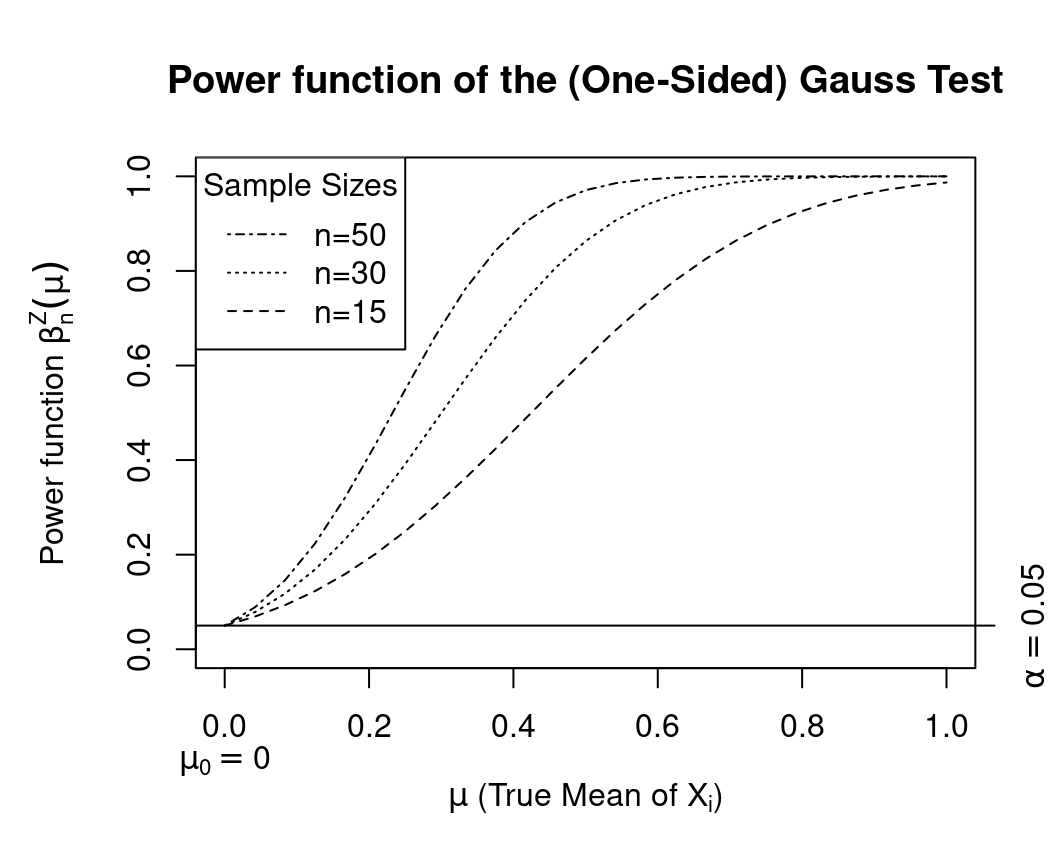
\includegraphics{05-Simulations_files/figure-latex/unnamed-chunk-3-1.pdf}

\hypertarget{simulated-power-function}{%
\subsection{Simulated Power Function}\label{simulated-power-function}}

The power function is best suited to compare several test statistics with each other. Very often, however, it is impossible to compute the power function \(\beta_{n,\alpha}(\theta)\) analytically. (The Gauss test is a rare exception.) The reason for this is that we often know only the distribution of a test statistic under the null hypothesis, but not under the alternative hypothesis. In fact, things can be even worse: Very often, we only know the \textbf{asymptotic distribution} of a test statistic under the null hypothesis. That is, the null distribution is only known for the limiting case of \(n\to\infty\).

\textbf{Solution:}
Use \textbf{Monte-Carlo Simulations} in order approximate the power function.

For the sake of simplicity let's approximate the power function \(\beta^Z_{n,\alpha}(\theta)\) of the one-sided Gauss-Test. This has the (didactic) advantage that we can compare our MC-approximated power function with the theoretical power function.

\textbf{General Idea:}
MC-Simulations make use of the \textbf{Law of Large Numbers}. For instance, by the \href{http://www.statlect.com/asylln1.htm}{Strong Law of Large Numbers} we know that the empirical mean
\[\bar{X}_m\to_{(a.s)}\mu_X\]
converges almost surely (a.s.) to the desired limit \(\mathbb{E}(X)=\mu_X\) as \(m\to\infty\). The only prerequisites are that \(X\) has finite first moments, i.e., \(\mathbb{E}(X)=\mu_X<\infty\), and that \(\bar{X}_m\) is constructed from an i.i.d. sample \(X_1,\dots,X_m\). That is, MC-Simulations use averages in order to approximate mean values.

\textbf{Approximating a Power Function (Theory):}

Remember that
\[
\begin{array}{rcl}
\beta^{Z}_{n,\alpha}(\mu_X)
&=&\mathbb{P}(Z \geq z_{1-\alpha}).
\end{array}
\]

Let us rewrite this probability using the following binary random variable:
\[
V=1_{(Z \geq z_{1-\alpha})},
\]
where \(1_{(\text{TRUE})}=1\) and \(1_{(\text{FALSE})}=0\).
Then we have that
\[
\begin{array}{rcl}
\beta^{Z}_{n,\alpha}(\mu_X)
&=&\mathbb{P}(Z \geq z_{1-\alpha})\,=\,\mathbb{E}(V),
\end{array}
\]
since
\[
\begin{array}{rcl}
\mathbb{E}(V)&=&\underbrace{\mathbb{P}(V=1)}_{\mathbb{P}(Z \geq z_{1-\alpha})\cdot 1}+\underbrace{\mathbb{P}(V=0)\cdot 0}_{=0}.%\,=\,\mathbb{P}(Z \geq z_{1-\alpha}).
\end{array}
\]

Now we have an expression for the power function \(\beta^{Z}_{n,\alpha}(\mu_X)\) in terms of the population mean \(\mathbb{E}(V)\).

By the \textbf{Law of Large Numbers} we know that we can use averages of i.i.d. random variables in order to approximate their population mean. That is,
\[
\frac{1}{m}\sum_{j=1}^m V_j\to_{(a.s)}\mathbb{E}(V)\quad\text{as}\quad m\to\infty,
\]
where \((V_1,\dots,V_m)\) is an iid random sample with \(V_j\sim V=1_{(Z \geq z_{1-\alpha})}\). This approximation can be made \textbf{arbitrarily accurate} as \(m\to\infty\).

\hfill\break

The MC-Simulation proceeds as following:

\begin{enumerate}
\def\labelenumi{\arabic{enumi}.}
\tightlist
\item
  Choose a large number \(m\), for instance, \(m=50,000\).
\item
  Generate realizations
  \[
   (v_1,\dots,v_m)
   \]
  from the MC random sample
  \[
   (V_1,\dots,V_m)=(1_{(Z_1 \geq z_{1-\alpha})},\dots,1_{(Z_m \geq z_{1-\alpha})})
   \]
\item
  Approximate \(\mathbb{E}(V)=\beta^{Z}_{n,\alpha}(\mu_X)\) using the empirical means.
  \[
   \frac{1}{m}\sum_{j=1}^m v_j.
   \]
\end{enumerate}

\hfill\break

\textbf{Approximating a Power Function (Practice):}

Let's start with approximating only the following value of the power function for the one-sided Gauss-Test:
\[
\beta^{Z}_{n=15,\alpha=0.05}(0.5)=0.6147.
\]

First, we set the Monte-Carlo sample size to \(m=50,000\).

Second, we need a realization from the random sample
\[
(1_{(Z_1 \geq z_{1-\alpha})},\dots,1_{(Z_m \geq z_{1-\alpha})}).
\]
In R you can do this as following:

\begin{Shaded}
\begin{Highlighting}[]
\FunctionTok{set.seed}\NormalTok{(}\DecValTok{1009}\NormalTok{)}
\DocumentationTok{\#\# Setup:}
\NormalTok{n         }\OtherTok{\textless{}{-}} \DecValTok{15}    \CommentTok{\# Sample Size}
\NormalTok{alpha     }\OtherTok{\textless{}{-}}  \FloatTok{0.05} \CommentTok{\# Significance Level}
\NormalTok{mu.X.true }\OtherTok{\textless{}{-}}  \FloatTok{0.5}  \CommentTok{\# The (usually unknown) true mean of X\_i}
\NormalTok{mu.X.null }\OtherTok{\textless{}{-}}  \DecValTok{0}    \CommentTok{\# The null{-}hypothesis mean of X\_i}
\NormalTok{var.X     }\OtherTok{\textless{}{-}}  \DecValTok{1}    \CommentTok{\# The (assumed known)  var of X\_i}

\DocumentationTok{\#\# Critical value:}
\NormalTok{z\_crit }\OtherTok{\textless{}{-}} \FunctionTok{qnorm}\NormalTok{(}\DecValTok{1}\SpecialCharTok{{-}}\NormalTok{alpha, }\AttributeTok{mean=}\DecValTok{0}\NormalTok{, }\AttributeTok{sd=}\DecValTok{1}\NormalTok{)}

\DocumentationTok{\#\# Number of Monte{-}Carlo Repetitions:}
\NormalTok{m         }\OtherTok{\textless{}{-}} \DecValTok{50000}

\DocumentationTok{\#\# Container for Z{-}realizations:}
\NormalTok{Z         }\OtherTok{\textless{}{-}} \FunctionTok{rep}\NormalTok{(}\ConstantTok{NA}\NormalTok{, m)}

\DocumentationTok{\#\# MC{-}Experiments:}
\ControlFlowTok{for}\NormalTok{(j }\ControlFlowTok{in} \DecValTok{1}\SpecialCharTok{:}\NormalTok{m)\{}
  \DocumentationTok{\#\# Generate X{-}sample:}
\NormalTok{  X.sample }\OtherTok{\textless{}{-}} \FunctionTok{rnorm}\NormalTok{(}\AttributeTok{n=}\NormalTok{n, }\AttributeTok{mean=}\NormalTok{mu.X.true, }\AttributeTok{sd=}\FunctionTok{sqrt}\NormalTok{(var.X))}
  \DocumentationTok{\#\# Compute jth realization of Z:}
\NormalTok{  Z[j]     }\OtherTok{\textless{}{-}} \FunctionTok{sqrt}\NormalTok{(n)}\SpecialCharTok{*}\NormalTok{(}\FunctionTok{mean}\NormalTok{(X.sample) }\SpecialCharTok{{-}}\NormalTok{ mu.X.null)}\SpecialCharTok{/}\FunctionTok{sqrt}\NormalTok{(var.X)}
\NormalTok{\}}

\DocumentationTok{\#\# Check Z\textgreater{}=z\_crit:}
\FunctionTok{head}\NormalTok{(Z }\SpecialCharTok{\textgreater{}=}\NormalTok{ z\_crit)}
\end{Highlighting}
\end{Shaded}

\begin{verbatim}
## [1]  TRUE  TRUE  TRUE FALSE FALSE  TRUE
\end{verbatim}

\begin{Shaded}
\begin{Highlighting}[]
\FunctionTok{head}\NormalTok{(}\FunctionTok{as.numeric}\NormalTok{(Z }\SpecialCharTok{\textgreater{}=}\NormalTok{ z\_crit))}
\end{Highlighting}
\end{Shaded}

\begin{verbatim}
## [1] 1 1 1 0 0 1
\end{verbatim}

Third, we need to compute the average
\[
\frac{1}{m}\sum_{j=1}^m 1_{(Z_j \geq z_{1-\alpha})}
\]
with respect to the simulated realizations \(1_{(Z_1 \geq z_{1-\alpha})},\dots,1_{(Z_m \geq z_{1-\alpha})}\).

In R you can do this as following:

\begin{Shaded}
\begin{Highlighting}[]
\DocumentationTok{\#\# MC{-}Approximated Power:}
\NormalTok{MC\_power\_n15\_mu0}\FloatTok{.5} \OtherTok{\textless{}{-}} \FunctionTok{mean}\NormalTok{(Z }\SpecialCharTok{\textgreater{}=}\NormalTok{ z\_crit)}
\NormalTok{MC\_power\_n15\_mu0}\FloatTok{.5}
\end{Highlighting}
\end{Shaded}

\begin{verbatim}
## [1] 0.6139
\end{verbatim}

Observe that this approximation is really close to the true value:
~
\(\beta^{Z}_{n=15,\alpha=0.05}(0.5)\,=\,0.6147 =\) \texttt{Gauss.beta(n=15,\ mu.X.true=0.5)}.

\hfill\break

We can write all this as a practical R function \texttt{Gauss.MC.beta()}:

\begin{Shaded}
\begin{Highlighting}[]
\NormalTok{Gauss.MC.beta }\OtherTok{\textless{}{-}} \ControlFlowTok{function}\NormalTok{(}
    \AttributeTok{n         =} \DecValTok{15}\NormalTok{,    }\CommentTok{\# Sample Size}
    \AttributeTok{alpha     =}  \FloatTok{0.05}\NormalTok{, }\CommentTok{\# Significance Level}
    \AttributeTok{mu.X.true =}  \FloatTok{0.5}\NormalTok{,  }\CommentTok{\# The (usually unknown) true mean of X\_i}
    \AttributeTok{mu.X.null =}  \DecValTok{0}\NormalTok{,    }\CommentTok{\# The null{-}hypothesis mean of X\_i}
    \AttributeTok{var.X     =}  \DecValTok{1}\NormalTok{,    }\CommentTok{\# The (assumed known)  var of X\_i}
    \DocumentationTok{\#\#}
    \AttributeTok{m         =} \DecValTok{50000}  \CommentTok{\# Number of Monte{-}Carlo Repetitions:}
\NormalTok{    )\{}

  \DocumentationTok{\#\# Critical value:}
\NormalTok{  z\_crit }\OtherTok{\textless{}{-}} \FunctionTok{qnorm}\NormalTok{(}\DecValTok{1}\SpecialCharTok{{-}}\NormalTok{alpha, }\AttributeTok{mean=}\DecValTok{0}\NormalTok{, }\AttributeTok{sd=}\DecValTok{1}\NormalTok{)}
  \DocumentationTok{\#\# Container for Z{-}realizations:}
\NormalTok{  Z         }\OtherTok{\textless{}{-}} \FunctionTok{rep}\NormalTok{(}\ConstantTok{NA}\NormalTok{, m)}

  \DocumentationTok{\#\# MC{-}Experiments:}
  \ControlFlowTok{for}\NormalTok{(j }\ControlFlowTok{in} \DecValTok{1}\SpecialCharTok{:}\NormalTok{m)\{}
    \DocumentationTok{\#\# Generate X{-}sample:}
\NormalTok{    X.sample }\OtherTok{\textless{}{-}} \FunctionTok{rnorm}\NormalTok{(}\AttributeTok{n=}\NormalTok{n, }\AttributeTok{mean=}\NormalTok{mu.X.true, }\AttributeTok{sd=}\FunctionTok{sqrt}\NormalTok{(var.X))}
    \DocumentationTok{\#\# Compute jth realization of Z:}
\NormalTok{    Z[j]     }\OtherTok{\textless{}{-}} \FunctionTok{sqrt}\NormalTok{(n)}\SpecialCharTok{*}\NormalTok{(}\FunctionTok{mean}\NormalTok{(X.sample) }\SpecialCharTok{{-}}\NormalTok{ mu.X.null)}\SpecialCharTok{/}\FunctionTok{sqrt}\NormalTok{(var.X)}
\NormalTok{  \}}
  \DocumentationTok{\#\# MC{-}Approx Power}
\NormalTok{  MC.power }\OtherTok{\textless{}{-}} \FunctionTok{mean}\NormalTok{(}\FunctionTok{c}\NormalTok{(}\FunctionTok{as.numeric}\NormalTok{(Z }\SpecialCharTok{\textgreater{}=}\NormalTok{ z\_crit)))}
  \DocumentationTok{\#\#}
  \FunctionTok{return}\NormalTok{(MC.power)}
\NormalTok{\}}

\DocumentationTok{\#\# Vectorization:}
\NormalTok{Gauss.MC.beta }\OtherTok{\textless{}{-}} \FunctionTok{Vectorize}\NormalTok{(}\AttributeTok{FUN=}\NormalTok{Gauss.MC.beta, }\AttributeTok{vectorize.args =} \StringTok{"mu.X.true"}\NormalTok{)}
\end{Highlighting}
\end{Shaded}

\textbf{Plot:}

The function \texttt{Gauss.MC.beta()} allows us now to compare the theoretical trajectory of the power function
\(\beta^{Z}_{n,0.05}(\mu_X)\) for \(\mu_X\in\Omega_0\cup\Omega_1\), e.g., for the sample size \(n=30\) with its simulated counterpart.

Here is the R-Code to do this:

\begin{Shaded}
\begin{Highlighting}[]
\DocumentationTok{\#\# Sequence of different mu\_X values (here from 0 to 1):}
\NormalTok{mu.X.true.seq   }\OtherTok{\textless{}{-}} \FunctionTok{seq}\NormalTok{(}\DecValTok{0}\NormalTok{,}\DecValTok{1}\NormalTok{,}\AttributeTok{len=}\DecValTok{25}\NormalTok{)}

\DocumentationTok{\#\# Simulating the trajectory of the power function for n=30:}
\DocumentationTok{\#\# Number of MC{-}Repetitions:}
\NormalTok{m }\OtherTok{\textless{}{-}} \DecValTok{50000}  
\DocumentationTok{\#\# Try also: }
\DocumentationTok{\#\# m \textless{}{-} 100}

\NormalTok{beta.MC.n}\FloatTok{.30}       \OtherTok{\textless{}{-}} \FunctionTok{Gauss.MC.beta}\NormalTok{(}\AttributeTok{n         =} \DecValTok{30}\NormalTok{, }
                                    \AttributeTok{mu.X.true =}\NormalTok{ mu.X.true.seq,}
                                    \AttributeTok{m         =}\NormalTok{ m)}

\DocumentationTok{\#\# Plot}
\FunctionTok{par}\NormalTok{(}\AttributeTok{mar=}\FunctionTok{c}\NormalTok{(}\FloatTok{5.1}\NormalTok{,}\FloatTok{4.1}\SpecialCharTok{+}\DecValTok{1}\NormalTok{,}\FloatTok{4.1}\NormalTok{,}\FloatTok{2.1}\NormalTok{))}
\FunctionTok{plot}\NormalTok{(}\AttributeTok{y=}\DecValTok{0}\NormalTok{, }\AttributeTok{x=}\DecValTok{0}\NormalTok{, }\AttributeTok{type=}\StringTok{"n"}\NormalTok{,}
     \AttributeTok{ylim=}\FunctionTok{c}\NormalTok{(}\DecValTok{0}\NormalTok{,}\DecValTok{1}\NormalTok{),}
     \AttributeTok{xlim=}\FunctionTok{range}\NormalTok{(mu.X.true.seq), }
     \AttributeTok{xlab=}\FunctionTok{expression}\NormalTok{(}\FunctionTok{paste}\NormalTok{(mu,}\StringTok{" (True Mean of "}\NormalTok{, X[i],}\StringTok{")"}\NormalTok{)), }
     \DocumentationTok{\#\# Labels:}
     \AttributeTok{ylab=}\FunctionTok{expression}\NormalTok{(}\FunctionTok{paste}\NormalTok{(}\StringTok{"Power function "}\NormalTok{,beta[n]}\SpecialCharTok{\^{}}\NormalTok{Z,(mu))), }
     \AttributeTok{main=}\StringTok{"Power function of the (One{-}Sided) Gauss Test"}\NormalTok{)}
\DocumentationTok{\#\# Null{-}hypothesis mean:}
\FunctionTok{mtext}\NormalTok{(}\AttributeTok{text =} \FunctionTok{expression}\NormalTok{(mu[}\DecValTok{0}\NormalTok{]}\SpecialCharTok{==}\DecValTok{0}\NormalTok{), }\AttributeTok{side =} \DecValTok{1}\NormalTok{, }\AttributeTok{line =} \DecValTok{2}\NormalTok{, }\AttributeTok{at =} \DecValTok{0}\NormalTok{)}
\DocumentationTok{\#\# Trajectories:}
\FunctionTok{lines}\NormalTok{(}\AttributeTok{y=}\NormalTok{beta.MC.n}\FloatTok{.30}\NormalTok{, }\AttributeTok{x=}\NormalTok{mu.X.true.seq, }\AttributeTok{lty=}\DecValTok{1}\NormalTok{, }\AttributeTok{lwd=}\DecValTok{4}\NormalTok{, }\AttributeTok{col=}\StringTok{"darkorange"}\NormalTok{)}
\FunctionTok{lines}\NormalTok{(}\AttributeTok{y=}\NormalTok{beta.n}\FloatTok{.30}\NormalTok{,    }\AttributeTok{x=}\NormalTok{mu.X.true.seq, }\AttributeTok{lty=}\DecValTok{2}\NormalTok{)}
\DocumentationTok{\#\# Significance Level:}
\FunctionTok{axis}\NormalTok{(}\DecValTok{4}\NormalTok{, }\AttributeTok{at=}\FloatTok{0.05}\NormalTok{, }\AttributeTok{labels =} \FunctionTok{expression}\NormalTok{(alpha}\SpecialCharTok{==}\FloatTok{0.05}\NormalTok{))}
\FunctionTok{abline}\NormalTok{(}\AttributeTok{h=}\FloatTok{0.05}\NormalTok{, }\AttributeTok{lty=}\DecValTok{1}\NormalTok{)}
\DocumentationTok{\#\# Legend:}
\FunctionTok{legend}\NormalTok{(}\StringTok{"topleft"}\NormalTok{, }\AttributeTok{title =} \StringTok{"Power{-}Functions (n=30)"}\NormalTok{, }
       \AttributeTok{legend =} \FunctionTok{c}\NormalTok{(}\StringTok{"MC{-}Approx."}\NormalTok{,}\StringTok{"Theoretical"}\NormalTok{), }
       \AttributeTok{lty=}\FunctionTok{c}\NormalTok{(}\DecValTok{1}\SpecialCharTok{:}\DecValTok{2}\NormalTok{), }\AttributeTok{lwd=}\FunctionTok{c}\NormalTok{(}\DecValTok{4}\NormalTok{,}\DecValTok{1}\NormalTok{), }\AttributeTok{col=}\FunctionTok{c}\NormalTok{(}\StringTok{"darkorange"}\NormalTok{,}\StringTok{"black"}\NormalTok{))}
\end{Highlighting}
\end{Shaded}

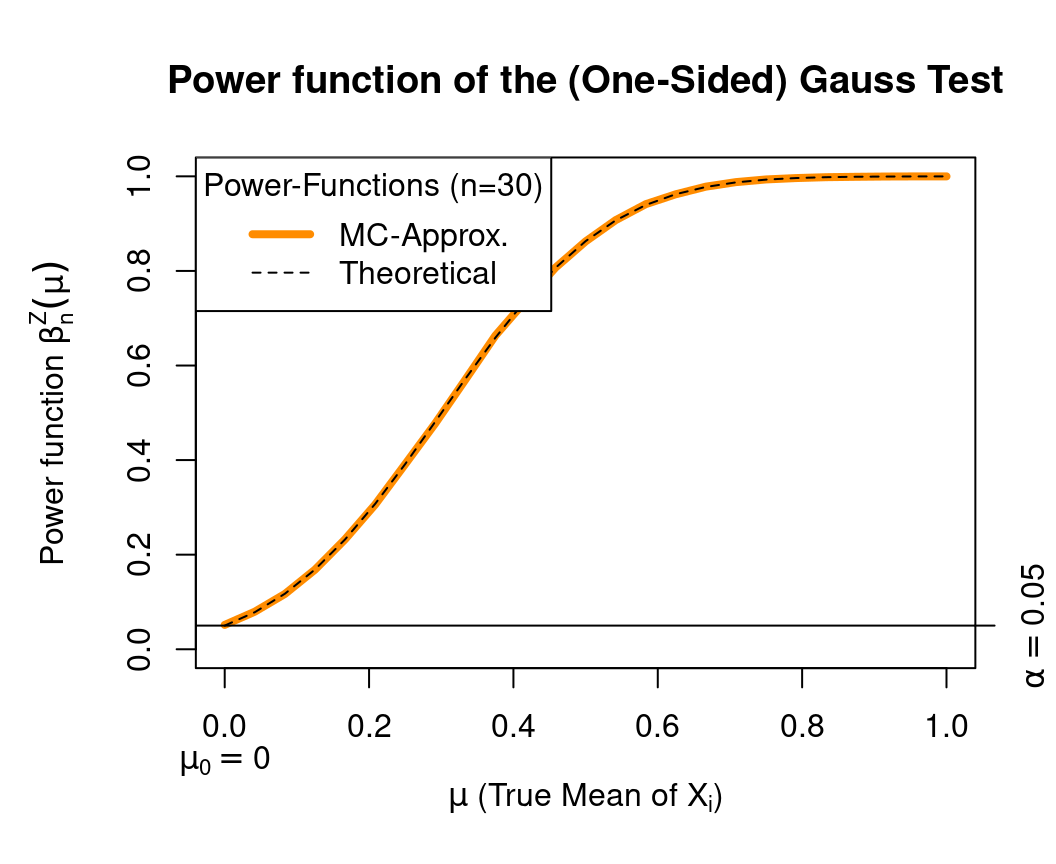
\includegraphics{05-Simulations_files/figure-latex/unnamed-chunk-7-1.pdf}

\hypertarget{checking-parameter-estimators}{%
\section{Checking Parameter Estimators}\label{checking-parameter-estimators}}

For the following, we use our \texttt{myOLSFun()} function to compute OLS estimators.

\begin{Shaded}
\begin{Highlighting}[]
\NormalTok{myOLSFun }\OtherTok{\textless{}{-}} \ControlFlowTok{function}\NormalTok{(y, x, }\AttributeTok{add.intercept=}\ConstantTok{FALSE}\NormalTok{)\{}
  
  \DocumentationTok{\#\# Number of Observations:}
\NormalTok{  n         }\OtherTok{\textless{}{-}} \FunctionTok{length}\NormalTok{(y)}
  
  \DocumentationTok{\#\# Add an intercept to x:}
  \ControlFlowTok{if}\NormalTok{(add.intercept)\{}
\NormalTok{    Intercept }\OtherTok{\textless{}{-}} \FunctionTok{rep}\NormalTok{(}\DecValTok{1}\NormalTok{, n)}
\NormalTok{    x         }\OtherTok{\textless{}{-}} \FunctionTok{cbind}\NormalTok{(Intercept, x)}
\NormalTok{  \}}
  
  \DocumentationTok{\#\# Estimation of the slope{-}parameters:}
\NormalTok{  beta.hat.vec }\OtherTok{\textless{}{-}} \FunctionTok{solve}\NormalTok{(}\FunctionTok{t}\NormalTok{(x) }\SpecialCharTok{\%*\%}\NormalTok{ x) }\SpecialCharTok{\%*\%} \FunctionTok{t}\NormalTok{(x) }\SpecialCharTok{\%*\%}\NormalTok{ y}
  
  \DocumentationTok{\#\# Return the result:}
  \FunctionTok{return}\NormalTok{(beta.hat.vec)}
\NormalTok{\}}
\end{Highlighting}
\end{Shaded}

Let us consider the multiple regression model:

\[y_i=\beta_1 +\beta_2 x_{2i}+\beta_3 x_{3i}+\varepsilon_{i},\quad i=1,\dots,n,\]
where \(\varepsilon_{i}\) is a heteroscedastic error term
\[\varepsilon_{i}\sim N(0,\sigma_i^2),\quad \sigma_i=x_{3i},\]

and where:

\begin{itemize}
\tightlist
\item
  \(i=1,\dots,n\) with \(n=50\)
\item
  \(\beta_1=1\), \(\beta_2=-5\), and \(\beta_3=5\)
\item
  \(x_{2i}\sim N(10,1.5^2)\)
\item
  \(x_{3i}\) comes from a t-distribution with 5 degrees of freedom and non-centrality parameter 2
\end{itemize}

\hfill\break

This following code generates:

\begin{enumerate}
\def\labelenumi{\arabic{enumi}.}
\tightlist
\item
  \texttt{m\ \textless{}-\ 5000} (pseudo) random samples from the above model.
\item
  Computes the OLS estimates \(\hat{\beta}_{2j}\) and \(\hat{\beta}_{3j}\) for each sample \(j=1,\dots,m\)
\item
  Stores the estimation results in the data-vectors \texttt{beta.2.sim} and \texttt{beta.3.sim}
\item
  Plots the distribution of the estimation results using non-parametric density plots
\end{enumerate}

\begin{Shaded}
\begin{Highlighting}[]
\DocumentationTok{\#\# Simulation parameters:}
\FunctionTok{set.seed}\NormalTok{(}\DecValTok{109}\NormalTok{)            }\CommentTok{\# Sets the "seed" of the random number generators}
\NormalTok{m           }\OtherTok{\textless{}{-}} \DecValTok{5000}      \CommentTok{\# Number of simulation runs}
\DocumentationTok{\#\# Model parameters:}
\NormalTok{beta.vec    }\OtherTok{\textless{}{-}} \FunctionTok{c}\NormalTok{(}\DecValTok{1}\NormalTok{,}\SpecialCharTok{{-}}\DecValTok{5}\NormalTok{,}\DecValTok{5}\NormalTok{) }\CommentTok{\# Slope coefficients}
\NormalTok{n           }\OtherTok{\textless{}{-}} \DecValTok{50}        \CommentTok{\# Number of observations}
\DocumentationTok{\#\# Containers to save simulation results:}
\NormalTok{beta.}\FloatTok{2.}\NormalTok{sim  }\OtherTok{\textless{}{-}} \FunctionTok{rep}\NormalTok{(}\ConstantTok{NA}\NormalTok{,m) }
\NormalTok{beta.}\FloatTok{3.}\NormalTok{sim  }\OtherTok{\textless{}{-}} \FunctionTok{rep}\NormalTok{(}\ConstantTok{NA}\NormalTok{,m) }

\DocumentationTok{\#\# Generate the regressors: }
\DocumentationTok{\#\# Outside of the loop (i.e., \textquotesingle{}conditional on X\textquotesingle{})}
\NormalTok{X}\FloatTok{.1} \OtherTok{\textless{}{-}} \FunctionTok{rep}\NormalTok{(}\DecValTok{1}\NormalTok{, n)}
\NormalTok{X}\FloatTok{.2} \OtherTok{\textless{}{-}} \FunctionTok{rnorm}\NormalTok{(n, }\AttributeTok{mean=}\DecValTok{10}\NormalTok{, }\AttributeTok{sd=}\FloatTok{1.5}\NormalTok{)    }\CommentTok{\# Draw realizations form a normal distr.}
\NormalTok{X}\FloatTok{.3} \OtherTok{\textless{}{-}} \FunctionTok{rt}\NormalTok{(n, }\AttributeTok{df=}\DecValTok{5}\NormalTok{, }\AttributeTok{ncp=}\DecValTok{2}\NormalTok{)           }\CommentTok{\# Draw realizations form a t{-}distr.}
\NormalTok{X   }\OtherTok{\textless{}{-}} \FunctionTok{cbind}\NormalTok{(X}\FloatTok{.1}\NormalTok{, X}\FloatTok{.2}\NormalTok{, X}\FloatTok{.3}\NormalTok{)         }\CommentTok{\# Save as a Nx3{-}dimensional matrix.}

\DocumentationTok{\#\# Setup a progressbar}
\CommentTok{\#pb \textless{}{-} txtProgressBar(min = 0, max = m, style = 3)}

\ControlFlowTok{for}\NormalTok{(rpt }\ControlFlowTok{in} \DecValTok{1}\SpecialCharTok{:}\NormalTok{m)\{}
\NormalTok{  eps }\OtherTok{\textless{}{-}}\NormalTok{ (X}\FloatTok{.3}\NormalTok{)}\SpecialCharTok{*}\FunctionTok{rnorm}\NormalTok{(n, }\AttributeTok{mean=}\DecValTok{0}\NormalTok{, }\AttributeTok{sd=}\DecValTok{1}\NormalTok{) }\CommentTok{\# heteroscadastic error term}
\NormalTok{  y   }\OtherTok{\textless{}{-}}\NormalTok{ X }\SpecialCharTok{\%*\%}\NormalTok{ beta.vec }\SpecialCharTok{+}\NormalTok{ eps         }\CommentTok{\# Dependent variable}
  \DocumentationTok{\#\# Estimation}
\NormalTok{  beta.hat }\OtherTok{\textless{}{-}} \FunctionTok{myOLSFun}\NormalTok{(}\AttributeTok{y=}\NormalTok{y,}\AttributeTok{x=}\NormalTok{X)}
  \DocumentationTok{\#\# Save results}
\NormalTok{  beta.}\FloatTok{2.}\NormalTok{sim[rpt] }\OtherTok{\textless{}{-}}\NormalTok{ beta.hat[}\DecValTok{2}\NormalTok{]}
\NormalTok{  beta.}\FloatTok{3.}\NormalTok{sim[rpt] }\OtherTok{\textless{}{-}}\NormalTok{ beta.hat[}\DecValTok{3}\NormalTok{]}
  \DocumentationTok{\#\# Progress bar}
  \CommentTok{\#setTxtProgressBar(pb, rpt)}
\NormalTok{\}}
\CommentTok{\#close(pb)\# Close progressbar}


\CommentTok{\# Theoretical variance covariance matrix of \textbackslash{}hat\{beta\}}
\NormalTok{Var\_beta\_mat }\OtherTok{\textless{}{-}} \FunctionTok{solve}\NormalTok{(}\FunctionTok{t}\NormalTok{(X)}\SpecialCharTok{\%*\%}\NormalTok{X) }\SpecialCharTok{\%*\%} \FunctionTok{t}\NormalTok{(X) }\SpecialCharTok{\%*\%} \FunctionTok{diag}\NormalTok{((X}\FloatTok{.3}\NormalTok{)}\SpecialCharTok{\^{}}\DecValTok{2}\NormalTok{) }\SpecialCharTok{\%*\%}\NormalTok{ X }\SpecialCharTok{\%*\%} \FunctionTok{solve}\NormalTok{(}\FunctionTok{t}\NormalTok{(X)}\SpecialCharTok{\%*\%}\NormalTok{X)}

\DocumentationTok{\#\# Plot results}
\FunctionTok{par}\NormalTok{(}\AttributeTok{mfrow=}\FunctionTok{c}\NormalTok{(}\DecValTok{1}\NormalTok{,}\DecValTok{2}\NormalTok{))}
\FunctionTok{hist}\NormalTok{(beta.}\FloatTok{2.}\NormalTok{sim, }\AttributeTok{prob=}\ConstantTok{TRUE}\NormalTok{, }\AttributeTok{main=}\FunctionTok{expression}\NormalTok{(}\FunctionTok{hat}\NormalTok{(beta)[}\DecValTok{2}\NormalTok{]), }\AttributeTok{ylim=}\FunctionTok{c}\NormalTok{(}\DecValTok{0}\NormalTok{,}\FloatTok{1.55}\NormalTok{))}
\FunctionTok{curve}\NormalTok{(}\FunctionTok{dnorm}\NormalTok{(x, }\AttributeTok{mean=}\NormalTok{beta.vec[}\DecValTok{2}\NormalTok{], }\AttributeTok{sd=}\FunctionTok{sqrt}\NormalTok{(Var\_beta\_mat[}\DecValTok{2}\NormalTok{,}\DecValTok{2}\NormalTok{])), }
      \AttributeTok{col=}\StringTok{"darkblue"}\NormalTok{, }\AttributeTok{lwd=}\DecValTok{2}\NormalTok{, }\AttributeTok{add=}\ConstantTok{TRUE}\NormalTok{, }\AttributeTok{yaxt=}\StringTok{"n"}\NormalTok{)}
\FunctionTok{hist}\NormalTok{(beta.}\FloatTok{3.}\NormalTok{sim, }\AttributeTok{prob=}\ConstantTok{TRUE}\NormalTok{, }\AttributeTok{main=}\FunctionTok{expression}\NormalTok{(}\FunctionTok{hat}\NormalTok{(beta)[}\DecValTok{3}\NormalTok{]), }\AttributeTok{ylim=}\FunctionTok{c}\NormalTok{(}\DecValTok{0}\NormalTok{,.}\DecValTok{75}\NormalTok{))}
\FunctionTok{curve}\NormalTok{(}\FunctionTok{dnorm}\NormalTok{(x, }\AttributeTok{mean=}\NormalTok{beta.vec[}\DecValTok{3}\NormalTok{], }\AttributeTok{sd=}\FunctionTok{sqrt}\NormalTok{(Var\_beta\_mat[}\DecValTok{3}\NormalTok{,}\DecValTok{3}\NormalTok{])), }
      \AttributeTok{col=}\StringTok{"darkblue"}\NormalTok{, }\AttributeTok{lwd=}\DecValTok{2}\NormalTok{, }\AttributeTok{add=}\ConstantTok{TRUE}\NormalTok{, }\AttributeTok{yaxt=}\StringTok{"n"}\NormalTok{)}
\end{Highlighting}
\end{Shaded}

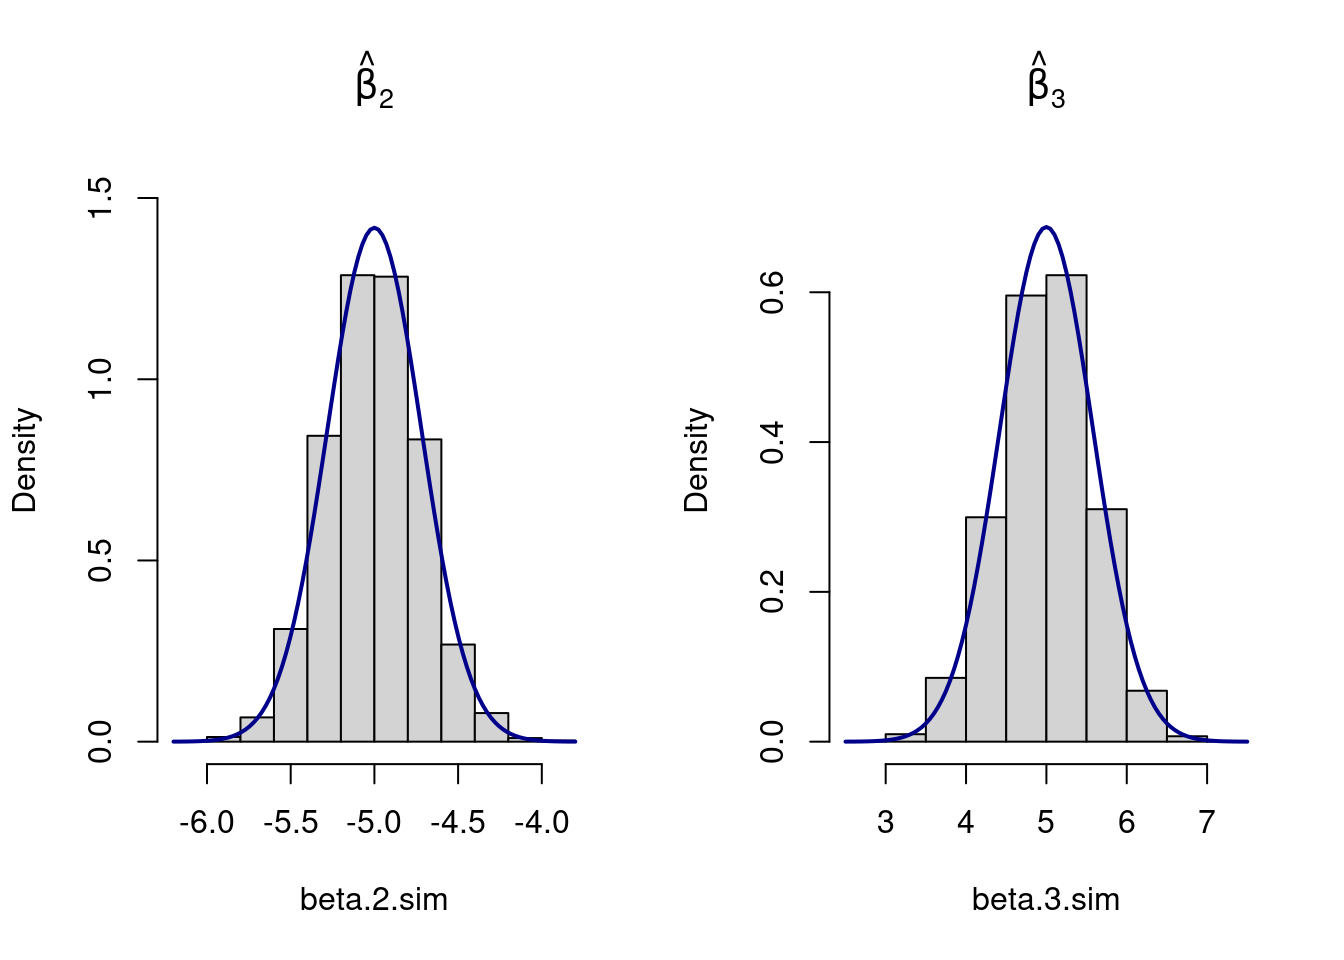
\includegraphics{05-Simulations_files/figure-latex/unnamed-chunk-9-1.pdf}

\hypertarget{how-to-write}{%
\chapter{How to Write}\label{how-to-write}}

\hypertarget{five-common-writing-mistakes}{%
\section{Five Common Writing Mistakes}\label{five-common-writing-mistakes}}

The following is heavily based on a blog-post of \href{https://contemplativemammoth.com/2018/08/21/five-common-writing-mistakes-new-scientists-make/}{Jacquelyn Gill}.

\textbf{1. The passive voice is being used.}
This is an understandable mistake, because not only are we taught to write passively in primary and secondary school science classes, but many of my colleagues still cling to the idea that solid, objective scientific writing must be in the passive voice. However, the passive voice \ldots{}

\begin{itemize}
\tightlist
\item
  results in unnecessarily long sentences and\\
\item
  makes your prose difficult to follow.
\end{itemize}

Why is the active voice better? Because science is an active process, done by human beings: ``I'' and ``we'' statements are appropriate when describing action. For instance, ``We demonstrate the usefulness of our method'' is much nicer to read than ``The usefulness of the method is demonstrated''. The active voice is more engaging to read by its very nature, which makes otherwise dry methods sections just a bit less tedious. We are a storytelling species -- we like a little drama!

\hfill\break

\textbf{2. Extraneous, superfluous or otherwise unnecessary additions.}
\emph{Example of bad writting:} It is entirely likely that your prose is padded with extraneous, superfluous, or otherwise unnecessary additions; furthermore, the utilization of such redundant verbiage is arguably obfuscating your points (thus, in order to improve the clarity of your writing, it is highly recommended that you eschew such stylistic choices, including run-on sentences filled with fluff, padding, and filler).

Perhaps a consequence of assigning papers with word counts, text padding is one of the most common issues with student writing, especially for those writing their first manuscripts. My example sentence above has a few issues:

\begin{enumerate}
\def\labelenumi{\arabic{enumi}.}
\tightlist
\item
  Double (or triple)-dipping with adjectives when one would do
\item
  It crams too much, abusing semi-colons and parentheses for useless purposes
\item
  It's full of ``junk'' phrases that serve no purpose whatsoever.
\end{enumerate}

Tips:

\begin{itemize}
\tightlist
\item
  ``In order to'' is not necessary when ``to'' will do.
\item
  ``It is entirely likely that'' can be replaced with a single word (likely): ``Your prose is likely\ldots{}''
\item
  Words like ``arguably'' or ``furthermore'' or ``thus'' rarely do any heavy lifting in sentences, and are often implied anyway.
\item
  ``Highly'' isn't needed in front of ``likely.''
\item
  ``Utilize'' is rarely more appropriate than ``use.''
\end{itemize}

How to avoid unnecessary additions:

\begin{itemize}
\tightlist
\item
  Relentlessly go over your prose to \textbf{remove junk}.
\item
  When you're over your word count on an abstract or conclusion section, look to cut sentence padding first, before you start cutting your cool ideas.
\item
  Take opportunities to be creative, but not at the expense of clarity.
\end{itemize}

People often assume the thesaurus will help them sound smarter, but instead leaves your reader thinking, ``wow, she/he really loves her/his thesaurus.'' Use fun words sparingly, and \textbf{aim for clarity}.

\hfill\break

\textbf{3. Your prose contains redundant parts.}
You keep making the same point over and over again. I often find myself reading prose that has the same idea presented in multiple ways -- sometimes word for word, from one paragraph to the next! Regardless of how this happens, redundancy highlights the importance of taking a break from your work. Redundancy is also usually a symptom of poor organization; a lack of structure can lead to circular writing, because you don't know where you've come from and you don't have a clear sense of where you're going.

How to avoid redundancies:

\begin{itemize}
\tightlist
\item
  If you're revising your own work, you should be catching the places of redundant text parts.
\item
  Reading your writing out loud helps (you're more likely to catch errors than if you skim the page reading to yourself).
\item
  Get comfortable with deleting your writing. Cutting words/texts is part of the writing process, and sometimes it's the most effective way to make your writing better. That doesn't mean the initial writing was wasted -- it's all part of what got you to cleaner, stronger prose.
\end{itemize}

\hfill\break

\textbf{4. Unclear antecedents.}
When you find yourself writing ``this,'' check to make sure that ``this'' is clearly linked to an antecedent. Remember that your readers aren't in your head, and the connections may not be intuitive. In scientific writing, this problem (haha, see what I did there?) often happens in the beginning of sentences and paragraphs. ``This is a problem, because\ldots{}'' What's the problem?

\hfill\break

\textbf{5. Your paragraph lacks of a topic sentence.}
Each paragraph should have a topic sentence anticipating the main message of the paragraph. Topic sentences help your reader to follow your writing. Furthermore, topic sentences are useful to diagnose structural problems in writing. The sequence of your topic sentences should represent the roadmap of your paper. Therefore, a very quick test to see if you've got organization issues is to check your topic sentences: the first sentence of your paragraph tells your reader what the paragraph is about, and every sentence should serve that topic sentence in some way.

It's worth thinking about the structure before you start writing. Otherwise, you end up taking more of a random walk than a straight line to your point, and it definitely shows. Think about organization early and often -- your topic sentences can help you with it.

As with any rule, you can be a little creative here, but checking your topic sentences are a great way to check for structural issues in your writing.

\hfill\break

\hypertarget{gregory-mankiw-how-to-write-well}{%
\section{Gregory Mankiw: How to Write Well}\label{gregory-mankiw-how-to-write-well}}

The following list of writing guidelines is taken from \href{https://scholar.harvard.edu/mankiw/home}{Gregory Mankiw's} \href{http://gregmankiw.blogspot.com/2006/10/how-to-write-well.html}{Blog}:

\begin{itemize}
\tightlist
\item
  Stay focused. Remember the take-away points you want the reader to remember. If some material is irrelevant to these points, it should probably be cut.
\item
  Keep sentences short. Short words are better than long words. Monosyllabic words are best.
\item
  The passive voice is avoided by good writers.
\item
  Positive statements are more persuasive than normative statements.
\item
  Use adverbs sparingly.
\item
  Avoid jargon. Any word you don't read regularly in a newspaper is suspect.
\item
  Never make up your own acronyms.
\item
  Avoid unnecessary words. For instance, in most cases, change

  \begin{itemize}
  \tightlist
  \item
    ``in order to'' to ``to''
  \item
    ``whether or not'' to ``whether''
  \item
    ``is equal to'' to ``equals''
  \end{itemize}
\item
  Avoid ``of course,''clearly,'' and ``obviously.'' Clearly, if something is obvious, that fact will, of course, be obvious to the reader.
\item
  The word ``very'' is very often very unnecessary.
\item
  Keep your writing self-contained. Frequent references to things that have come before or will come later, can be distracting.
\item
  Put details and digressions in footnotes. Then delete the footnotes.
\item
  Buy a copy of Strunk and White's (Elements of Style){[}\url{https://en.wikipedia.org/wiki/The_Elements_of_Style}{]}. Also, William Zinsser's \emph{On Writing Well}. Read them again and again and again.

  \begin{itemize}
  \tightlist
  \item
    Zinsser's theory is that: ``writing improves in direct ratio to the number of things we can keep out of it.''
  \end{itemize}
\item
  Keep it simple.
\end{itemize}

\hypertarget{rob-j-hyndman-avoid-annoying-a-referee}{%
\section{Rob J Hyndman: Avoid Annoying a Referee}\label{rob-j-hyndman-avoid-annoying-a-referee}}

The following list on ``How to avoid annoying a referee'' is taken from \href{https://robjhyndman.com/hyndsight/how-to-avoid-annoying-a-referee/}{Rob J Hyndman's Blog}:

It's not a good idea to annoy the referees of your paper. They make recommendations to the editor about your work and it is best to keep them happy.

\begin{itemize}
\tightlist
\item
  Explain what you've done clearly, avoiding unnecessary jargon.
\item
  Don't claim your paper contributes more than it actually does.
\item
  Ensure all figures have clear (and well sized) captions and labels.
\item
  Include citations to the referee's own work. Obviously you don't know who is going to referee your paper, but you should aim to cite the main work in the area. It places your work in context, and keeps the referees happy if they are the authors.
\item
  Make sure the cited papers say what you think they say. Sight what you cite!
\item
  Include proper citations for all software packages. If you are unsure how to cite an R package, try the command \texttt{citation("packagename")}.
\item
  Never plagiarize from other papers -- not even sentence fragments. Use your own words. I've refereed a thesis which had slabs taken from my own lecture notes including the typos.
\item
  Don't plagiarize from your own papers. Either reference your earlier work, or provide a summary in new words.
\item
  Provide enough detail so your work can be replicated. Where possible, provide the data and code. Make sure the code works.
\item
  When responding to referee reports, make sure you answer everything asked of you. (See my earlier post \href{https://robjhyndman.com/hyndsight/always-listen-to-reviewers/}{``Always listen to reviewers''})
\item
  If you've revised the paper based on referees' comments, then thank them in the acknowledgements section.
\end{itemize}

\hypertarget{latex}{%
\section{LaTeX}\label{latex}}

Use LaTeX for scientific writing - particularly, if some math is involved! The probably easiest way to start with LaTeX is the online editor of \href{https://overleaf.com/}{overleaf}.

\begin{itemize}
\tightlist
\item
  Overleaf allows you to start writing with LaTeX without installing software.
\item
  Overleaf even allows for collaborative writing.
\end{itemize}

\hfill\break

Alternatively, you can also install a LaTeX-distribtion on your computer. The following brief instructions on how to set up a LaTeX system on different operating systems is taken from \href{https://robjhyndman.com/hyndsight/latex-setup/}{Rob J Hyndman's Blog}:

\textbf{MS-Windows:}

\begin{itemize}
\tightlist
\item
  Download and run the setup program for MikTeX. Choose the ``basic'' system.
\item
  Download and run the installer program for TeXstudio.
\item
  Then run TeXstudio and start typing.
\end{itemize}

\textbf{Mac OS:}

\begin{itemize}
\tightlist
\item
  Download and install MacTeX.
\item
  Then run TeXshop and start typing.
\end{itemize}

\textbf{Ubuntu:}

\begin{itemize}
\tightlist
\item
  Install TexLive and TeXstudio through the software centre.
\item
  Then run Texstudio and start typing.
\end{itemize}

To make sure everything is working ok, open \href{https://robjhyndman.com/research/sample.tex}{sample.tex} in TeXstudio (or TeXshop or TeXworks) to see an example of a LaTeX file. (You will also need \href{https://robjhyndman.com/research/sample.bib}{sample.bib} stored in the same folder.) Click on ``Quick build'' (or hit F1) and the file should be processed and appear in a separate window. Study the difference between the original file and the final product to learn some basic LaTeX commands.

For help with learning LaTeX, check out Rob J Hyndman's \href{https://robjhyndman.com/hyndsight/useful-latex-links/}{``Useful LaTeX links''}.

\hypertarget{how-to-present}{%
\chapter{How to Present}\label{how-to-present}}

The following is heavily based on the paper:

Rob J Hyndman (2011), \href{https://journal.r-project.org/archive/2011-1/RJournal_2011-1_Hyndman.pdf}{Giving a useR! Talk}, The R Journal, 3(1), 69--71

\hfill\break

Giving a talk/presentation is a balancing act in which you have to try to impart some ideas, provide sufficient background and keep the audience interested, all in a very short period of time. I've sat through more than my fair share of bad conference talks. Slides full of equations flashing past quickly, tables containing tiny figures that no-one can read, most of the audience lost on the third slide. Anyone who has attended even one conference will have seen such (bad) presentations.

The problems often stem from confusion about the
purpose of the talk. Some speakers clearly think the
aim of a talk is to impress the audience with their
technical skills, even (or especially) if that means the
audience does not understand what they are talking
about. Others speakers appear to believe that talks
are for those few members of the audience who are
working in the same narrow research area -- and so
no attempt is made to provide an introduction to the
topic. Still others see conference talks as an oral version
of an academic paper, in all its painful detail.

\hypertarget{the-aim-of-your-talk}{%
\section{The Aim of your Talk}\label{the-aim-of-your-talk}}

\begin{itemize}
\tightlist
\item
  I like to think of talks/presentations as \textbf{advertisements for the associated paper}.
\item
  The talk is not intended to cover everything you have done, or even to summarize what you have done.
\item
  In giving a talk, I am hoping that:

  \begin{itemize}
  \tightlist
  \item
    everyone in the audience will have a clear idea of what I have been working on.
  \item
    some of those in the audience will be motivated to read my paper or put into practice some of my advice.
  \end{itemize}
\end{itemize}

The tiny tricky details are for the people who read
the paper. Generally, there is no point discussing the
tiny details of proofs, code or algorithm technicalities. Those
who care will explore the details afterwards.

I tend to spend at least half the time going
through a motivating example and reviewing the
relevant background -- most of the audience will
need that context in order to understand what the
talk is about. In fact, it is reasonable to assume that
the audience knows about as much as you did at the
start of your work in this area. That is, probably very
little. So it is important to spend some time providing
background information or you will lose the audience
quickly. Do not assume the audience already knows what you have spent long hours learning on
your own.

\hypertarget{a-suggested-structure}{%
\section{A Suggested Structure}\label{a-suggested-structure}}

\begin{enumerate}
\def\labelenumi{\arabic{enumi}.}
\tightlist
\item
  Start with a motivating example demonstrating the problem you are trying to solve
\item
  Explain existing approaches to the problem and their weaknesses
\item
  Describe your main contributions
\item
  Show how your ideas solve the problem/example you started with
\end{enumerate}

This structure will not necessarily work for every
talk, but it is a good place to start. In particular, beginning
with a motivating example is much better
than setting up the problem algebraically.

For a 15 minute conference presentation, I divide
the time approximately into 3/4/6/2 minute sections.
Using this structure, you will have barely started
on your own contributions when you are half way
through your allocated time. Resist the temptation to
trim the first two sections. The audience needs time
to absorb the \textbf{purpose of your work} and the context
in which it is set.

\hypertarget{preparing-slides}{%
\section{Preparing Slides}\label{preparing-slides}}

High quality slides are an important part of a good
presentation. I recommend using the beamer package
with LATEX.

\textbf{Avoid distracting slide transitions} and dazzling
slide themes. You want the audience to focus on your
content, not wonder how you implemented some
gimmick. Save animation for aiding interpretation.

Use at least a \textbf{20-point font} so everyone in the
room can read your material.

\textbf{Limit the material on each slide}

\begin{itemize}
\tightlist
\item
  Keep the number of words to a minimum.
\item
  Do not include every detail of what you plan to say.
\item
  Keep it simple.
\item
  Resort to text only when illustrations fail you.
\item
  Very often, a table can be replaced with a suitable
  graphic.
\item
  If you must present tables, only show the essential
  information. No-one is going to read a slide full
  of tiny numbers.
\item
  It is easy, but boring, to have bulleted lists summarizing
  your main points. Instead, use pictures and
  graphics as much as possible.
\item
  Give only the most necessary mathematical details.
  When you use equations, define your notation.
\end{itemize}

\textbf{Slides are not there to remind you what to say}.
Use a page of notes for that purpose. The slides are
for the audience -- make sure everything on your
slides is there because it will help the audience understand
what you are saying.

\textbf{Slide numbers.}It is useful to add slide numbers so the audience
can refer back to specific slides in question time.

\textbf{On your last slide}, give your website or email address
for people to contact you if they want to read
the paper or just ask a
question.

\textbf{Refine the slides.} I spend a lot of time going over my slides looking
for ways to improve them. After a presentation is essentially
complete, I go through all the slides to see
what I can remove -- less text is better. I also look for
places where I can simplify the presentation, where
I can replace text with graphics, and where the titles
can be improved. I often spend almost as much time
refining the slides as in creating the first version.

\textbf{Always preview your slides} on the computer being
used for the talk. You will look foolish if symbols
and Greek letters that looked OK on your computer
translate into something unreadable on the big
screen. Use pdf-slides!

\hypertarget{keeping-to-time}{%
\section{Keeping to Time}\label{keeping-to-time}}

\textbf{Do not deliver a 30-minute talk in 15 minutes.} Nothing
irritates an audience more than a rushed presentation.
It is like trying to get a drink out of a fire hydrant.
Your objective is to engage the audience and
have them understand your message. Do not flood
them with more than they can absorb.

\textbf{Cut your material.} Present only as much material as can reasonably
fit into the allocated time. Generally that means no
more than one slide per minute. I tend to use an average
of about 0.8 slides per minute of talking. It is
helpful to use some slides as time-markers and make
sure you are at the relevant slide at the right time.

\textbf{Never go over time.} Keep an eye out for signals
from the session chair indicating when you need to
conclude. If necessary, be prepared to cut your talk
short and finish with a quick summary.

\textbf{Rehearsing is invaluable.} Practise. Out loud.
Standing up. Using a data projector. Get colleagues
to listen to you, including some who are not knowledgeable
on the topic of your talk; they will be able
to point out places where you may not come across
clearly. After the rehearsal, you may wish to
\textbf{delete some of your material} to ensure the talk can be delivered
within the allocated time.

\textbf{Balance the amount of material} you present with
a reasonable pace of presentation. If you feel rushed
when you practise, then you have too much material.

\hypertarget{giving-the-presentation}{%
\section{Giving the Presentation}\label{giving-the-presentation}}

\textbf{Confidence.} By the time you give the talk, you will have spent
enough time preparing your slides and practising
your talk that you should feel confident of giving a
great presentation.

\textbf{Talking.} Talk at a pace that everybody in the audience can
understand. Speak slowly, clearly, and loudly, especially
if your English is accented. Speak
loudly enough to be easily heard by those sitting in
the back row

\textbf{Engage the audience.} Speak to them, not to the
projector screen or to your notes. It helps to move
around, look at your audience and smile.

\textbf{Do not apologize}

\begin{itemize}
\tightlist
\item
  Never apologize for your slides. Make apologies
  unnecessary by producing great slides in the first
  place. Do not say, ``I know you can't see this, but
  \ldots{}'' If the audience cannot read your slide, there is
  no point displaying it.
\item
  Do not apologize for incomplete results either.
  Researchers understand that all research is incomplete.
  Just present the results and let the audience
  judge. It is okay to say, ``work is on-going''.
\end{itemize}

\textbf{When finished}, thank the audience for their attention.
Stay for the entire session, for the courtesy
and benefit of your audience and your co-speakers.
Afterwards, be available for people to ask you questions.

\hfill\break

\hypertarget{final-advice}{%
\section*{Final Advice}\label{final-advice}}
\addcontentsline{toc}{section}{Final Advice}

My final advise for our last two chapters on writing and presenting:

\begin{quote}
Everything should be made as simple as possible, but not simpler.
\end{quote}

(Quote by Albert Einstein, \href{https://quoteinvestigator.com/2011/05/13/einstein-simple/}{or some other smart person})

  \bibliography{book.bib}

\end{document}
